% Template KLTN cho SV trường ĐHKHTN
% Liên hệ: nqminh@fit.hcmus.edu.vn
% Last update: 08/06/2016

% Chú ý: đọc các phần chú ý đóng khung của file này và chỉnh lại cho phù hợp.
% Trước khi build, xóa hết các file được tạo ra trong quá trình build trước đó, và build theo thứ tự: BIB > PDF > PDF.
% Nếu cập nhật tài liệu tham khảo, cũng cần build lại theo cách trên.

\documentclass[oneside,a4paper,14pt]{extreport}

% Font tiếng Việt
\usepackage[T5]{fontenc}
\usepackage[utf8]{inputenc}
\usepackage[utf8]{inputenc}
\DeclareTextSymbolDefault{\DH}{T1}

% equation
\usepackage{breqn}
\usepackage{amsfonts}
\usepackage{bm}

%table
\usepackage{adjustbox}

\usepackage{pgf}

% Tài liệu tham khảo
\usepackage[
	sorting=nty,
	backend=bibtex,
	defernumbers=true]{biblatex}
\usepackage[unicode]{hyperref} % Bookmark tiếng Việt

\usepackage{pgf}
\addbibresource{References/references.bib}

\makeatletter
\def\blx@maxline{77}
\makeatother

% Chèn hình, các hình trong luận văn được để trong thư mục Images/
\usepackage{graphicx}
\usepackage{caption}
\usepackage{subcaption}
\graphicspath{ {Images/} }

% Chèn và định dạng mã nguồn
\usepackage{listings}
\usepackage{color}
\definecolor{codegreen}{rgb}{0,0.6,0}
\definecolor{codegray}{rgb}{0.5,0.5,0.5}
\definecolor{codepurple}{rgb}{0.58,0,0.82}
\definecolor{backcolour}{rgb}{0.95,0.95,0.92}
\lstdefinestyle{mystyle}{
    backgroundcolor=\color{backcolour},   
    commentstyle=\color{codegreen},
    keywordstyle=\color{magenta},
    numberstyle=\tiny\color{codegray},
    stringstyle=\color{codepurple},
    basicstyle=\footnotesize,
    breakatwhitespace=false,         
    breaklines=true,                 
    captionpos=b,                    
    keepspaces=true,                 
    numbers=left,                    
    numbersep=5pt,                  
    showspaces=false,                
    showstringspaces=false,
    showtabs=false,                  
    tabsize=2
}
\lstset{style=mystyle}

% Chèn và định dạng mã giả
\usepackage{amsmath}
\usepackage{algorithm}
% \usepackage[noend]{algpseudocode}
\usepackage{algpseudocode}
\makeatletter
\def\BState{\State\hskip-\ALG@thistlm}
\makeatother

\DeclareMathOperator*{\argmin}{argmin}

% chèn inline code
\usepackage{xparse}
\NewDocumentCommand{\codeword}{v}{%
    \texttt{\textcolor{blue}{#1}}%
}

% Bảng biểu
\usepackage{multirow}
\usepackage{rotating}
\usepackage{vcell}
\usepackage{array}
\usepackage{diagbox}
\usepackage{booktabs}
\usepackage{colortbl}
\newcolumntype{L}[1]{>{\raggedright\let\newline\\\arraybackslash\hspace{0pt}}m{#1}}
\newcolumntype{C}[1]{>{\centering\let\newline\\\arraybackslash\hspace{0pt}}m{#1}}
\newcolumntype{R}[1]{>{\raggedleft\let\newline\\\arraybackslash\hspace{0pt}}m{#1}}

% Đổi tên mặc định
\renewcommand{\chaptername}{Chương}
\renewcommand{\figurename}{Hình}
\renewcommand{\tablename}{Bảng}
\renewcommand{\contentsname}{Mục lục}
\renewcommand{\listfigurename}{Danh sách hình}
\renewcommand{\listtablename}{Danh sách bảng}
\renewcommand{\appendixname}{Phụ lục}

% Định dạng chapter
\usepackage{titlesec}
\titleformat{\chapter}
    [display] 
    {\normalfont\bfseries\Large}{\chaptername \ \thechapter}{10pt}{\huge}
\titlespacing*{\chapter}{0pt}{-10pt}{40pt} %khoảng cách giữa chapter và đầu trang

\titleformat{\section}
    {\normalfont\bfseries\large}{\thesection}{1em}{}

\titleformat{\subsection}
    {\normalfont\bfseries\normalsize}{\thesubsection}{1em}{}

% Dãn dòng 1.5
\usepackage{setspace}
\onehalfspacing

% Thụt vào đầu dòng
\usepackage{indentfirst}

% Canh lề
\usepackage[
    top=20mm,
    bottom=10mm,
    left=30mm,
    right=20mm,
    footskip = 15mm,
    includefoot]{geometry}

% Trang bìa
\usepackage{tikz}
\usetikzlibrary{calc}
\newcommand\HRule{\rule{\textwidth}{1pt}}

% ========================================================================================= %
% CHÚ Ý: Thông tin chung về KLTN - sinh viên điền vào đây để tự động update các trang khác  %
% ========================================================================================= %
\newcommand{\tenSV}{Nguyễn~Hoàng~Đức~-~Hà~Văn~Duy} % Dấu ~ là khoảng trắng không được tách (các chữ nối với nhau bằng dấu ~ sẽ nằm cùng 1 dòng
\newcommand{\mssv}{18120018~-~18120339}
\newcommand{\tenKL}{Kết~hợp~Template~Matching~và~Deep~Learning~trong~bài~toán~trích~xuất~thông~tin~đơn~thuốc} % Chú ý dấu ~ trong tên khoá luận
\newcommand{\tenGVHD}{ThS.~Lê~Ngọc~Thành~-~ThS.~Trương~Tấn~Khoa}
\newcommand{\tenBM}{Khoa học máy tính}

\begin{document}
% \frontmatter

\begin{titlepage}

    \begin{center}
    %ĐẠI HỌC QUỐC GIA THÀNH PHỐ HỒ CHÍ MINH\\
    TRƯỜNG ĐẠI HỌC KHOA HỌC TỰ NHIÊN\\
    \textbf{KHOA CÔNG NGHỆ THÔNG TIN}\\[2cm]


    { \Large \bfseries \tenSV\\[2cm] } 

    %Tên đề tài Khoá luận tốt nghiệp/Đồ án tốt nghiệp

    { \Large \bfseries KẾT HỢP SO KHỚP MẪU VÀ HỌC SÂU TRONG BÀI TOÁN TRÍCH XUẤT THÔNG TIN ĐƠN THUỐC\\[3cm]} 

% \textit{\Medium (IMPROVED SYSTEM FOR EXTRACTING MEDICINES INFORMATION ON PRINTED PRESCRIPTIONS USING FEATURE PATTERN TECHNIQUES AND DEEP LEARNING METHODS)}
        

    %Chọn trong các dòng sau
    \large KHÓA LUẬN TỐT NGHIỆP CỬ NHÂN\\
    %\large ĐỒ ÁN TỐT NGHIỆP CỬ NHÂN\\
    %\large THỰC TẬP TỐT NGHIỆP CỬ NHÂN\\
    %Đưa vào dòng này nếu thuộc chương trình Chất lượng cao, hoặc lớp Cử nhân tài năng
    \large CHƯƠNG TRÌNH CHÍNH QUY\\
    %\large CHƯƠNG TRÌNH CHẤT LƯỢNG CAO\\
    %\large CHƯƠNG TRÌNH CỬ NHÂN TÀI NĂNG\\[2cm]


    \begin{tikzpicture}[remember picture, overlay]
        \draw[line width = 2pt] ($(current page.north west) + (2cm,-2cm)$) rectangle ($(current page.south east) + (-1.5cm,2cm)$);
    \end{tikzpicture}

    \vfill
    Tp. Hồ Chí Minh, tháng 06/2022

    \end{center}

    \pagebreak

    \begin{center}

    TRƯỜNG ĐẠI HỌC KHOA HỌC TỰ NHIÊN\\
    \textbf{KHOA CÔNG NGHỆ THÔNG TIN}\\[2cm]

    {\large \bfseries Nguyễn Hoàng Đức - 18120018\\} 
    {\large \bfseries Hà Văn Duy - 18120339\\[2cm]}

    %Tên đề tài Khoá luận tốt nghiệp/Đồ án tốt nghiệp
    { \Large \bfseries KẾT HỢP SO KHỚP MẪU VÀ HỌC SÂU TRONG BÀI TOÁN TRÍCH XUẤT THÔNG TIN ĐƠN THUỐC\\[3cm]} 


    %Chọn trong các dòng sau
    \large KHÓA LUẬN TỐT NGHIỆP CỬ NHÂN\\
    %\large ĐỒ ÁN TỐT NGHIỆP CỬ NHÂN\\
    %Đưa vào dòng này nếu thuộc chương trình Chất lượng cao, hoặc lớp Cử nhân tài năng
    \large CHƯƠNG TRÌNH CHÍNH QUY\\[2cm]
    %\large CHƯƠNG TRÌNH CHẤT LƯỢNG CAO\\[2cm]
    %\large CHƯƠNG TRÌNH CỬ NHÂN TÀI NĂNG\\[2cm]

    \textbf{GIẢNG VIÊN HƯỚNG DẪN}\\
    \tenGVHD

    \begin{tikzpicture}[remember picture, overlay]
        \draw[line width = 2pt] ($(current page.north west) + (2cm,-2cm)$) rectangle ($(current page.south east) + (-1.5cm,2cm)$);
    \end{tikzpicture}

    \vfill
    Tp. Hồ Chí Minh, tháng 06/2022

    \end{center}

\end{titlepage}
% Sau trang Title, các bạn chèn nhận xét gủa GVHD và GVPB. Nhận xét sẽ được giáo vụ phát sau buổi bảo vệ để các bạn đóng quyển.

\pagenumbering{roman} % Đánh số i, ii, iii, ...

%\addcontentsline{toc}{chapter}{Lời cam đoan}
%\include{Appendix/reassurances}

\addcontentsline{toc}{chapter}{Lời cảm ơn}
\chapter*{Lời cảm ơn}
\label{thanks}

Trước tiên, chúng tôi xin gửi lời cảm ơn chân thành đến ThS. Lê Ngọc Thành. Thầy đã là người luôn ở bên cạnh dìu dắt và hướng dẫn cho chúng tôi kể từ ngày chúng tôi bắt đầu nhận đề tài này. Thầy cũng là người đã nâng đỡ chúng tôi suốt thời gian qua giúp chúng tôi phá bỏ được những giới hạn của bản thân và chạm tới những cột mốc mới. Một lần nữa, chúng tôi xin gửi lời cảm ơn chân thành đến thầy. Quãng thời gian khi cùng nhau hoàn thành đề tài này sẽ là khoảng thời gian đáng trân quý nhất mà chúng tôi sẽ không bao giờ quên. 

Chúng tôi xin gửi lời cảm ơn đến thầy Trương Tấn Khoa cùng đội ngũ cán bộ giảng dạy của Khoa Công nghệ thông tin, Trường Đại học Khoa học Tự nhiên, những người đã trao cho chúng tôi những tri thức nền tảng rất hữu ích và luôn sẵn sàng hỗ trợ chúng tôi trong quá trình thực hiện khoá luận.

Bên cạnh đó, chúng tôi muốn gửi lời cảm ơn đến bạn Võ Thị Hiếu và bạn Trần Ngọc Lan Khanh vì đã cùng nghiên cứu, cùng hỗ trợ chúng tôi trong quá trình làm và hoàn thiện đề tài này.

Và cuối cùng, cảm ơn bạn Hà Văn Duy và bạn Nguyễn Hoàng Đức - thành viên trong nhóm, vì đã cùng nhau đi đến chặng đường cuối của đề tài khóa luận này, một phần góp sức giúp khoa học đến gần với đời sống xã hội, cải thiện, nâng cấp trải nhiệm của mọi người ngày một hiện đại hơn.


\addcontentsline{toc}{chapter}{Đề cương chi tiết}
\chapter*{Đề cương chi tiết}
\label{proposal}


\section*{Thông tin chung}

\begin{itemize}
    \item Tên đề tài: Kết hợp so khớp mẫu và học sâu trong bài toán trích xuất thông tin đơn thuốc.
    \item Tên đề tài bằng tiếng Anh: Combination of template matching and deep learning in extracting prescription information.
    \item Giảng viên hướng dẫn: \tenGVHD
    \item Nhóm sinh viên thực hiện:
    \begin{itemize}
        \item Nguyễn Hoàng Đức - MSSV: 18120018
        \item Hà Văn Duy - MSSV: 18120339
    \end{itemize}

    \item Thời gian thực hiện: Từ 01/2022 đến 07/2022
    \item Loại đề tài: Ứng dụng
\end{itemize}

\section*{Nội dung thực hiện}

\subsection*{Giới thiệu đề tài}

Đã hơn một năm kể từ khi bùng phát đại dịch  Covid-19 và lan rộng ra toàn cầu, trở thành một cuộc khủng hoảng trong lĩnh vực y tế. Đại dịch đã khiến hơn hơn 400 triệu ca nhiễm, 6 triệu ca tử vong và những con số vẫn đang tiếp tục tăng. Tổ chức Y tế Thế giới (WHO) gọi Covid-19 là chu kỳ "hoảng loạn - lãng quên". Sự bành trướng này yêu cầu chúng ta phải thích nghi và sống chung với đại dịch. Tuy nhiên, tình hình dịch bệnh phức tạp
   sinh ra những suy nghĩ tiêu cực cho con người như cảm giác sợ hãi, lạc lối. Điều đó đã khiến cho nhiều người đưa ra những quyết định thiếu sáng suốt khi sử dụng các loại thuốc điều trị bệnh, từ  đó gây ra những hậu quả đáng tiếc, nhẹ thì tiền mất tật mang, nặng thì ảnh hưởng đến tính mạng. Để tránh những trường hợp không may trong quá trình sử dụng thuốc, đòi hỏi cần phải có một hệ thống hỗ trợ người dùng sử dụng đơn thuốc cũng như quản lý thông tin thuốc một cách chính xác và an toàn hơn.
    
    Có thể thấy, đơn thuốc là thứ vô cùng quan trọng đối với những bệnh nhân. Nó chứa đựng nhiều thông tin có giá trị như thông tin bệnh nhân, tên bác sĩ thăm khám, tình trạng bệnh nhân và thông tin về thuốc đi kèm với liều lượng. Dựa vào các tên thuốc được kê đơn mà nhà thuốc mới có thể bán đúng thuốc trị bệnh. Tuy nhiên, việc ghi nhớ thông tin trong đơn thuốc lại không phải là điều đơn giản. Cụ thể đối với tên thuốc, nó thường là các từ khóa chuyên ngành, khó phát âm và không liên hệ nhiều tới cuộc sống.
    
    Với sự bùng nổ của cuộc cách mạng công nghệ 4.0, dữ liệu mở rộng rất nhanh dẫn đến nhu cầu có nhiều công cụ để quản lý thông tin hiệu quả. Việc ghi nhớ và lưu trữ thông tin trong đơn thuốc một cách thủ công hiện nay đang tạo ra một rào cản lớn cho sự phát triển của ngành y tế. Việc thất lạc hồ hơ là điều không hiếm thấy, dẫn đến khó khăn trong việc truy vết và theo dõi hồ sơ bệnh án của bệnh nhân, ảnh hưởng trực tiếp tới sức khỏe của người bệnh cũng như bệnh viện hay nhà thuốc.
    
    
    Với những lý do được trình bày ở trên, nhóm chúng tôi quyết định  thực hiện đề tài này, giúp đưa ra một ứng dụng hỗ trợ con người quản lý đơn thuốc hiệu quả hơn, gián tiếp hỗ trợ bệnh nhân giải quyết những sai sót không đáng có. Một lợi ích mà đề tài nhóm chúng tôi đem lại nữa đó là giúp con người tiếp cận dễ dàng hơn với công nghệ hiện đại, góp phần giúp Việt Nam bắt kịp với sự phát triển trên thế giới.

\subsection*{Mục tiêu đề tài}

Mục tiêu đề tài khóa luận của chúng tôi là:
    \begin{itemize}
     \item Đọc và tìm hiểu những nghiên cứu có liên quan gần đây về những mô hình phát hiện ký tự quang học có thể áp dụng vào đề tài như: Tesseract \cite{smith2007overview}, CTPN \cite{tian2016detecting}, CRAFT \cite{baek2019character},...  
     \item Tìm hiểu và ứng dụng công trình phù hợp hơn trong việc nhận dạng kí tự quang học trong tiếng Việt, cụ thể là VietOCR \cite{VietOCR} .
     \item Tìm ra đặc trưng của đơn thuốc, từ đó thiết kế nên một giải pháp trích xuất thông tin tương ứng dựa trên kỹ thuật mẫu.
     \item Xây dựng, cải tiến một số mô hình xử lý ngôn ngữ tự nhiên phục vụ cho tác vụ hậu xử lý văn bản cũng như trích xuất thuốc.
     \tiem Xây dựng mô hình giải quyết vấn đề nhập nhằng thông tin trong đơn thuốc.
     \item Xây dựng một ứng dụng hỗ trợ người dùng trong quá trình quản lý thông tin thuốc trong đơn thuốc như liều lượng, giá thành, thành phần.
     \item Cải thiện hiệu suất của mô hình xử lý đơn thuốc hiện tại tốt hơn những mô hình trước đây. 
     \item Xây dựng một tập dữ liệu đơn thuốc Việt Nam, phục vụ cho quá trình huấn luyện và kiểm chứng mô hình, góp phần cải tiến mô hình sau này.
     \item Nâng cao khả năng đọc hiểu, nghiên cứu tài liệu và kỹ năng làm việc nhóm.
    \end{itemize}

\subsection*{Phạm vi đề tài}

Phạm vi đề tài khóa luận của chúng tôi được giới hạn trong việc tìm hiểu, cải tiến các mô hình nhận diện ký tự quang học hiện nay như CRAFT \cite{baek2019character}, VietOCR \cite{VietOCR}, CTPN \cite{tian2016detecting}. Ngoài ra, nhóm cũng tìm hiểu, xây dựng một mô hình phân lớp thông tin trong thuốc dựa trên xử lý ngôn ngữ tự nhiên. Cuối cùng, nhóm sử dụng kết hợp phương pháp tìm kiếm mờ để sửa lỗi cho những thông tin thuốc bị sai, đảm bảo chất lượng của kết quả mô hình.

\subsection*{Cách tiếp cận}

 Cách tiếp cận dự kiến trong quá trình thực hiện đề tài:
    \begin{itemize}
        \item Chuẩn bị dữ liệu: Tiến hành thu thập dữ liệu, bao gồm dữ liệu các đơn thuốc và dữ liệu tên thuốc độc lập từ internet nhằm phục vụ cho việc huấn luyện và kiểm nghiệm mô hình.
        \item Xây dựng mô hình và thực nghiệm: Tìm kiếm những tài liệu, bài báo khoa học trên các nền tảng như GoogleScholar, Arxiv, IEEE có liên quan đến lĩnh vực nhận diện ký tự quang học và xử lý ngôn ngữ tự nhiên, từ đó chọn ra phương pháp kỹ thuật mẫu đặc trưng và phương pháp học sâu để giải quyết bài toán đề ra. Sau cùng kiểm nghiệm mô hình trên tập dữ liệu đơn thuốc thu thập được.
        \item So sánh và đánh giá mô hình: So sánh và đánh giá hiệu suất của mô hình với các mô hình nhận diện đơn thuốc hiện có dựa trên nhiều độ đo và tham số như Precision, Recall, H-mean, WER, CER và thời gian thực thi cho một dữ liệu đầu vào.
        \item Tạo ra ứng dụng để đưa vào thực tế: Tìm hiểu và ứng dụng kiến thức về môn nhập môn công nghệ phần mềm để tạo ra một ứng dụng chụp ảnh đơn thuốc và gửi về server để xử lý, sau đó gửi trả kết quả là thông tin đơn thuốc cho người dùng. Người dùng có thể dễ dàng quản lý thông tin thuốc này ngay trên thiết bị di động thông minh.
    \end{itemize}

\subsection*{Kết quả đề tài}

Kết quả dự kiến đề ra cho đề tài khóa luận này:
    \begin{itemize}
        \item Mỗi cá nhân trong nhóm có thể hiểu được tổng quan về nhận dạng ký tự quang học (các mô hình như Tesseract \cite{smith2007overview}, CRAFT \cite{baek2019character}, CTPN \cite{tian2016detecting},...) và một vài kỹ thuật xử lý ngôn ngữ tự nhiên trong việc trích xuất thông tin trong văn bản (pattern extraction, machine learning), có được kỹ năng hiểu và đưa ra quy trình giải quyết vấn đề khi gặp một bài toán liên quan đến những lĩnh vực này.
        \item Đề xuất được một mô hình nhận diện đơn thuốc dựa trên kết quả nghiên cứu, có hiệu suất tốt hơn, cải thiện lên tới 30\% cho kết quả thực nghiệm đối với độ đo H-mean, và giảm một nửa thời gian thực thi so với những mô hình đã có từ trước, giúp mô hình chúng tôi đề xuất có tính thực tế cao và có thể ứng dụng vào cuộc sống.
        \item Đưa lên Google Play một ứng dụng nhận diện đơn thuốc kết hợp lưu trữ thông tin thuốc và được người dùng đón nhận, đánh giá tốt.
    \end{itemize}

\subsection*{Kế hoạch thực hiện}

Kế hoạch thực hiện đề tài khóa luận được trình bày trong bảng sau:

 \begin{table}
    \centering
    \normalsize  
    \begin{adjustbox}{angle=-90}
    \begin{tabular}{|c|c|c|}
    
        \hline 
        Thời gian & Hà Văn Duy & Nguyễn Hoàng Đức \\\hline
        
        1/2022 & \multicolumn{2}{|c|}{Bắt đầu nhận đề tài khoa học và lập nhóm.} \\\hline
        
        1/2022 - 2/2022 & \multicolumn{2}{|c|}{Tìm hiểu các công trình nghiên cứu liên quan. Báo cáo với giảng viên hàng tuần.} \\\hline
        
        2/2022 - 3/2022 & Đề xuất mô hình Xử lý ngôn ngữ & Đề xuất mô hình Nhận dạng ký tự quang học \\\hline
        3/2022 - 4/2022 & \multicolumn{2}{|c|}{Cài đặt mô hình và thử nghiệm trên các bộ dữ liệu đã thu thập.} \\\hline
        
        4/2022 - 5/2022 &  \multicolumn{2}{|c|}{Tối ưu mô hình và viết paper nộp cho một số hội nghị quốc tế.} \\\hline
        5/2022 - 6/2022 & \multicolumn{2}{|c|}{Lập trình ứng dụng nhận diện đơn thuốc và đưa lên Google Play.} \\\hline
        6/2022 - 7/2022 & \multicolumn{2}{|c|}{Viết báo cáo khóa luận và báo cáo kết quả.} \\\hline
    \end{tabular}
    \end{adjustbox}
    \caption{Kế hoạch thực hiện khóa luận}
    
    \end{table}
    
    


% Mục lục, danh sách hình, danh sách bảng
\addcontentsline{toc}{chapter}{Mục lục}
\tableofcontents
\listoffigures
\listoftables

\addcontentsline{toc}{chapter}{Tóm tắt}
\chapter*{Tóm tắt}
\label{abstract}

Nhận dạng tên thuốc từ đơn thuốc đang là bài toán quan trọng, được nhiều người quan tâm trong bối cảnh sức khỏe của con người đang trở thành vấn đề chính mà xã hội có nhu cầu theo dõi, chăm sóc và phát triển, nhất là sau đại dịch. Việc trích xuất và lưu trữ lại tên thuốc trong đơn thuốc mở ra nhiều cơ hội cho không chỉ bản thân người bệnh, mà còn đóng vai trò quan trọng trong sự phát triển và tự động hóa của đời sống xã hội.

Dựa trên nghiên cứu trước đó, khóa luận này tập trung tiến hành nghiên cứu, thử nghiệm và triển khai mô hình mang tên \textit{Nhận dạng đơn thuốc từ đơn thuốc} (\codeword{MEP}) nhằm nhận dạng có hiệu quả tên thuốc từ các đơn thuốc được chụp bởi các thiết bị di động, máy ảnh. Mô hình đề xuất của chúng tôi khai thác thêm một số luật heuristic dựa trên mẫu đặc trưng và mô hình mạng tích chập giãn nở nhằm trích xuất các thông tin cần thiết từ văn bản được trả ra từ kết quả OCR. Mô hình chúng tôi cho ra kết quả rất ấn tượng khi so sánh với phiên bản tiền nghiệm, đạt 0.82 điểm \textbf{H-mean} trên tập dữ liệu đơn thuốc mà chúng tôi thu thập, đề xuất. Ngoài ra, \codeword{MEP} cũng giúp tăng cường hiệu suất nhận dạng và trích xuất tên thuốc, với thời gian xử lý trung bình giảm 2.6 lần, chỉ từ 6.67 giây cho mỗi đơn thuốc.


\clearpage

\pagenumbering{arabic} % Đánh số 1, 2, 3, ...

% \mainmatter
% Các chương nội dung
\chapter{Giới thiệu}
\label{Chapter1}

\section{Đặt vấn đề \& Động lực}

Đã hơn một năm kể từ khi bùng phát đại dịch Covid-19 và lan rộng ra toàn cầu, trở thành
một cuộc khủng hoảng trong lĩnh vực y tế. Đại dịch đã khiến hơn hơn 400 triệu ca nhiễm, 6
triệu ca tử vong và những con số vẫn đang tiếp tục tăng. Tổ chức Y tế Thế giới (WHO) gọi
Covid-19 là chu kỳ "hoảng loạn - lãng quên". Sự bành trướng này yêu cầu chúng ta phải
thích nghi và sống chung với đại dịch. Tuy nhiên, tình hình dịch bệnh phức tạp sinh ra
những suy nghĩ tiêu cực cho con người như cảm giác sợ hãi, lạc lối. Điều đó đã khiến cho
nhiều người đưa ra những quyết định thiếu sáng suốt khi sử dụng các loại thuốc điều trị
bệnh,từ đó gây ra những hậu quả đáng tiếc, nhẹ thì tiền mất tật mang, nặng thì ảnh hưởng
đến tính mạng. Để tránh những trường hợp không may trong quá trình sử dụng thuốc, đòi
hỏi cần phải có một hệ thống hỗ trợ người dùng sử dụng đơn thuốc cũng như quản lý thông
tin thuốc một cách chính xác và an toàn hơn.

Có thể thấy, đơn thuốc là thứ vô cùng quan trọng đối với những bệnh nhân. Nó chứa đựng
nhiều thông tin có giá trị như thông tin bệnh nhân, tên bác sĩ thăm khám, tình trạng bệnh
nhân và thông tin về thuốc đi kèm với liều lượng. Dựa vào các tên thuốc được kê đơn mà
nhà thuốc mới có thể bán đúng thuốc trị bệnh. Tuy nhiên, việc ghi nhớ thông tin trong đơn thuốc lại không phải là điều đơn giản. Cụ thể đối với tên thuốc, nó thường là các từ khóa
chuyên ngành, khó phát âm và không liên hệ nhiều tới cuộc sống.

Với sự bùng nổ của cuộc cách mạng công nghệ 4.0, dữ liệu mở rộng rất nhanh dẫn đến nhu
cầu có nhiều công cụ để quản lý thông tin hiệu quả. Việc ghi nhớ và lưu trữ thông tin trong
đơn thuốc một cách thủ công hiện nay đang tạo ra một rào cản lớn cho sự phát triển của
ngành y tế. Việc thất lạc hồ hơ là điều không hiếm thấy, dẫn đến khó khăn trong việc truy vết
và theo dõi hồ sơ bệnh án của bệnh nhân, ảnh hưởng trực tiếp tới sức khỏe của người
bệnh cũng như bệnh viện hay nhà thuốc.

Với những lý do được trình bày ở trên, nhóm chúng tôi quyết định thực hiện đề tài này, giúp
đưa ra một ứng dụng hỗ trợ con người quản lý đơn thuốc hiệu quả hơn, gián tiếp hỗ trợ
bệnh nhân giải quyết những sai sót không đáng có. Một lợi ích mà đề tài nhóm chúng tôi
đem lại nữa đó là giúp con người tiếp cận dễ dàng hơn với công nghệ hiện đại, góp phần
giúp Việt Nam bắt kịp với sự phát triển trên thế giới.

\section{Phạm vi đề tài}

Trong phạm vi đề tài khóa luận này, chúng tôi tập trung nghiên cứu và tìm hiểu về một số hệ
thống OCR \cite{impedovo1991optical} hiện có mà trong đó gồm 3 giai đoạn chính: Text Detection, Text Recognition và PostOCR. Từ những kiến thức thu thập được, chúng tôi tạo ra một mô hình hoàn chỉnh bao gồm tận dụng những mô hình có sẵn đồng thời thiết kế và xây dựng những phần tối ưu để cho ra một mô hình có khả năng nhận dạng đơn thuốc tên là \codeword{MEP} (Medicines Extraction System on
Prescriptions). Và mục tiêu mà chúng tôi đề ra trong đề tài khóa luận này là:
\begin{itemize}
    \item \textbf{Tác vụ Text Detection}: Tìm hiểu một số mô hình Text Detection hiện có, thử nghiệm
trên tập dữ liệu đề ra và chọn ra mô hình phù hợp nhất để giải quyết cho bài toán
được đề ra.
\item \textbf{Tác vụ Text Recognition}: Tìm hiểu một số mô hình Text Recognition được sử dụng
phổ biến hiện nay. Thách thức đặt ra chính là mô hình đó phải hoạt động tốt đối với
ngôn ngữ là tiếng Việt.
\item \textbf{Tác vụ Post-OCR}: Đề xuất một số phương pháp cũng như mô hình phù hợp để giải
quyết vấn đề xử lý văn bản sau khi OCR để trả về những kết quả phù hợp.
\item Xây dựng một ứng dụng hỗ trợ người dùng trong quá trình quản lý thông tin thuốc
trong đơn thuốc như liều lượng, giá thành, thành phần.
\item Cải thiện hiệu suất của mô hình xử lý đơn thuốc hiện tại tốt hơn những mô hình
trước đây.
\item Xây dựng một tập dữ liệu đơn thuốc Việt Nam, phục vụ cho quá trình huấn luyện và
kiểm chứng mô hình, góp phần cải tiến mô hình sau này.
\item Nâng cao khả năng đọc hiểu, nghiên cứu tài liệu và kỹ năng làm việc nhóm.
\end{itemize}
\section{Đóng góp chính}

Các đóng góp chính của khóa luận của chúng tôi bao gồm hai loại: Đóng góp về mặt lý
thuyết và đóng góp về mặt thực nghiệm.

\subsection{Đóng góp lý thuyết}

\begin{itemize}
    \item Tìm tòi và nghiên cứu một số bài báo nổi tiếng trên thế giới liên quan đến lĩnh vực nhận diện
ký tự quang học, một số thách thức gặp phải và hướng đi của lĩnh vực này trong tương lai.
    \item Khảo sát một số phương pháp cũng như mô hình hoạt động tốt cho các bài toán text
detection và text recognition trên đơn thuốc tiếng Việt. Đề xuất một số mô hình và phương
pháp hậu xử lý văn bản sau khi OCR với mục tiêu hướng đến là giải quyết bài toán đặt ra
của khóa luận.
    \item Mô hình được đề xuất đã chứng minh được sự vượt trội trong quá trình kiểm thử khi đạt
được hiệu suất rất tốt trên bộ dữ liệu đơn thuốc, bên cạnh đó độ chính xác và thời gian cũng
được cải thiện hơn rất nhiều so với mô hình đã có trước đó (sử dụng Tesseract OCR trên
đơn thuốc và sử dụng khoảng cách khoảng cách Levenshtein để tìm kiếm, so khớp văn bản
trên bộ dữ liệu tên thuốc \cite{nguyen2021developing}).
\end{itemize}

\subsection{Đóng góp thực nghiệm}

\begin{itemize}
    \item Thu thập từ nhiều nguồn khác nhau để xây dựng một bộ dữ liệu đơn thuốc Việt Nam có tên là Prescription Datasets, phục
vụ cho quá trình huấn luyện và kiểm chứng mô hình, góp phần cải tiến mô hình sau này.
        \item Cài đặt được một mô hình OCR trên đơn thuốc hoàn chỉnh có tên gọi là \codeword{MEP} (Medicines
Extraction System on Prescriptions). Trong đó, hai mô hình text detection và text reconition
đã được chúng tôi cài đặt lại và sử dụng bộ tham số đã được pretrain sẵn từ những mô hình
đạt được hiệu suất tốt đã có trước đó. Ngoài ra, chúng tôi cũng đã tìm hiểu và cài đặt một phương pháp tìm kiếm trong tác vụ Post-OCR. Và cuối cùng, Các phương pháp và mô hình NLP phục vụ quá trình trích xuất thông tin thuốc được chúng tôi tổng hợp kiến thức từ đó tạo ra. Quá trình huấn luyện mô hình đã
cho ra một bộ tham số phù hợp giúp mô hình đạt được độ chính xác tốt nhất. Kiểm thử và
đánh giá mô hình với bộ dữ liệu mới.
    \item Xây dựng được một ứng dụng quét thông tin tên thuốc trên đơn thuốc có tên là AppDrug.
Chúng tôi dự định sẽ đưa ứng dụng này lên google play trong thời gian tới.
\end{itemize}

\section{Bố cục}

Trong luận văn này, chúng tôi tổ chức nội dung thành 6 chương. Đầu tiên, chương \ref{Chapter1} sẽ giới
thiệu cũng như tóm tắt bài toán và các vấn đề được đặt ra, bên cạnh đó chúng tôi cũng trình
bày về phạm vi, mục tiêu và một số đóng góp. Chương \ref{Chapter2} sẽ giới thiệu về tổng quan lý thuyết
cần nắm và một số nghiên cứu mà chúng tôi đã tìm hiểu được trong quá trình hoàn thiện đề
tài. Chương \ref{Chapter3} đề xuất mô hình và các phương pháp chúng tôi đã sử dụng để giải quyết vấn
đề được đặt ra ở chương \ref{Chapter1}. Trong chương \ref{Chapter4}, chúng tôi trình bày về quá trình thực nghiệm
và bộ dữ liệu được chúng tôi sử dụng. Kết quả của quá trình thực nghiệm sẽ được chúng tôi
sử dụng để phân tích mô hình đề xuất ở chương \ref{Chapter5}. Và cuối cùng, trong chương \ref{Chapter6}, chúng tôi sẽ đưa ra kết luận
và hướng phát triển có thể có trong tương lai.


\chapter{Tổng quan lý thuyết}
\label{Chapter2}

\section{Optical Character Recognition (OCR)}
Đầu tiên, chúng tôi xin được giới thiệu khái quát về định nghĩa về OCR \cite{impedovo1991optical}. OCR hay Optical Character Recognition (dịch là Nhận dạng ký tự quang học) là một công nghệ phát triển
mạnh mẽ, được sử dụng phổ biến thời gian gần đây. Được biết đến như một kỹ thuật scan
dữ liệu chữ viết trên hình ảnh bất kỳ, OCR giúp phát hiện và phân tích vùng văn bản xuất
hiện xung quanh ta, có thể là sách vở, biển báo,… và chuyển nó thành những ký tự số có
thể thao tác được trên máy tính hoặc các thiết bị điện tử.

Từ đó, ta có thể thực hiện những tác vụ như dịch văn bản, tự động bổ sung phần văn bản bị
khiếm khuyết hoặc dùng nó làm đầu vào của những ứng dụng cao cấp hơn (tìm kiếm, xử
lý,…). Từ những lợi ích phía trên mà hệ thống OCR mang lại, ta có thể tiết kiệm được rất
nhiều thời gian, cập nhật được thông tin nhanh và chính xác cũng như những đối tượng
như người khiếm thị có thể được hỗ trợ nhiều hơn (OCR có khả năng quét và đọc các đoạn
văn bản được đưa ra cải thiện khả năng nhận biết xung quanh của họ).

\begin{figure}
\centering
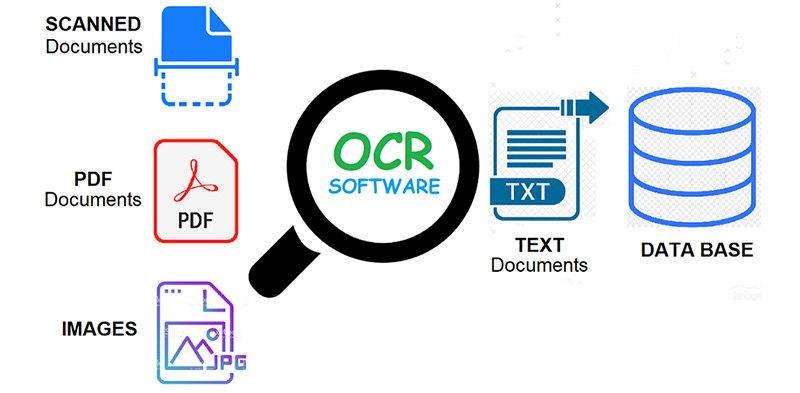
\includegraphics[width=0.9\textwidth]{mep_img/ocr-1.jpg}
\caption{OCR mang lại nhiều lợi ích cho cuộc sống. }\label{fig_2.1}
\end{figure}

\footnotetext{Nguồn tham khảo hình ~\ref{fig_2.1}: https://fpt.ai/vi/tuong-lai-cua-cong-nghe-ocr-song-hanh-cung-ai}

Tuy nhiên bên cạnh những lợi ích to lớn mà OCR mang lại, vẫn còn nhiều hạn chế mà các
mô hình OCR gặp phải:
\begin{itemize}
    \item Độ chính xác của những hệ thống này chưa cao chỉ đạt khoảng 70-80$\%$.
    \item Thời gian hoạt động với hiệu suất của mô hình chưa thật sự tương xứng. Những mô
hình chính xác cao thường có thời gian chạy lâu hơn những mô hình chính xác thấp
rất nhiều.
\item Đa dạng ngôn ngữ thực sự là một rào cản to lớn khi mà ngày càng nhiều đất nước
phát triển. Đi kèm với nó là nhu cầu cần tìm hiểu ngôn ngữ mới của người dùng sẽ ngày một tăng.
\end{itemize}

\begin{figure}
\centering
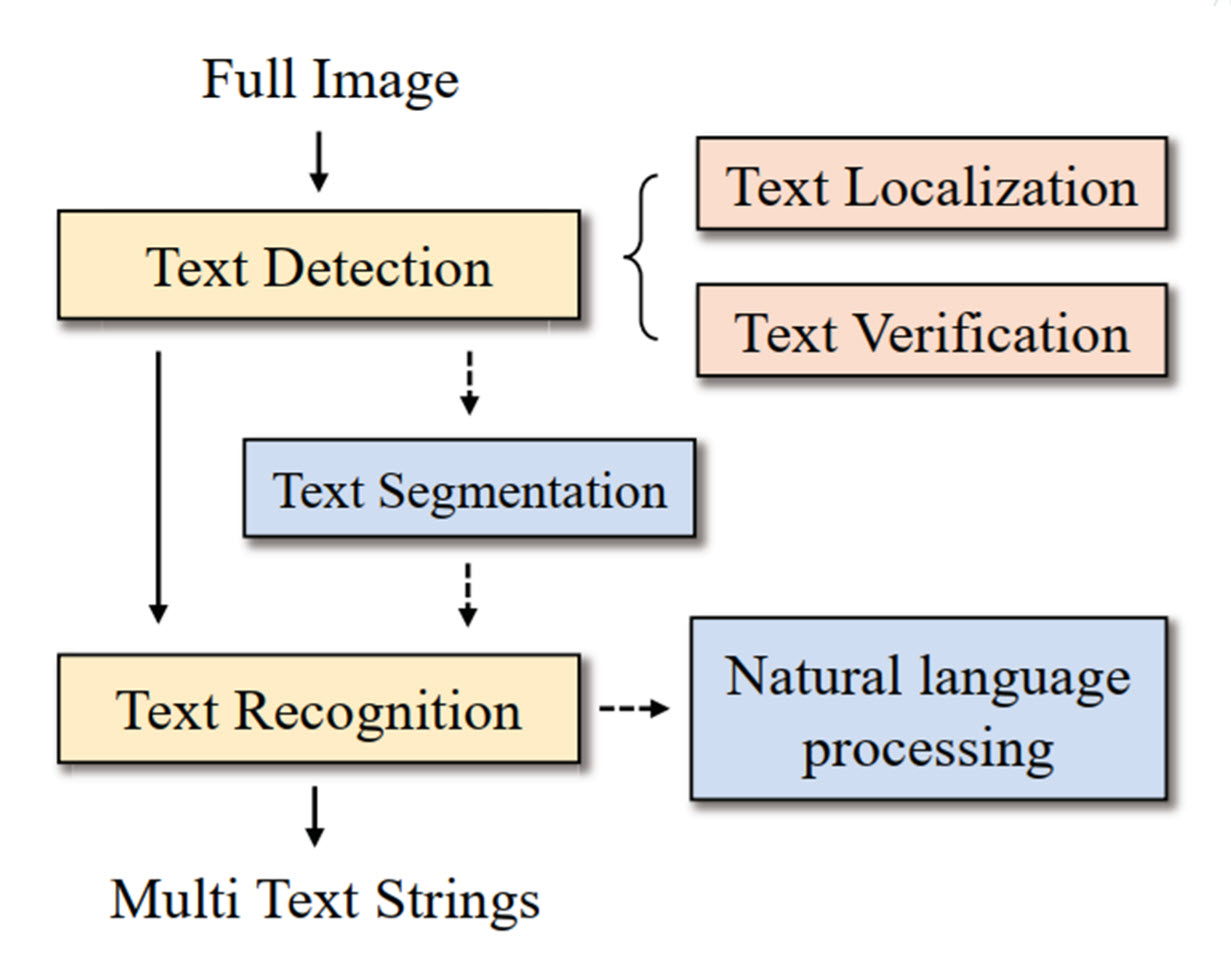
\includegraphics[width=0.9\textwidth]{mep_img/typeofproblem.jpg}
\caption{Mô hình của một số hệ thống OCR phổ biến hiện nay. }\label{fig_2.2}
\end{figure}
\footnotetext{ Nguồn tham khảo hình ~\ref{fig_2.2}: http://tutorials.aiclub.cs.uit.edu.vn/index.php/2021/07/25/ai-tempo-run-gioi-thieu-bai-toan-scene-text/}
Bên cạnh đó còn có rất nhiều lý do khác ảnh hưởng đến kết quả của bài toán OCR như:
font chữ, mật độ văn bản, ảnh nền, cấu trúc, vị trí, độ rõ nét của ảnh,...

Việt Nam là một trong những đất nước có nền kinh tế cũng như du lịch ngày một phát triển.
Nhu cầu về một hệ thống có thể nhận dạng được ngôn ngữ Việt nhưng vẫn đảm bảo về thời
gian và độ chính xác được đặt ra, giữa vô vàn hệ thống OCR có sẵn hiện nay. Trong khóa
luận này chúng tôi cũng sẽ tìm hiểu và cài đặt một mô hình nhận dạng văn bản tiếng Việt - một trong
những công đoạn quan trọng không thể thiếu của mô hình của chúng tôi. Trước tiên, ta cùng
đi tìm hiểu từng thành phần chính của một số mô hình OCR phổ biến hiện nay.



Theo như hình ~\ref{fig_2.2}, một mô hình OCR hiện nay có thể chứa nhiều công đoạn khác nhau như bản địa hóa, khai
thác đặc trưng, phát hiện văn bản và nhận dạng. Nhưng tổng quát, ta sẽ chỉ có ba công
đoạn chính là Text Detection, Text Recognition và Post-OCR.

\subsection{Text Detection}
Nhiệm vụ đầu tiên của một mô hình OCR cơ bản chính là Text Detection. Đây là quá trình
mô hình thực hiện công việc phát hiện vùng văn bản được chứa bởi hình ảnh đầu vào. Đầu
vào của công đoạn này là một hình ảnh bất kỳ và kết quả trả về chính là tọa độ của tập hợp
những bounding box (một ô hình chữ nhật chứa trọn vùng văn bản) của hình ảnh ban đầu.
Có rất nhiều phương pháp có thể được sử dụng để giải quyết bài toán text detection. Có thể
kể đến một số phương pháp truyền thống dựa vào việc xác định các vùng màu sắc, các
vùng chứa biên cạnh có trên ảnh. Các phương pháp này chủ yếu thường dựa vào một số
đặc điểm như màu sắc, hình dạng, kích thước,... của văn bản trên ảnh để có thể tìm kiếm
và trả về vị trí của chúng. Mặc dù những phương pháp kể trên thường có thể dễ dàng áp
dụng lên ảnh với thời gian ngắn trước khi trả về kết quả tuy nhiên độ chính xác của chúng
thì chưa cao.

\begin{figure}
\centering
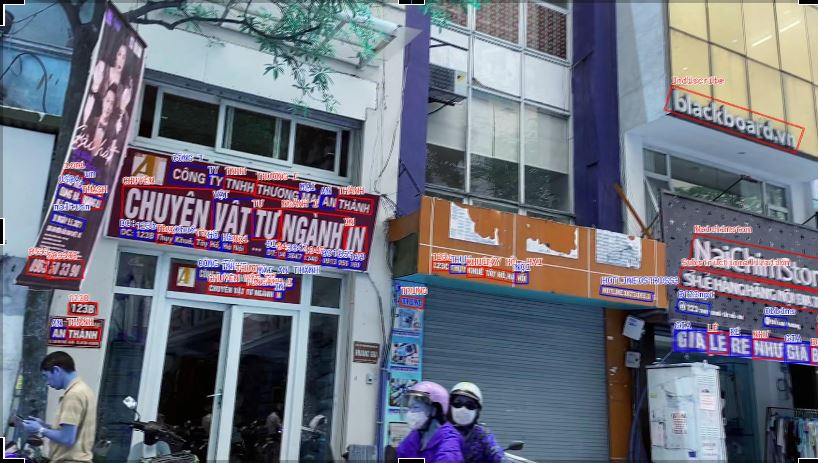
\includegraphics[width=0.9\textwidth]{mep_img/Capture.JPG}
\caption{Số lượng văn bản, nền ảnh và cấu trúc văn bản chính là những khó khăn thường gặp của một mô hình OCR.}\label{fig_2.3}
\end{figure}

Như hình ~\ref{fig_2.3}, nền của ảnh và số lượng văn bản có trong ảnh trở thành một trở ngại vô
cùng lớn trong việc đi tìm những đặc điểm, đặc trưng của văn bản trên ảnh, khiến cho độ
chính xác của những mô hình truyền thống này giảm đi khá đáng kể.
Với sự phát triển của Deep Learning trong những năm gần đây, vô vàn những mô hình Deep
Learning được sinh ra để giải quyết được bài toán text detection trong khoảng thời gian ngắn
nhưng vẫn giữ được độ chính xác cao. Một số hướng giải quyết bài toán text detection
được sử dụng trong thời gian gần đây:
\begin{itemize}
    \item Phát hiện vật thể: Ta có thể coi bài toán phát hiện văn bản là một bài toán phát hiện
vật thể (minh họa hình ~\ref{fig_2.4}), những văn bản có trong ảnh sẽ được định nghĩa và gán nhãn như một vật
thể. Một số mô hình phát hiện vật thể có thể được ứng dụng vào những phương
pháp này như CNNs \cite{delakis2008text}, VGG16 \cite{he2020realtime}, YoLo \cite{haifeng2020natural},... đặc biệt hơn là những mô hình
được sinh ra dựa vào phương pháp này để tập trung hoàn toàn vào nhiệm vụ phát
hiện văn bản như TextFuseNet (ResNeXt-101) \cite{ye2020textfusenet}, EAST \cite{zhou2017east}, CTPN \cite{tian2016detecting},…

\begin{figure}
\centering
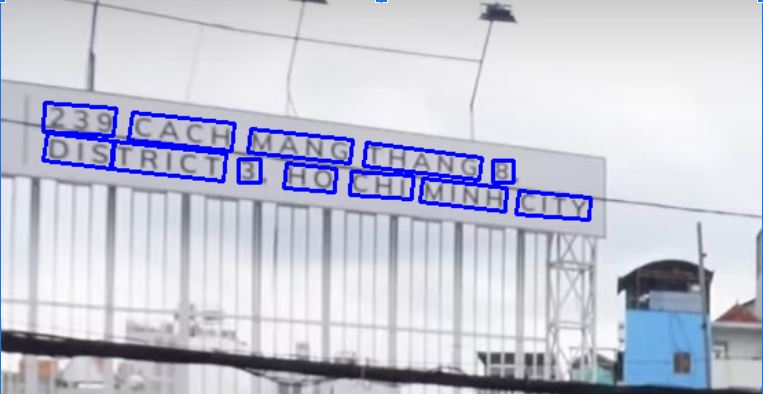
\includegraphics[width=0.9\textwidth]{mep_img/Capture2.JPG}
\caption{Bài toán phát hiện văn bản trở thành bài toán phát hiện vật thể.}\label{fig_2.4}
\end{figure}


\item Phân đoạn vật thể: Bài toán phân đoạn vật thể là một bài toán phân loại từng pixel
trên ảnh thuộc về những lớp nào (minh họa hình ~\ref{fig_2.5}). Để áp dụng phương pháp này vào quá trình phát
hiện văn bản, ta có thể sử dụng một mô hình phân loại pixel để phân loại phần pixel
nào trên ảnh là văn bản. Có thể kể đến U-Nets\cite{fink2018baseline} - một mô hình phân đoạn
ảnh nổi tiếng làm tiền đề cho những mô hình phân đoạn ảnh sau này cho tác vụ
phân đoạn văn bản trên ảnh như CRAFT\cite{baek2019character}.

\begin{figure}
\centering
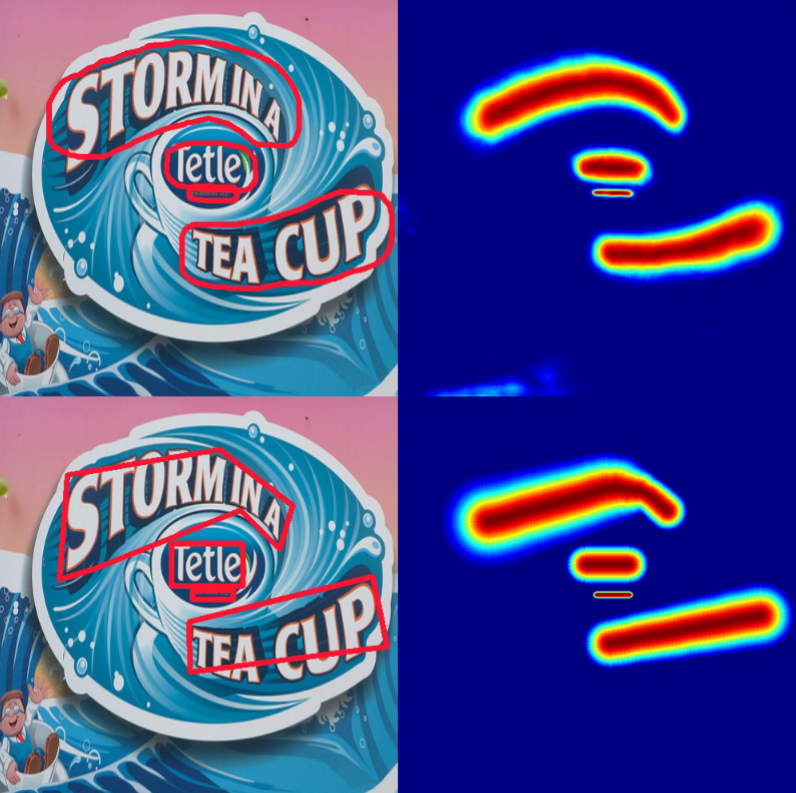
\includegraphics[width=0.9\textwidth]{mep_img/tutorial_segmentation.png}
\caption{Bài toán phát hiện văn bản trở thành bài toán phân đoạn vật thể trên từng pixel.}\label{fig_2.5}
\end{figure}
\footnotetext{ Nguồn tham khảo ~\ref{fig_2.5}: http://tutorials.aiclub.cs.uit.edu.vn/index.php/2021/07/25/ai-tempo-run-gioi-thieu-bai-toan-scene-text/}

\end{itemize}

Baek và các cộng sự đã đề xuất một phương pháp phát hiện văn bản có tên là CRAFT -
Character-Region Awareness For Text detection. Đây là một mô hình khá nổi tiếng và hoạt
động khá tốt trên những tập dữ liệu đa ngôn ngữ. CRAFT thực hiện công việc xác định vùng
của các ký tự đồng thời xác định vùng nối của các ký tự gần nhau. Mặc dù có hiệu suất tốt
nhưng CRAFT lại thực sự kém hiệu quả với những văn bản ở dạng đa hướng vì cấu trúc
của nó khá là khác so với dữ liệu hình ảnh được huấn luyện. Quá trình training mô hình này
được thể hiện như sau:
\begin{itemize}
    \item Đầu tiên, ta phải tạo ra được Synthetic Image, là tập dữ liệu hình ảnh có chưa
những đoạn văn bản được đánh nhãn ở cấp độ ký tự. Ngoài ra, ta sử dụng hai đại
lượng để tính toán độ chính xác của mô hình phát hiện văn bản là region score (có
thể coi đại lượng này giống như IOU - đại lượng đo độ trùng lặp của bounding box
được dự đoán và bounding box nhãn của hình ảnh) và affinity score. Để giải thích về
affinity score, ta có thể giả sử ta có hai ký tự liền kề được đánh nhãn bằng 2
bounding box hình chữ nhật nằm cạnh nhau. Với mỗi hình chữ nhật ta vẽ hai đường chéo, từ hai đường chéo này ta xác định được 2 tam giác trên và dưới. Ta thực hiện
công việc nối tâm của mỗi tam giác lại với nhau tạo thành một tứ giác mới được gọi
là affinity box. Và affinity score được tính toán bởi độ bao phủ hay độ trùng lặp của
các affinity box được mô hình dự đoán ra so với cái affinity box nhãn gốc. Affinity
score được dùng để xác định mỗi quan hệ của 2 từ liền kề nhau xem chúng có phải
cùng thuộc một từ hay không. Quá trình tính toán region score và affinity score được thể hiện ở hình ~\ref{fig_2.6}.

\begin{figure}
\centering
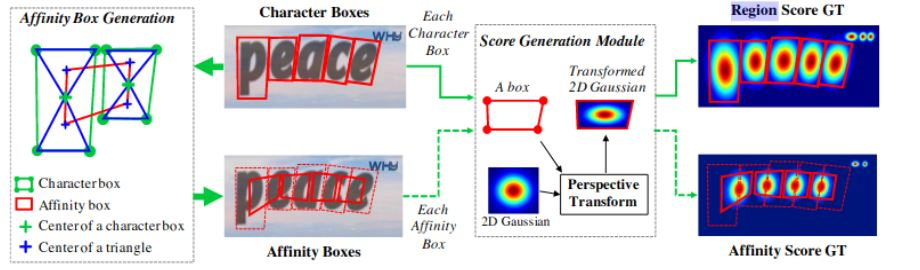
\includegraphics[width=0.9\textwidth]{mep_img/Capture3.JPG}
\caption{Quá trình tính toán của region score và affinity score. }\label{fig_2.6}
\end{figure}
\footnotetext{Nguồn tham khảo hình ~\ref{fig_2.6}: Character Region Awareness for Text Detection \cite{baek2019character}}
\item Ngoài Synthetic Image, ta còn có một bộ dữ liệu ảnh thực được đánh nhãn ở cấp độ
từ được gọi là tập dữ liệu thực tế. CRAFT\cite{baek2019character} sẽ được huấn luyện bằng phương pháp
Weakly-Supervised learning \cite{zhou2018brief}. Trong mỗi lần lặp trong quá trình học (hay còn gọi là
mỗi epoch), mô hình sẽ được đem đi dự đoán trên tập dữ thực tế ở cấp độ từ thành
các bounding box ở cấp độ ký tự. Các đại lượng như Region Score và Affinity Score
đã được giới thiệu ở trên sẽ được tính toán và sử dụng như hàm \textit{loss} để cập nhật lại
trọng số của mô hình bằng Gradient Descent.
\item Kiến trúc chính của CRAFT bao gồm một mạng BackBone dùng để trích xuất những
đặc trưng có trong ảnh như là Resnet18, VGG16 vì chúng đơn giản, không tốn quá
nhiều chi phi và thời gian tính toán. Những đặc trưng này chính là những màu sắc,
cấu trúc, biên cạnh có trong ảnh. Ngoài ra, CRAFT \cite{baek2019character} còn có thêm một số cấu trúc
skip-connection giúp cho mô hình giữ được nhiều thông tin sau khi đi qua nhiều bộ
lọc tích chập và quan trọng nhất là giúp mô hình giảm thiểu tình trạng gradient
vanishing. Bên cạnh đó, vì CRAFT là một trong những phương pháp phân đoạn văn
bản trên ảnh nên mô hình này ít nhiều gì cũng bị ảnh hưởng bởi mô hình mạng
U-Nets. Điển hình ở đây là các lớp De-Convolution hay tích chập ngược và các
skip-connection khiến cho kiến trúc của CRAFT có hình chữ U (giống U-Nets) với các
lớp Convolution đi xuống và De-Convolution đi lên. Kiến trúc của CRAFT \cite{baek2019character} được mô tả kiến trúc ở hình ~\ref{fig_2.7}

\begin{figure}
\centering
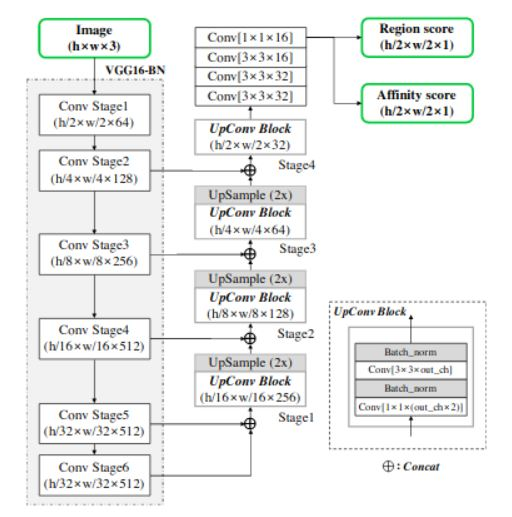
\includegraphics[width=0.9\textwidth]{mep_img/Capture4.JPG}
\caption{Kiến trúc giống mạng U-Nets của mô hình CRAFT. }\label{fig_2.7}
\end{figure}
\footnotetext{Nguồn tham khảo hình ~\ref{fig_2.7}: Character Region Awareness for Text Detection \cite{baek2019character}}
\end{itemize}
Ngoài CRAFT ra, CTPN \cite{tian2016detecting} cũng là một mô hình khá nổi tiếng được sử dụng nhiều trong tác vụ phát hiện văn bản. Mô hình này được phân loại vào nhóm phương pháp phát hiện vật thể (vật thể ở đây chính là văn bản) trên ảnh. Giống như CRAFT, mô hình này cũng sử dụng VGG16 làm một mạng con BackBone trong tác vụ trích xuất đặc trưng trên ảnh. Ngoài ra, Sliding-window - một kỹ thuật trong phát hiện vật thể trên ảnh bằng những bộ lọc tích chập, cũng được sử dụng để tìm vùng nào trên ảnh có thể chứa văn bản. Sau đó, các đặc trưng sẽ được đưa qua một mô hình RNN đơn giản và một lớp fully-connected cuối cùng. Kết quả của mô hình sẽ trả về xác suất có văn bản trong một vùng, tọa độ của bounding box chứa vùng đó. 
\subsection{Text Recognition}
Phần kế tiếp của một mô hình OCR sau khi phát hiện được vị trí của văn bản trong ảnh
chính là nhận diện xem phần văn bản đó là gì, chúng đại diện và thể hiện cho điều gì. Một
số mô hình đạt được hiệu suất tốt trong bài toán này có thể kể đến như Deep Text
Recognition BenchMark \cite{baek2019wrong} và VietOCR \cite{VietOCR}.

Deep Text Recognition BenchMark là một mô hình nhận diện ký tự được đề xuất vào năm 2019. Quá trình hoạt động của mô hình được mô tả
trong hình~\ref{fig_2.8}.

\begin{figure}
\centering
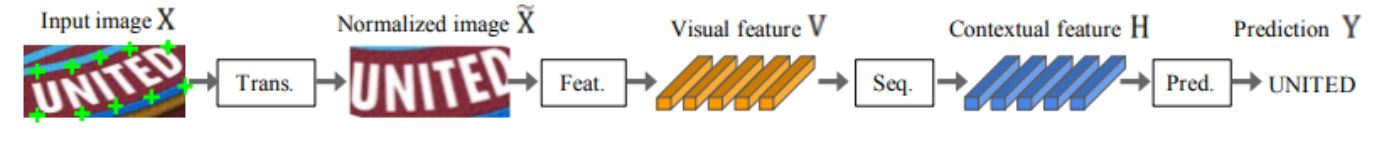
\includegraphics[width=0.9\textwidth]{mep_img/Capture5.JPG}
\caption{Mô hình Deep Text Recognition.}\label{fig_2.8}
\end{figure}
\footnotetext{ Nguồn tham khảo hình ~\ref{fig_2.8}: What Is Wrong With Scene Text Recognition Model Comparisons? Dataset and Model Analysis \cite{baek2019wrong}}
Văn bản có trong hình ảnh (nằm trong 1 bounding box) có thể có nhiều hướng khác nhau
ảnh hưởng đến quá trình dự đoán của mô hình. Nên việc đầu tiên cần làm chính là khử độ
nghiêng, đưa văn bản về 1 hướng duy nhất (các tác giả gọi bước này là chuẩn hóa hình ảnh
ban đầu X thành hình ảnh chuẩn hóa X’). Tiếp theo, hình ảnh đã được chuẩn hóa sẽ được
đưa vào một mô hình mạng BackBone đơn giản để trích xuất đặc trưng như đã nói ở phần
CRAFT, những mạng này có thể là VGG16 hoặc Resnet. Sau đó những đặc trưng được
trích xuất ra sẽ được đưa vào một mô hình đặc biệt được gọi là Sequence Model để huấn
luyện và sẽ giữ lại những đặc trưng liên quan đến ngữ cảnh, từ đó những đặc trưng này sẽ
làm đầu vào cho quá trình nhận diện văn bản.

Mặc dù, mô hình trên được đánh giá là hoạt động tốt trên bộ dữ liệu văn bản tiếng Anh, tuy
nhiên khi sử dụng trên bộ dữ liệu bằng tiếng Việt thì mô hình hoạt động kém hiệu quả. Bởi
lẽ ngôn ngữ Việt có những đặc trưng rất riêng mà tiếng Anh không có. Lấy ví dụ cùng là chữ
A trong tiếng anh, nhưng sang tiếng Việt lại có rất nhiều sắc thái và ngữ nghĩa khác nhau
như: Ă, Á, À,... .

VietOCR \cite{VietOCR} là một mô hình nhận dạng văn bản, chữ viết dành riêng cho người Việt có mã
nguồn mở (miễn phí), có thể dùng với cả chữ viết tay và chữ in. Mô hình này đã kết hợp các
mô hình Deep Learning NLP vào hệ thống Text Recognition làm tăng độ chính xác khi nhận
diện văn bản dựa theo ngữ cảnh. VietOCR cung cấp cho người dùng lựa chọn giữa 2 kiểu
model ngôn ngữ tương ứng với hai kiểu cài đặt Attention OCR và Transformer OCR.

Attention OCR \cite{VietOCR} là sự kết hợp của CNN và Attention Seq2Seq \cite{galassi2020attention}. Đầu vào của mô hình là một
bức ảnh được đưa vào mô hình CNN, sẽ cho một feature maps có kích thước
\textbf{channel*height*width}, và được đưa vào mô hình LSTM để dự đoán. Tuy nhiên, mô hình
LSTM chỉ nhận đầu vào có kích thước là một ma trận đặc trưng 2 chiều. Để giải quyết vấn
đề này, ta thực hiện công việc gộp 2 chiều height và width của ma trận lại làm một, tạo
thành một ma trận mới có kích thước \textbf{channel*(height*width)}. Feature maps lúc này sẽ có
kích thước phù hợp với yêu cầu của mô hình LSTM - đây là một mô hình khá nổi tiếng trong
lĩnh vực Natural Language Processing, mô hình này có khả năng chọn ra những từ nào
trong văn bản là quan trọng, và những đặc trưng của từ đó sẽ trở thành đầu vào cho những
từ tiếp theo trong câu.

Transformer \cite{gillioz2020overview} có thể thay thế cho LSTM để đưa ra dự đoán cho các từ được phát hiện trong
ảnh cũng như các từ có thể xuất hiện tiếp theo. Thay vì xử lý câu một cách tuần tự như
những mô hình ngôn ngữ khác, Transformer thực hiện việc xử lý song song các từ trong
cùng một câu để giảm thời gian xử lý đáng kể. Mô hình này sử dụng cơ chế self-attention,
không giống như kiến trúc hồi quy của RNNs với 6 bộ encoder và 6 bộ decoder. Mỗi
encoder và decoder chứa hai lớp: Self-attention và mạng truyền thẳng (FNN). Self-Attention
giúp cho Transformers có thể hiểu được sự liên quan giữa các từ trong một câu, kể cả khi
chúng có khoảng cách xa. Tuy nhiên một lớp attention được chèn vào giữa các decoder để
mô hình vẫn giữ đươc những đặc trưng và sự liên kết của những từ trước đó.

\subsection{Post-OCR}

Công đoạn cuối cùng của một hệ thống OCR hoàn chỉnh đó chính là Post-OCR, hay hậu xử
lý OCR. Tùy thuộc vào bài toán và từng trường hợp cụ thể gặp phải mà sau khi OCR ta có
những bước xử lý khác nhau. Ví dụ trong bài toán OCR dữ liệu từ sách thành dữ liệu PDF
trên máy. Ta cần một phương pháp hậu xử lý đảm bảo tất cả dữ liệu văn bản được trọn vẹn,
không thiếu sót cũng như không sai chính tả thì thường bên sử dụng hệ thống sẽ chọn
những phương pháp thủ công do con người đích thân chữa lỗi (Survey of post-ocr processing approaches \cite{nguyen2021survey}).

Bên cạnh đó, với sự phát triển của mảng NLP trong thời gian gần đây, việc càng có nhiều
mô hình ứng dụng các mô hình ngôn ngữ vào quá trình hậu xử lý đã không còn quá xa lạ.
Chúng đem lại những kết quả rất tốt, bám sát theo yêu cầu xử lý văn bản mà người dùng
đặt ra. Trong nội dung của khóa luận này, chúng tôi sẽ giới thiệu một số mô hình cũng như
thuật toán có ích trong việc giúp giải quyết bài toán hậu xử lý sau khi OCR đơn thuốc.

\section{Regular Expression}

\textbf{Regular Expression}, hay còn gọi là RegEx, là một công cụ mạnh mẽ để xử lý các loại văn bản. Trong bài toán trích xuất thông tin, đầu vào của ta thường là một tập các thông tin hỗn độn, và ta có nhu cầu chỉ trích ra một phần thông tin có giá trị trong số đó. Nếu như cấu trúc thông tin của input này là tương đối rõ ràng, chúng ta hoàn toàn có thể xây dựng một tập các heuristic rules, hay còn gọi là mẫu (pattern), nhằm lấy được đúng thứ mình cần. Đối với trường hợp này, RegEx là một công cụ mạnh mẽ và tương đối hiệu quả về cả độ chính xác cũng như chi phí thời gian.

Ví dụ, ta có chuỗi "STT: 1 Họ và tên: Nguyễn Văn A", ta có thể dùng luật để tách được số thứ tự, họ tên và giới tính trong chuỗi này theo mẫu như sau: \textbf{"^STT: (.*?) Họ và tên: (.*?) Giới tính: (.*?)$\$$"}. Trong đó, kí tự đầu tiên \textbf{"\^"} đại diện cho đầu dòng văn bản, và\textbf{"\$"} là cuối dòng văn bản. Các cụm ngoặc đơn đại diện cho nội dung mình muốn lấy, bên trong là ".*?" đại diện cho một tập các kí tự bất kì. Hình ~\ref{regex_1} chỉ ra phần giải thích chi tiết cho mẫu này, được chạy thử ở trang \textit{regex101} \footnote{https://regex101.com/r/G9VcLD/1}.

\begin{figure}
\centering
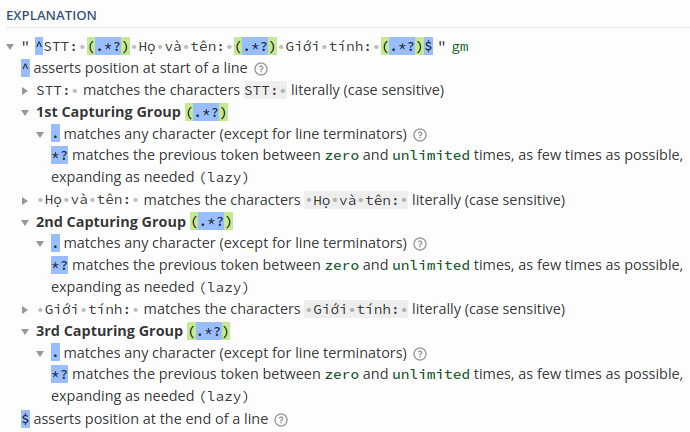
\includegraphics[width=0.8\textwidth]{mep_img/regex_1.png}
\caption{Giải thích chi tiết cho regex trích xuất thông tin người dùng.}\label{regex_1}
\end{figure}

\begin{figure}
\centering
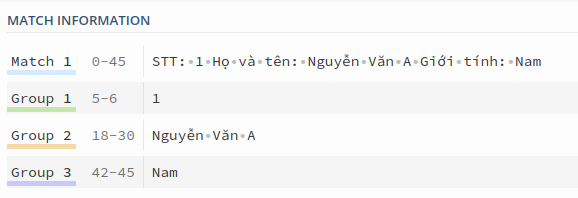
\includegraphics[width=0.8\textwidth]{mep_img/regex_2.png}
\caption{Kết quả thực tế cho RegEx trích xuất thông tin người dùng, bao gồm 3 phần riêng biệt là 3 thông tin mà ta muốn lấy.}\label{regex_2}
\end{figure}

Kết quả của câu RegEx phía trên khi chạy trên dữ liệu ví dụ cho ra được kết quả như trong hình ~\ref{regex_2}. Như vậy, chúng ta hoàn toàn có thể dùng RegEx để ứng dụng vào bài toán trích xuất tên thuốc để đảm bảo tối ưu mô hình. 

\section{TCN}

Để xác định chuỗi văn bản là thuốc nào trong cơ sở dữ liệu, bài toán Text Classification cần được chúng tôi xem xét. Các mô hình dựa trên CNN thường được áp dụng do kết quả thực thi tốt trên các văn bản đơn giản. Tuy nhiên, khi văn bản nhập nhằng hay chứa nhiều đặc trưng khác nhau thì chúng không còn xử lý tốt nữa. Để khắc phục, các mô hình thuộc nhóm \textit{recurrent} (RNN) được đề xuất như LSTM hay GRU. Chúng có thể học được đặc trưng chuỗi liền mạch giống như cách bộ não con người xử lý (theo kiểu trình tự). Từ đó các mô hình này có thể hiểu được thông tin ngữ cảnh dùng trong mỗi văn bản.

Một điểm yếu của các thuật toán dựa trên RNN là chi phí tính toán cao hơn nhiều so với CNN. Shaojie Bai và các cộng sự \cite{bai2018empirical} đã giới thiệu một kỹ thuật mới là temporal convolutional network (TCN). Nó là một phiên bản nhỏ gọn của CNN. Cụ thể, nó dựa trên mạng tích chập giãn nở (dilated convolutions). Các mạng tích chập giãn nở này cho phép TCN học được các đặc trưng trong quá khứ (không bao gồm các thông tin ở tương lai). Mỗi output $y_t$ sẽ dựa trên mỗi chuỗi các input $x$ được lọc (filter size) trên \verb|{0, 1, …, t-1, t}|. Bằng cách chỉnh các tham số \verb|d| (dilation factor) và \verb|k| (filter size), ta có thể quyết định được độ sâu cần thiết trong quá khứ mà mô hình muốn học. 

Với tính giãn nở đó, cách hoạt động của TCN mang lại tính đột phá và có tính \textit{recurrent} tương tự RNN. Điều đó giúp đảm bảo cả về hiệu năng, cũng như cho ra kết quả tốt so với các mô hình thuộc họ RNN. Hình ~\ref{tcn} minh họa kiến trúc của mô hình TCN.

\begin{figure}
\centering
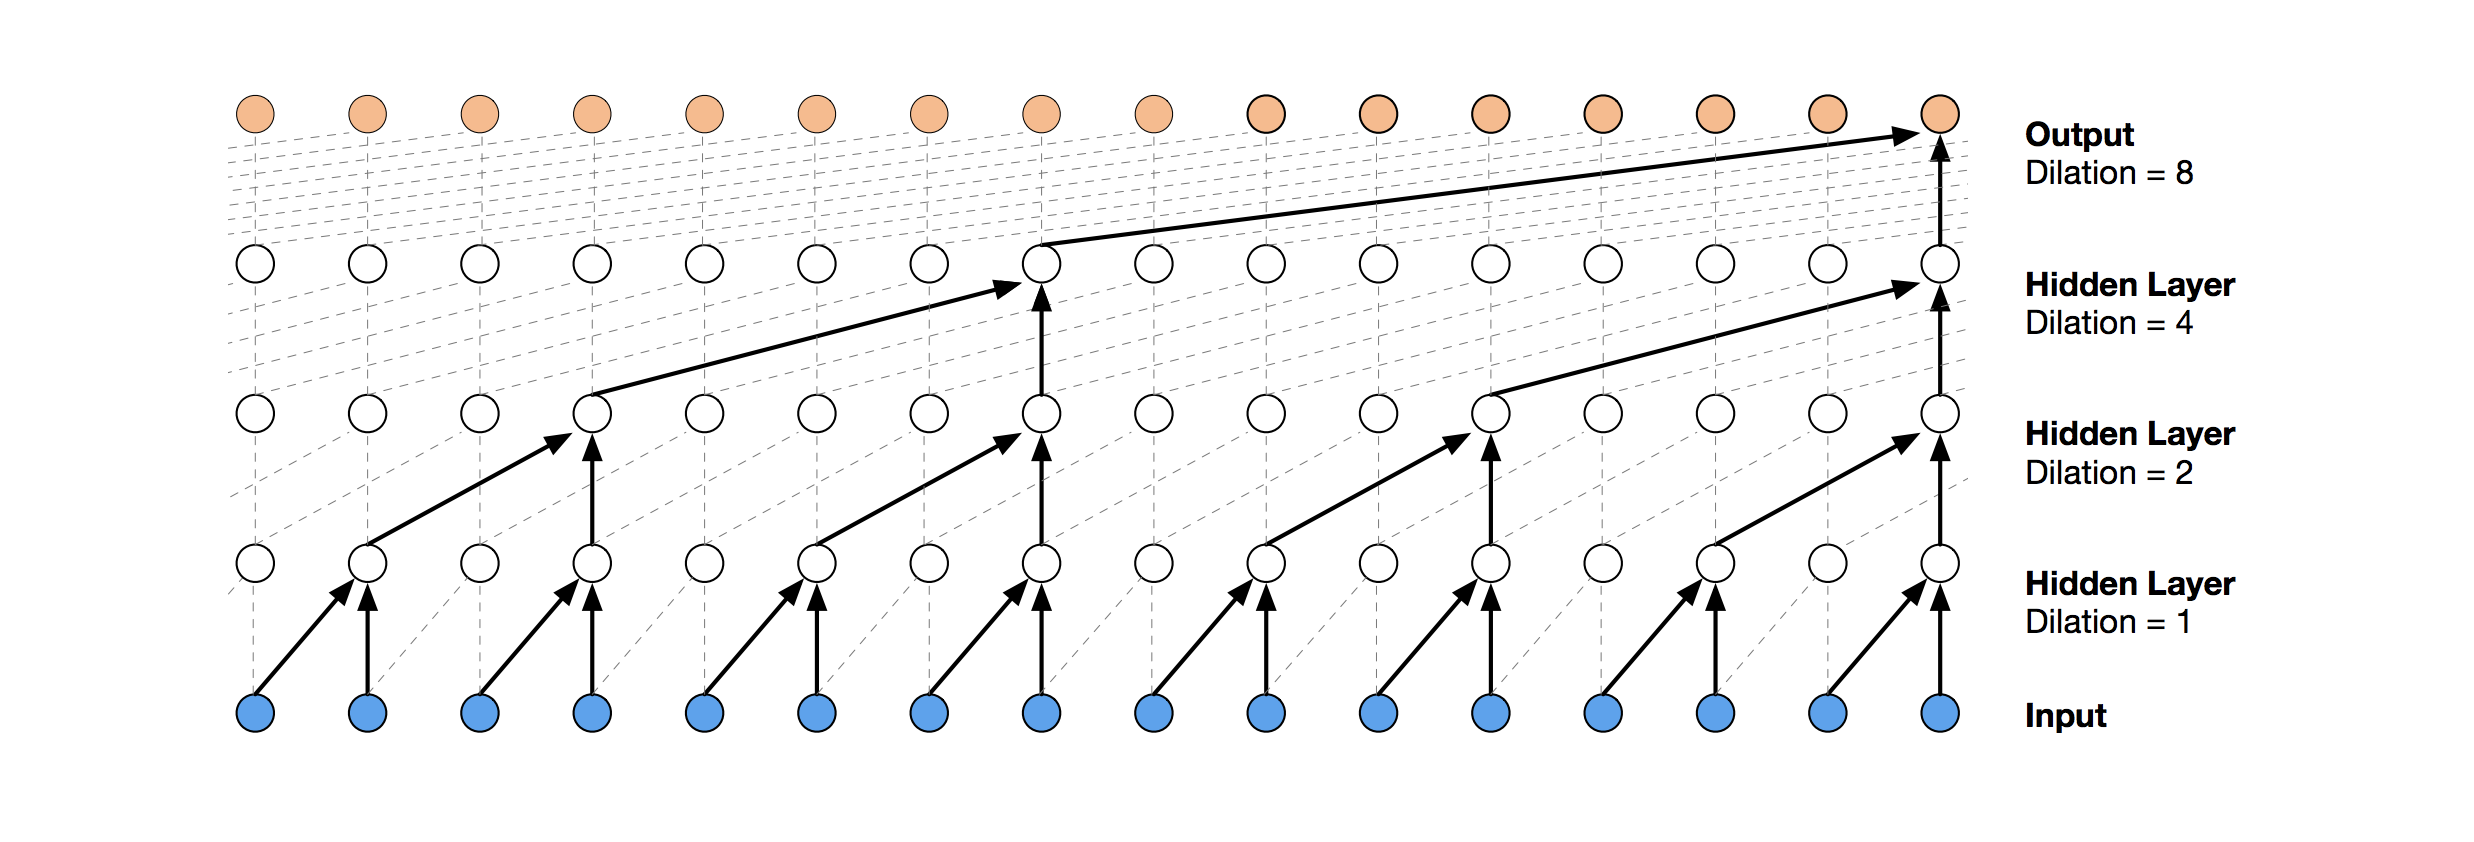
\includegraphics[width=1.0\textwidth]{mep_img/TCN.png}
\caption{Cách hoạt động của kiến trúc mạng TCN, giúp nó có tính liền mạch giống như các mô hình RNN nhưng vẫn đảm bảo xử lý trong thời gian ngắn.}\label{tcn}

\end{figure}

Trong bài toán nhận dạng tên thuốc, ta cũng cần phân biệt tên thuốc, là một hay một số từ có thể mang đặc trưng riêng trong lĩnh vực y học, khác với các văn bản thông thường khác. Như vậy chúng tôi hoàn toàn có thể ứng dụng TCN trong bài toán nhận dạng tên thuốc, và sẽ tiếp tục được đề cập đến ở phần phương pháp đề xuất.

\section{Dataset}

Một trong những yếu tố có thể được coi là quan trọng nhất giúp xây dựng một hệ thống
OCR đạt hiệu suất tốt chính là tập dữ liệu. Trong phần này, chúng tôi sẽ giới thiệu một số
tập dữ liệu được sử dụng trong tác vụ huấn luyện cũng như đánh giá một mô hình OCR.
\begin{itemize}
    \item \textbf{ICDAR 2013}: Đây là bộ dữ liệu có chứa 229 hình ảnh được sử dụng cho quá trình
training mô hình và 233 hình ảnh được dùng cho quá trình đánh giá thời gian và độ
chính xác. Ngoài ra, những phần văn bản có trong ảnh được đánh nhãn ở cấp độ từ
và tập dữ liệu này còn được gọi là tập dữ liệu tiêu chuẩn để đánh giá các mô hình
OCR.
\item \textbf{ICDAR 2015}: Cũng gần giống như tập dữ liệu ICDAR 2013, tập dữ liệu này bao gồm
1000 hình ảnh được dùng cho quá trình training và 500 hình ảnh được dùng cho quá
trình đánh giá. Bộ dữ liệu này được dùng cho rất nhiều cuộc thi về OCR.
\item \textbf{CTW}: Tập dữ liệu bao gồm 32285 hình ảnh với độ phân giải cao và bao gồm hơn 1
triệu ký tự, từ,... . Phần văn bản trong ảnh được đánh nhãn ở cấp độ ký tự.
\end{itemize}
Mặc dù trên thực tế đã có rất nhiều tập dữ liệu khác nhau với kích thước vô cùng lớn và
hình ảnh đa dạng, tuy nhiên với một mô hình phục vụ cho bài toán OCR trên đơn thuốc của
chúng tôi thì những tập dữ liệu trên là chưa đủ. Không giống như những tập dữ liệu kể trên,
với hình ảnh đơn thuốc, vùng chữ thường có khoảng cách rất gần nhau và phông chữ đôi
khi không được đồng đều ảnh hưởng đến quá trình OCR và Post-OCR. Vì thế, chúng tôi đã
thực hiện công việc thu thập và xây dựng một bộ data bám sát vào bài toán và mô hình của
chúng tôi. Bộ dữ liệu đó có tên là \codeword{Prescription Datasets}. Chúng tôi sẽ giới thiệu chi tiết hơn
về tập dữ liệu này trong phần sau.

\chapter{Phương pháp đề xuất}
\label{Chapter3}

Trong chương này, chúng tôi tổng hợp và cài đặt một mô hình giúp trích xuất thông tin tên thuốc từ ảnh, đặt tên là \codeword{MEP}. Đầu vào của mô hình là đơn thuốc, được biểu diễn dưới dạng ảnh. Chúng tôi thực hiện tiền xử lý ảnh sau đó đưa đến CRAFT. CRAFT như đã đề cập tại \cite{baek2019character}, sẽ giúp khoanh vùng các khu vực trên ảnh nơi có thể chứa văn bản. Ưu điểm của CRAFT là nó hỗ trợ khoanh vùng các văn bản theo cấp độ thấp nhất, cấp độ theo từng từ, từ đó sẽ khắc phục được phần lớn các vấn đề liên quan đến ảnh đầu vào ví dụ như bị nghiêng, mờ, lệch,... Các vùng đó sẽ được cắt ra độc lập và đưa đến VietOCR \cite{VietOCR} nhằm mục đích chuyển đổi nó trở thành văn bản. VietOCR là một mô hình mới, hỗ trợ tiếng Anh cũng như rất tốt cho tiếng Việt, giúp hiệu quả của bước nhận dạng đạt tối đa cho các hoá đơn đơn thuốc có chứa nhiều từ tiếng Việt. Bên cạnh đó, chúng tôi cũng xây dựng một thuật toán đặc biệt giúp gom nhóm các từ trên cùng một dòng vào thành một câu, từ đó giúp xây dựng ngữ cảnh của câu một cách rõ ràng trước khi chuyển đến những bước tiếp theo. Tại đây, toàn bộ văn bản được biểu diễn dưới dạng ảnh trong hình ảnh đơn thuốc đã được chuyển đổi thành văn bản mà máy tính và các hệ thống phía sau có thể hiểu được.

Khác với mô hình trước đó, thay vì lấy toàn bộ kết quả của bước OCR ra để so sánh với từ điển thuốc, chúng tôi lựa chọn một con đường khác, trước tiên trích xuất các từ hay cụm từ nằm ở vị trí có thể là tên thuốc trong câu, sau đó kiểm tra chéo với một mô hình tên là Medicine Classifier với nhiệm vụ phân loại tập từ là thuốc ra khỏi tập dữ liệu nhiễu kể trên. Kết quả của bước này là đã ổn định, chỉ cần đưa vào một phần cuối cùng đó là sửa lỗi bằng cách so khớp các tên thuốc đã nhận dạng được với hệ thống từ điển tên thuốc để cho ra kết quả cuối cùng.

Sau đây khoá luận sẽ đi lần lượt qua các phần trong phương pháp đề xuất để làm rõ hơn mục đích và công dụng của các bước trong việc trích xuất thông tin thuốc ra khỏi đơn thuốc. Hình ~\ref{fig_proposed} mô tả lại một cách khái quát các thành phần trong \codeword{MEP}.

\begin{figure}
\centering
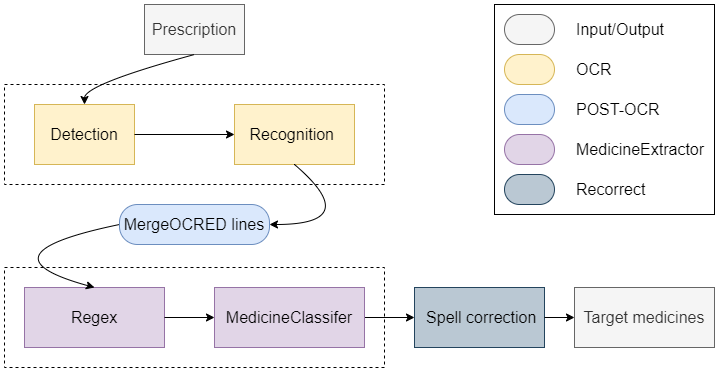
\includegraphics[width=0.9\textwidth]{mep_img/proposed_method.png}
\caption{Cấu trúc của mô hình đề xuất (MEP)}\label{fig_proposed}
\end{figure}

\section{OCR}

Trong phần OCR này, mục tiêu quan trọng cần phải làm là chuyển đổi các ảnh đầu vào thành văn bản mà máy tính có thể hiểu được. Các ảnh đầu vào thường rất đa dạng về cả kiểu dáng, cũng như nội dung. Một ảnh đơn thuốc do người dùng chụp lại đôi khi có thể dựng đứng, đôi khi thì nằm ngang, thậm chí là bị nghiêng dẫn đến cần một thuật toán đủ tốt để trích xuất được văn bản bên trong. Khoá luận sẽ khai thác 2 thành phần trong bước OCR, đó là phát hiện văn bản (Text Detection) và nhận dạng văn bản (Text recognition).

\subsection{Phát hiện văn bản bằng CRAFT}

Chúng tôi lựa chọn CRAFT cho việc phát hiện văn bản dựa trên cách hoạt động của nó. CTPN \cite{tian2016detecting} là một thuật toán phát hiện văn bản tốt, cho phản hồi nhanh tuy nhiên nó không đạt được kết quả ấn tượng đối với đa số ảnh đơn thuốc. Điều đó là do liên quan đến tính chất của phương pháp phát hiện. CRAFT có thể phát hiện từng từ độc lập trong một câu bất kì, trong khi CTPN chú trọng thêm cả vào ngữ cảnh của câu và phát hiện cả dòng tại một thời điểm.

Đối với các hình ảnh đơn thuốc khó phát hiện, ví dụ như bị nghiêng, bị mờ, bị nhiễu hoặc đơn giản là các từ quan trọng trong câu bị che đi, CTPN sẽ bộc lộ rõ nhược điểm rằng trả ra các kết quả nhận dạng không thực sự đúng, không đáp ứng được nhu cầu hiện tại. Ngược lại, dựa trên các bounding box thu thập được từ CRAFT, ta hoàn toàn có thể xây dựng lại cấu trúc câu để đảm bảo ngữ nghĩa cho văn bản được trích xuất nếu cần. Hình ~\ref{fig_craft_pres_2} và ~\ref{fig_craft_pres_1} thể hiện kết quả của CRAFT trên một đơn thuốc cụ thể. 

\begin{figure}
\centering
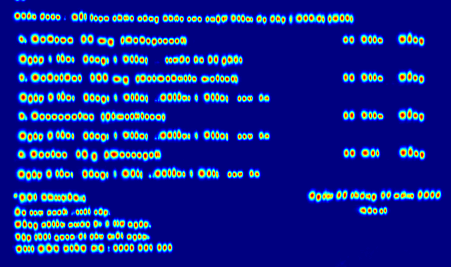
\includegraphics[width=0.9\textwidth]{mep_img/craft_pres_2.png}
\caption{CRAFT phát hiện các thông tin văn bản trong đơn thuốc.}\label{fig_craft_pres_2}
\end{figure}

\begin{figure}
\centering
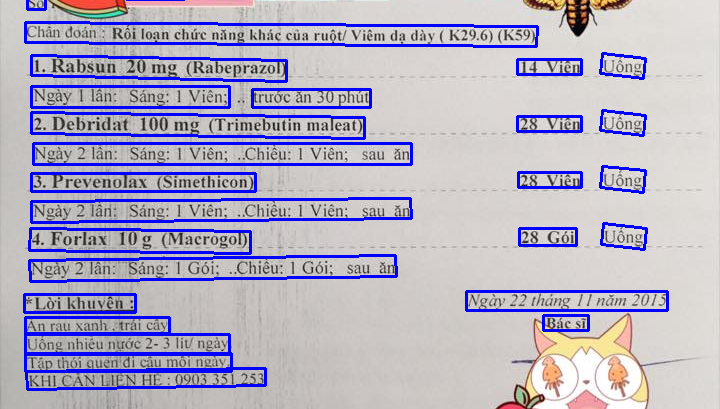
\includegraphics[width=0.9\textwidth]{mep_img/craft_pres_1.png}
\caption{Kết quả phát hiện văn bản của CRAFT trong đơn thuốc sau khi được đóng bounding box.}\label{fig_craft_pres_1}
\end{figure}

\subsection{Nhận dạng văn bản sử dụng VietOCR}

VietOCR \cite{VietOCR} là một mô hình nhận dạng văn bản, chữ viết có hỗ trợ tiếng Việt và đồng thời được người Việt phát triển. Tác giả của VietOCR giới thiệu 2 kiểu cài đặt mô hình, một là Transformers, hai là Sequence-to-sequence (Seq2Seq). Cả 2 hướng cài đặt đều cho ra kết quả tốt, tuy nhiên Transformers hiện đại hơn nhưng lại không có nhiều sự khác biệt về độ chính xác tốt hơn. Vì vậy chúng tôi lựa chọn theo hướng Seq2Seq nhằm tiết kiệm chi phí về mặt thời gian nhận dạng. 

Cách hoạt động của VietOCR đó là nhận dạng theo từng dòng, từ đó chúng tôi có thể sử dụng ngay kết quả trả về của bước phát hiện văn bản bằng CRAFT phía trên làm đầu vào cho VietOCR, mỗi vùng phát hiện văn bản sẽ được nhận dạng và chuyển đổi về văn bản tương ứng. Kết quả của VietOCR sẽ là toàn bộ văn bản trong đơn thuốc.

\section{Medicine Extractor}

Sau khi trải qua bước OCR, chúng ta đã có được toàn bộ văn bản của đơn thuốc. Thông thường, các phương pháp truyền thống sẽ lấy tất cả các văn bản này đưa vào so khớp với một kho dữ liệu gồm từ điển tên thuốc nhằm lọc ra những tên thuốc đúng. Tuy nhiên, kích thước của một bộ từ điển tên thuốc đầy đủ, có chứa đa số tên thuốc hiện đang được lưu hành có kích thước không hề nhỏ. Nếu như ta lấy tất cả văn bản để so sánh thì chi phí so khớp sẽ bị nhân lên gấp nhiều lần. Để khắc phục trường hợp đó, chúng tôi đề xuất một bước bổ sung nhằm cố gắng tối đa lọc ra những cụm từ có khả năng là tên thuốc nhất có thể sao cho vẫn đảm bảo hiệu quả mô hình đồng thời giảm số bước so sánh thêm sau này.

Trong đơn thuốc, ngoài tên thuốc ra thì ta cũng bắt gặp nhiều thông tin khác có thể kể đến như là thông tin bệnh nhân, thông tin cơ sở cấp thuốc, chuẩn đoán bệnh, liều lượng, nguyên liệu, cách sử dụng... Nếu như ta có thể bỏ bớt các thông tin này trước khi so khớp với từ điển thì sẽ cho ra hiệu suất mô hình đạt tốt hơn nhiều so với cách làm cũ.

\begin{figure}
\centering
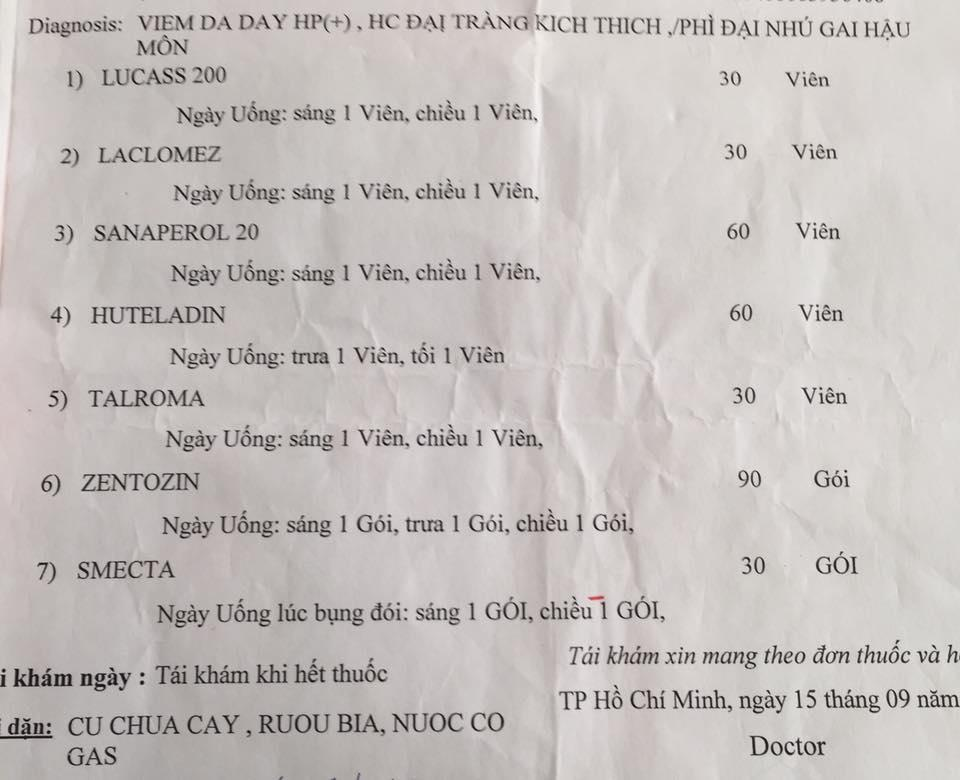
\includegraphics[width=0.7\textwidth]{mep_img/med_extr.png}
\caption{Ví dụ về đơn thuốc, với nội dung bên trong thông thường đều theo một bố cục với quy luật nhất định. Các tên thuốc được liệt kê theo từng hàng, từ trên xuống dưới, với bên trái đang được đánh số thứ tự.}\label{med_extr}
\end{figure}

Thông thường, đơn thuốc cũng giống như các loại hóa đơn, đó chính là bố cục của đơn thuốc sẽ tuân theo một cấu trúc hoặc bán cấu trúc nào đó. Danh sách các tên thuốc trong một đơn thường được trình bày theo một trình tự cố định nhằm giúp bệnh nhân và bác sĩ quan sát dễ hơn. Hình ~\ref{med_expr} biểu diễn một mẫu đơn thuốc cụ thể. Vì thế ta có thể dựa vào mẫu này để trích xuất các từ hay cụm từ có khả năng cao là tên thuốc ra khỏi tập ban đầu bằng các luật (heuristic rules), chúng tôi gói gọn tập luật này vào trong một bước gọi là \textbf{Medicine Extractor}.

Nhờ vào quan sát trên, ta có thể phân loại các đơn thuốc ra làm hai nhóm chính, sau đó tiến hành tách tên thuốc tiềm năng ra khỏi đơn thuốc thông qua một tập các Regular Expression:


\begin{itemize}

\item[-] Luật 01. \textbf{^([0-9]+)(?:\textbackslash.|\textbackslash,)* *(?:(.*?) *\textbackslash((.*?)\textbackslash)*|(.*?) *\\\textbackslash((.*)|(.*)|(\textbackslash(.*?\textbackslash)))}. Theo trường hợp này, mỗi tên thuốc sẽ nằm trên một dòng và có số thứ tự đứng trước. Trên dòng đó, ngoài tên thuốc thì cũng đi kèm với hoạt chất nằm chung (vị trí của tên thuốc và hoạt chất có thể hoán đổi cho nhau tùy đơn thuốc, tuy nhiên vẫn đảm bảo thành phần liền sau sẽ nằm trong dấu ngoặc đơn. Với luật này, ta có thể trích xuất được một lượng tối thiểu các tên thuốc ra khỏi đơn thuốc, đồng thời khả năng chúng là tên thuốc cũng cao nhất, vì hầu hết chỉ dòng chứa tên thuốc mới có nhu cầu có số đứng trước. Hình ~\ref{med_extr_rule_1} chỉ ra một mẫu đơn thuốc thuộc luật 1.

\begin{figure}
\centering
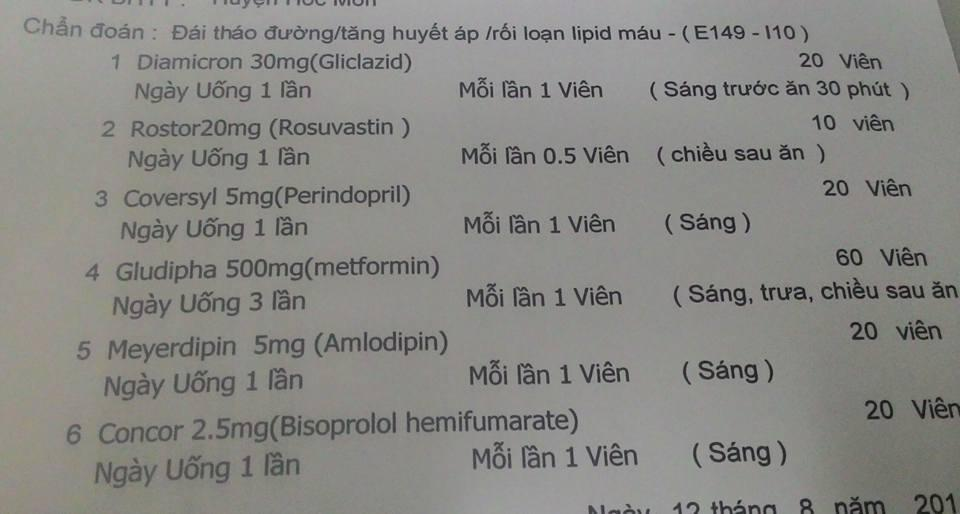
\includegraphics[width=0.8\textwidth]{mep_img/med_extr_rule_1.png}
\caption{Mẫu đơn thuốc có dạng như luật 01 đề cập khi dùng Medicine Extractor.}\label{med_extr_rule_1}
\end{figure}

\item[-] Luật 02. \textbf{^(?:(?!(?:\textbackslash(| ))(.+?) *\textbackslash(+([^)\textbackslash n\textbackslash r]+)\textbackslash)*)}. Luật này cũng tương tự như luật đầu tiên, tuy nhiên bỏ bớt đi điều hiện là phải có số đứng trước. Bằng cách này, ta có thể xử lý được thêm cả những dòng chứa thuốc mà không có số thứ tự. Luật này tuy sẽ làm tăng số dòng nhận được, tuy nhiên vẫn sẽ đảm bảo hiệu suất mô hình, đồng thời là bước dự phòng khi OCR vì vấn đề nào đó mà không thể nhận diện được số thứ tự đứng trước tên thuốc. Hình ~\ref{med_extr_rule_2} đề cập đến một ví dụ cho trường hợp đơn thuốc tuân theo luật 2.

\begin{figure}
\centering
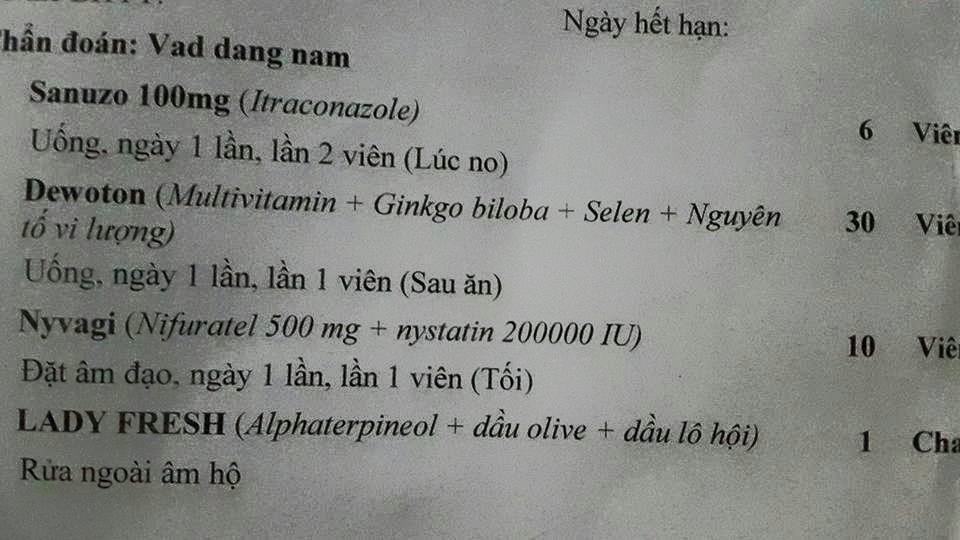
\includegraphics[width=0.7\textwidth]{mep_img/med_extr_rule_2.png}
\caption{Mẫu đơn thuốc có dạng như luật 02, không có số thứ tự đứng đầu.}\label{med_extr_rule_2}
\end{figure}

\item[-] Ngoài ra, có một số ít mẫu đơn thuốc có dạng tên thuốc và hoạt chất nằm trên nhiều dòng. Tuy nhiên trường hợp này ít xảy ra nên khóa luận không tập trung vào để đảm bảo hiệu năng của mô hình. Hình ~\ref{med_extr_rule_3} thể hiện một trường hợp rõ nét nhất cho một đơn thuốc không thuộc phạm vi quản lý của \codeword{MEP}.

\begin{figure}
\centering
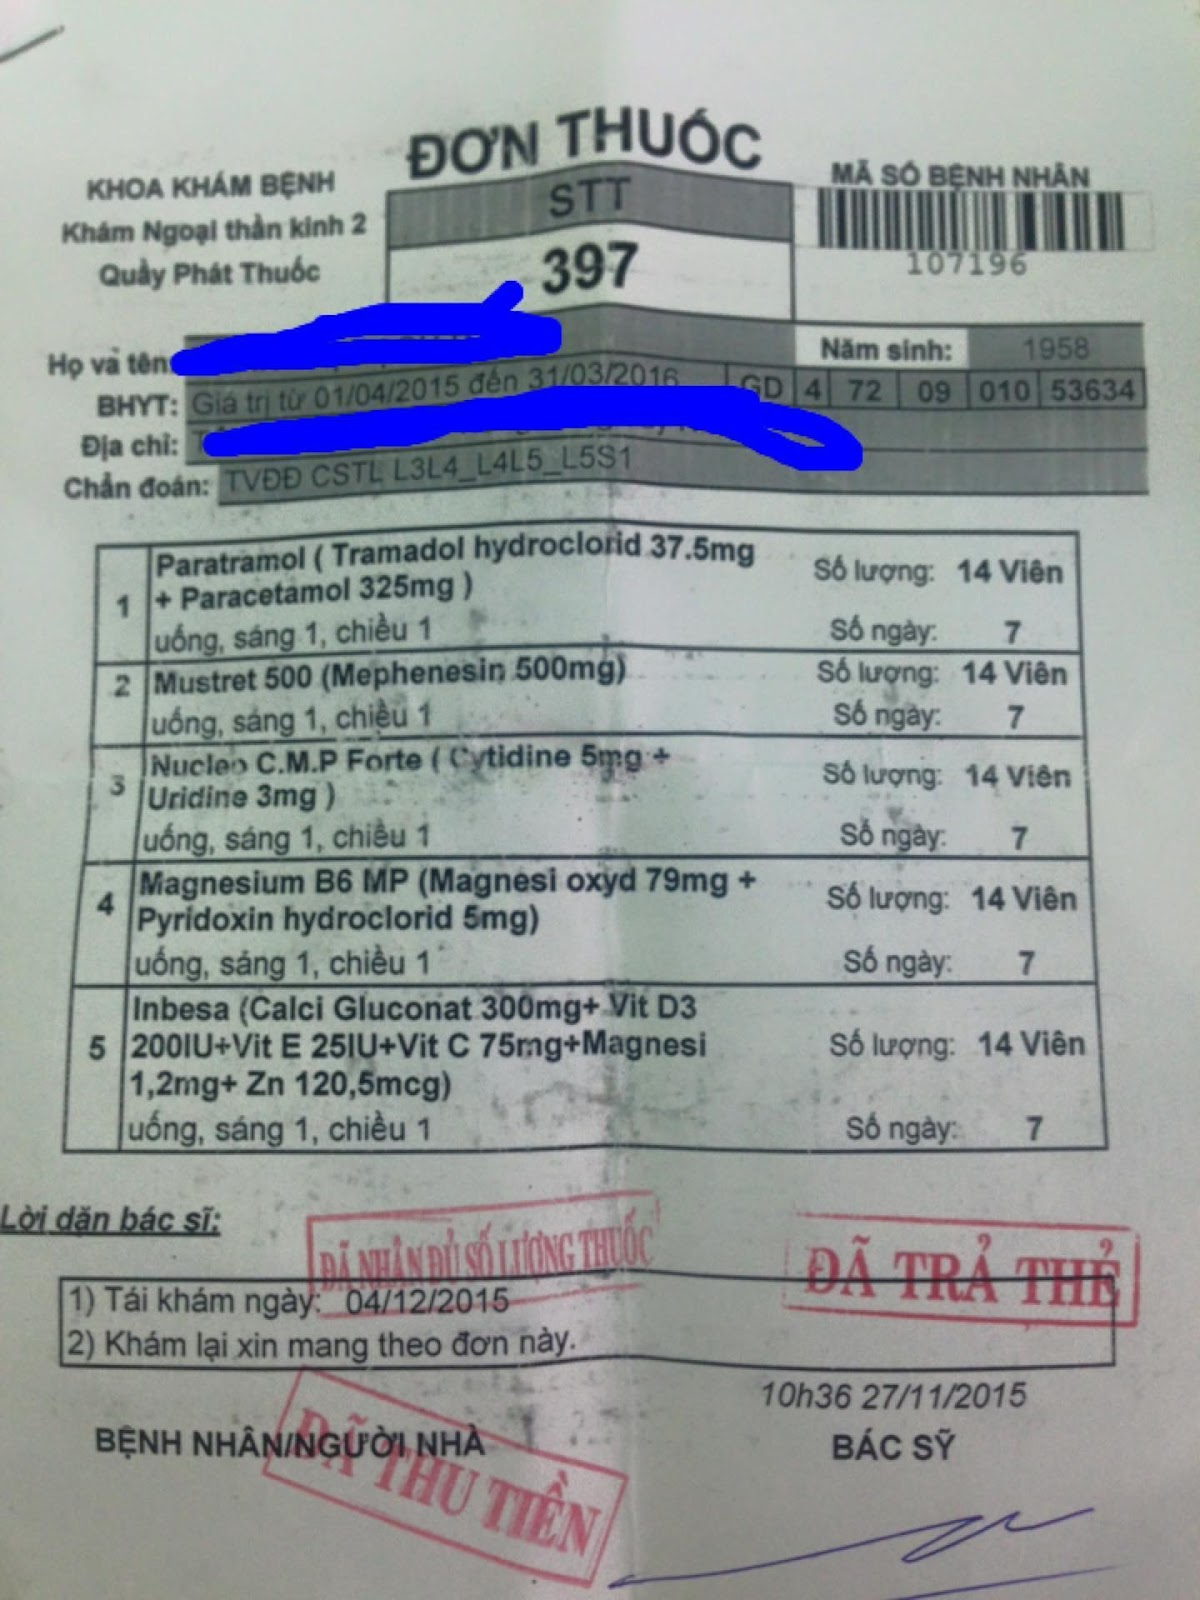
\includegraphics[width=0.7\textwidth]{mep_img/med_extr_rule_3.png}
\caption{Mẫu đơn thuốc không có dạng đặc biệt, khi tên thuốc và hoạt chất nằm trên cùng một dòng nhưng giao diện in lại có cắt dòng dẫn đến có thể có 2 dòng cho mỗi dòng thuốc.}\label{med_extr_rule_3}
\end{figure}

\end{itemize}

\section{MergeOCR}

Để việc trích xuất dựa trên Regex hoạt động tốt, các dòng chứa tên thuốc cần được phát hiện và đóng khung đầy đủ các thành phần cần thiết. Tuy nhiên, do hình ảnh có thể bị mờ, nhiễu khiến cho thuật toán OCR có thể không thực hiện tốt. Nghĩa là thay vì các vùng phát hiện được kỳ vọng chứa tất cả chữ số, tên thuốc và thành phần thuốc thì kết quả nhận được là tập hợp nhiều bounding box chứa các thành phần riêng lẻ giống như trong hình ~\ref{mergeocr_1}. Hậu quả là hệ thống Medicine Extractor được mô tả phía trên sẽ không thực hiện được hiệu quả do không khớp với biểu thức RegEx.

Nhằm khắc phục vấn đề, chúng tôi đề xuất một bước mở rộng tên là MergeOCR. Mục đích của bước này là tìm cách gom các văn bản của các bounding box trên cùng một dòng thành một dòng văn bản duy nhất. Ngoài việc một dòng bị tách thành các bounding box khác nhau, chúng tôi còn gặp phải vấn đề là ranh giới giữa các bounding box này có thể không tách biệt rõ ràng. Trong một vài trường hợp, các khung được phát hiện trong hình ảnh đơn thuốc nằm chồng chéo lên nhau, dẫn đến ta hay lầm tưởng rằng chúng đang nằm cùng trên một dòng. Vì thế, thuật toán đề xuất cần cải thiện tốt cả hai khía cạnh này.

\begin{figure}
\centering
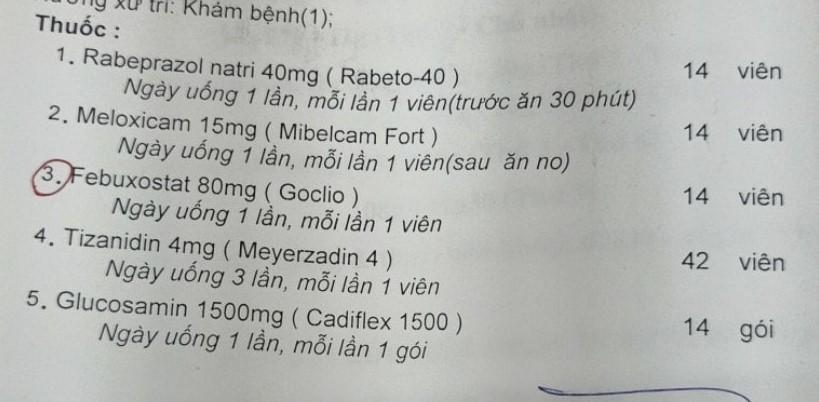
\includegraphics[width=0.7\textwidth]{mep_img/mergeocr_1.png}
\caption{Mẫu đơn thuốc bị méo khiến cho các bounding box của bước phát hiện văn bản bị chồng chất lên nhau, không được coi là một hàng độc lập.}\label{mergeocr_1}
\end{figure}

Chúng tôi đề xuất sử dụng thuật toán Agglomerative Hierarchical Clustering (AHC) cho việc gom nhóm các khung trên cùng một dòng về lại thành một nhóm duy nhất. Thuật toán AHC có ưu điểm là đơn giản, không cần xác định trước số nhóm cần gom cụm. Trong trường hợp này, ban đầu tất cả các bounding box sẽ được đưa vào một nhóm riêng tương ứng. Sau đó thuật toán sẽ lặp trên toàn bộ các nhóm để tiến hành gom nhóm lại. 

Để tính được khoảng cách giữa 2 input (2 bounding box), chúng tôi định nghĩa D(a, b) là khoảng cách giữa 2 node a và b, bằng khoảng cách giữa 2 tọa độ trục y của 2 điểm là tâm của 2 node a b tương ứng, được tính trong công thức ~\ref{eq:AHC_DIST}.

\begin{dmath}
    \label{eq:AHC_DIST}
    \text{DISTANCE(a, b) = } | center_y^a - center_y^b |
\end{dmath}

Trong đó, tâm của input a chính là trọng tâm của bounding box A, hay còn gọi là \textit{center_of_mass}, được ví dụ như trong hình ~\ref{center_of_mass}. Mỗi điểm ảnh trong A sẽ có khối lượng khác nhau (hay còn gọi là độ sáng tại điểm ảnh đó), vì thế ảnh hưởng của nó tới văn bản bên trong cũng khác nhau. Một bounding box có trọng tâm lệch về phía dưới cũng sẽ có phần văn bản lệch về phía dưới. Với cách tính như vậy thì ta luôn có thể ưu tiên chỉ tính toán vị trí tương đối của một khung chứa văn bản thông qua một điểm, không cần quan tâm việc OCR có cắt sát tối ưu hay không. 

\begin{figure}
\centering
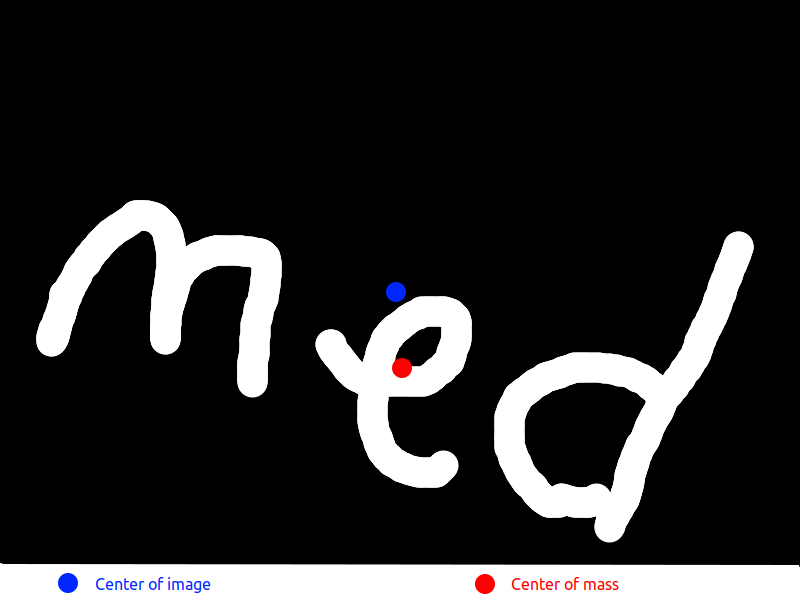
\includegraphics[width=0.6\textwidth]{mep_img/center_of_mass.png}
\caption{Trọng tâm của một hình ảnh còn dựa vào khôi lượng tại mỗi điểm ảnh bên trong.}\label{center_of_mass}
\end{figure}

Sau khi có công thức tính toán khoảng cách giữa 2 node, ta sẽ tiếp tục sử dụng Average-Linkage để tính toán khoảng cách giữa 2 cụm với nhau. Average-Linkage sẽ tính toán trung bình khoảng cách từ mỗi bounding box từ cụm này tới các node tương ứng trong cụm bên kia theo công thức trong ~\ref{eq:Average_Linkage}.

\begin{dmath}
    \label{eq:Average_Linkage}
    \text{DIST_AVG(} {\{x_n\}}_{n=1}^N, {\{y_m\}}_{m=1}^M \text{)} = \frac{1}{NM}\sum_{n=1}^{N}\sum_{m=1}^{M} ||x_n - y_m ||
\end{dmath}

Để đảm bảo gom cụm đạt hiệu quả về cả thời gian cũng như chất lượng, chúng tôi thực hiện nâng cấp bằng cách cắt tỉa thuật toán thông qua một ngưỡng threshold. Threshold này yêu cầu khoảng cách giữa 2 cụm không được lớn hơn, dẫn đến hệ quả là 2 bounding box không thuộc cùng một dòng sẽ không bao giờ phải gom lại thành một cụm, đồng thời kết thúc sớm thuật toán và trả ra kết quả. MergeOCR được thực hiện sau khi nhận dạng văn bản bằng OCR, cho nên các bounding box nằm trên 1 dòng vẫn được nhận dạng riêng biệt, và giúp cho việc nhận dạng của VietOCR đạt hiệu quả hơn, tránh bị nhiễu.

Thuật toán ~\ref{alg:AHC} mô tả chi tiết phiên bản AHC do chúng tôi đề xuất và tối ưu, dựa trên thuật toán gốc tại \cite{day1984efficient}.

\begin{algorithm}[H]
    \caption{Agglomerative Hierarchical Clustering} \label{alg:AHC}
    \begin{algorithmic}[1]
        \State \textbf{Input: } Vector trọng tâm của các bounding box $\{ x_n \}_{n=1}^{N}$, ma trận khoảng cách giữa các cluster $DIST(G_1, G_2)$ tương ứng.
        \State \textbf{Input 2: } $\varepsilon \ gets threshold$ \Comment{Threshold quy định ngưỡng để coi 2 input nằm trên cùng dòng.}
        \State Khởi tạo $A \gets \emptyset$.
        \For{$n \gets 1...N $}
            \State $A \gets A \cup \{\{x_n\}\}$ \Comment{Khởi tạo mỗi nhóm sẽ chứa một bounding box}
        \EndFor
        
        \State $T \gets A$ \Comment{Khởi tạo cây lưu kết quả merge.}
        \State $D_{min} = +\infty$ \Comment{khởi tạo khoảng cách nhỏ nhất giữa hai input.}
        
        \While{$|A| > 1$ \textbf{and} $D_{min} > \varepsilon$} \Comment{Lặp cho đến khi tập A chỉ còn 1 phần tử hoặc không merge được nữa do không thỏa ngưỡng.}
                \State $G_1^{*}, G_2^{*} \gets \argmin_{G_1, G_2 \in A; G_1, G_2 \in A}$ $DIST(G_1, G_2)$ \Comment{Tìm ra cặp cluster cũ gần nhau nhất.}
                
                \State $A \gets (A \setminus \{ G_1^* \}) \setminus \{ G_2^* \}$ \Comment{Loại cặp cluster cũ ra khỏi tập tìm input.}
                
                \State $A \gets A \cup \{ G_1^* \cup G_2^* \}$ \Comment{Lưu tập mới tìm được vào tập input.}
                
                \State $T \gets T \cup \{ G_1^* \cup G_2^* \}$ \Comment{Lưu tập mới tìm được vào cây kết quả.}
                
                \State $D_{min} \gets DIST(G_1^*, G_2^*)$ \Comment{Gán lại khoảng cách nhỏ nhất}
        \EndWhile
        
        \State \textbf{Return: } $T$. \Comment{Trả về kết quả các cụm là các dòng trong văn bản.}
        
    \end{algorithmic}
\end{algorithm}

Kết quả của bước này sẽ là nhiều cụm, mỗi cụm có chữa nhiều bounding box, từ đây các văn bản trong cùng một cụm, hay nói cách khác là trên cùng một dòng, sẽ được nối với nhau theo thứ tự từ trái sang phải theo trục X. Văn bản này đáp ứng tốt yêu cầu đầu vào của Medicine Extractor như trong hình ~\ref{merged_img}, từ đó cải thiện toàn bộ hệ thống \codeword{MEP} của chúng tôi.

\begin{figure}
\centering
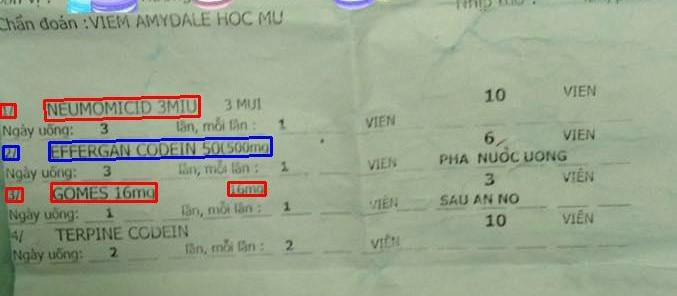
\includegraphics[width=0.7\textwidth]{mep_img/merged_img.png}
\caption{MergeOCR giúp gộp các bounding box trên một dòng lại với nhau.}\label{merged_img}
\end{figure}

\section{Medicine Classifier}

Với sự hỗ trợ từ MergeOCR và Medicine Extractor, ta đã có thể lấy được các tên thuốc tiềm năng, và nhiệm vụ tiếp theo chính là lấy được chính xác tên thuốc trên dòng chứa tên thuốc đó. Thông thường, một dòng chứa tên thuốc có thể chứa nhiều thành phần, bao gồm số thứ tự, tên thuốc, hoạt chất, liều lượng, cách dùng, chỉ định... Đặc biệt, dù đa số đơn thuốc đều có mẫu cố định là có số thứ tự, tuy nhiên về thứ tự giữa tên thuốc và hoạt chất thì lại không có một chuẩn chung. Tên thuốc có thể đứng trước hoạt chất, hoặc ngược lại, thậm chí có trường hợp đơn thuốc không có hoạt chất trong dòng đó. 

Như vậy, cần có một mô hình giúp phân lớp xem một đoạn văn bản có phải là tên thuốc hay không, đồng thời giảm thời gian xử lý toàn bộ dữ liệu đầu vào và giải quyết bài toán một cách chính xác hơn. Đây chính là bài toán phân lớp văn bản (Text Classification) trong lĩnh vực xử lý ngôn ngữ tự nhiên (NLP). Dựa trên ưu điểm đã phân tích của mô hình TCN, chúng tôi sử dụng nó cho \codeword{MEP}, đặt tên là Medicine Classifier, có kiến trúc được mô tả trong hình ~\ref{medicine_classifier_1}.

\begin{figure}
\centering
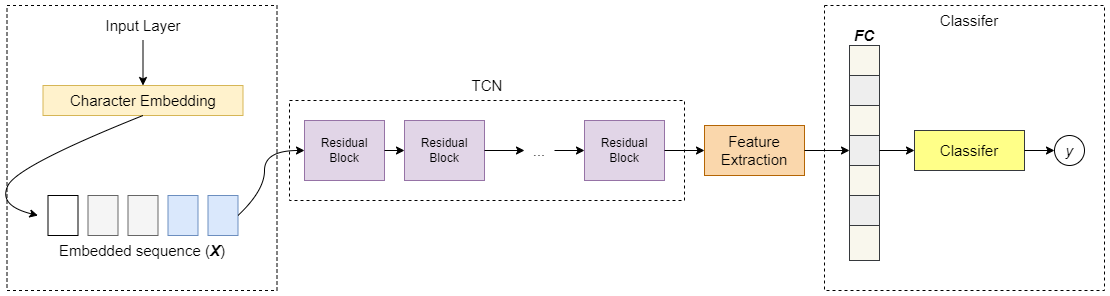
\includegraphics[width=1.0\textwidth]{mep_img/medicine_classifier_1.png}
\caption{Mô hình Medicine Classifier do chúng tôi đề xuất nhằm phân lớp văn bản.}\label{medicine_classifier_1}
\end{figure}

Cấu trúc mô hình bao gồm 2 phần chính, cụ thể như sau. Phần đầu tiên, văn bản đầu vào sẽ được đẩy qua bộ character embedding để chuyển về một chuỗi giá trị (sequence). Sau đó thông qua việc padding với câu dài nhất tại thời điểm huấn luyện nhằm giúp các câu khác nhau đều được biểu diễn về cùng một kích thước. Các giải pháp cho bài toán phân lớp văn thường được ứng dụng cho việc phân lớp nguyên một câu hay cả đoạn văn, bài văn. Vì thế, thông thường người ta hay dùng word embedding để giúp cho mô hình học được ngữ cảnh của văn bản tốt hơn thông qua sự liên kết giữa các từ trong câu. 

Tuy nhiên, đối với tên thuốc, nó thuộc dạng short-text, chỉ cấu tạo từ một đến một vài từ là tối đa. Tên thuốc thường được cấu tạo từ một số các kí tự mà khi ghép lại với nhau thì tỏ ra vô nghĩa, không giống với cách cấu trúc của từ ngữ thông thường. Vì vậy, chúng tôi đề xuất sử dụng character embedding để thay thế cho word embedding. Cách này vừa có thể khắc phục vấn đề , vừa có thể xử lý cả các tên thuốc bị sai cú pháp (misspelling). Thêm nữa, khi dùng character embedding, ta có thể có được một sequence đủ dài đối với cả short-text, từ đó hạn chế được overfitting.

Phần thứ hai là mô hình TCN. Nó giúp ta học được sự liên kết giữa các ký tự trong sequence của character embedding.Việc bị thiếu hay bị sai một kí tự sẽ không ảnh hưởng nhiều đến tổng thể của chuỗi, do vậy nó vẫn đảm bảo hoạt động tốt ngay cả khi tên thuốc bị đánh sai cú pháp. Đồng thời, hiệu năng của TCN đạt được khá tốt. Nó có thể xử lý một lượng lớn input trong một thời gian ngắn. Các feature sau khi qua TCN sẽ được đẩy đến lớp fully connected, với mục tiêu là phân thành 3 lớp cố định. Cụ thể, ta sẽ phân lớp ra thành tên thuốc, hoạt chất và unknown (tức là không thuộc 2 lớp tên thuốc hoặc hoạt chất).

Dữ liệu huấn luyện của Medicine Classifier bao gồm, tên thuốc và hoạt chất được tách riêng từ từ điển thuốc, còn các tên tự do được thu thập từ dữ liệu hỏi đáp trên Yahoo. Tất cả các nhóm input đều được lọc và làm sạch để sao cho có cùng đặc trưng, như là min, mean, median, std, max. Đồng thời, để đảm bảo tất cả đều là short-text, chúng tôi cũng giới hạn số từ trong mỗi input không vượt quá một ngưỡng nhất định là 5 từ, cũng là số từ tối đa của tập dữ liệu các tên thuốc phổ biến. 

Đầu ra của mô hình Medicine Classifier cho mỗi nhãn input chính là một chuỗi các xác suất để phân văn bản đó vào lớp tương ứng. Mô hình sẽ quy định một ngưỡng threshold nhất định để xác định xem nhãn đó gần với lớp nào nhất. Với việc đảm bảo chất lượng của dữ liệu huấn luyện, chúng tôi kì vọng mô hình Medicine Classifier sẽ hoạt động hiệu quả nhằm phân loại chính xác đâu là tên thuốc, đâu là hoạt chất, và loại ra những tên không hợp lệ trước khi tiếp tục đưa vào bước sau.

\section{Context Aware spell correction}

Sau khi đã thực hiện bước Medicine Classifier, ta đã bỏ những dòng nào không chứa các cụm văn bản được phân lớp vào tên thuốc hoặc hoạt chất. Càng ít dòng được giữ lại, thời gian xử lý sẽ càng được rút ngắn, giúp tối ưu hiệu năng cho toàn bộ hệ thống. Tuy nhiên, bởi vì vẫn có sự nhập nhằng giữa tên thuốc và hoạt chất. Như đã đề cập, đôi khi tên thuốc cũng là hoạt chất, và ngược lại. Cụ thể, đôi khi một dòng vừa chứa tên thuốc và hoạt chất, nhưng hệ thống Medicine Classifier có thể phân cả 2 thành tên thuốc, hoặc cả 2 thành hoạt chất. Vì thế, bước cuối cùng này mục tiêu để lọc bỏ, chỉ giữ lại một tên có khả năng cao là tên thuốc nhất.

Bằng cách so sánh mỗi tên với một bộ từ điển được giới hạn trong phạm vi tên thuốc. Chúng tôi thực hiện tìm kiếm mờ dựa trên khoảng cách Levenshtein (Levenshtein Distance \cite{Levenshtein_distance}) nhằm tối ưu chi phí tính toán. Các tên thuốc sẽ được tìm kiếm gần đúng với tên thuốc gần nhất trong bộ từ điển. Công thức tính khoảng cách Levenshtein được mô tả chi tiết trong hình ~\ref{lev_dist}.

\begin{figure}
\centering
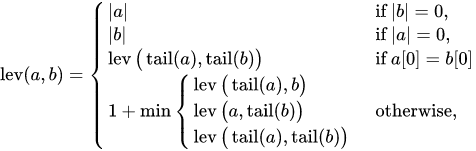
\includegraphics[width=0.7\textwidth]{mep_img/lev_dist.png}
\caption{Công thức tính khoảng cách Levenshtein Distance \cite{Levenshtein_distance}.}\label{lev_dist}
\end{figure}

Về cách cài đặt thuật toán, chúng tôi thực hiện thủ thuật cache lại kết quả cũ để tăng tốc độ tìm kiếm. Chúng tôi chia tập từ điển đơn thuốc ra thành hai, trong đó tập đầu tiên là tập từ điển gốc với kích thước lớn. Khi thực hiện tìm kiếm mờ trên tập này sẽ tốn một lượng thời gian đáng kể. Chính vì vậy chúng tôi sẽ lưu trữ thêm một tập thứ 2 có kích thước nhỏ, chỉ chứa những thuốc thường xuyên được sử dụng bởi hệ thống. Vì tập này có kích thước nhỏ hơn hẳn nên thời gian truy vấn sẽ rất tối ưu, gần như ngay lập tức trả ra kết quả khi có yêu cầu. Hình ~\ref{med_recorrected} chỉ ra một kết quả của đơn thuốc sau khi được trích xuất và sửa lỗi tên thuốc theo như trong từ điển.

\begin{figure}
\centering
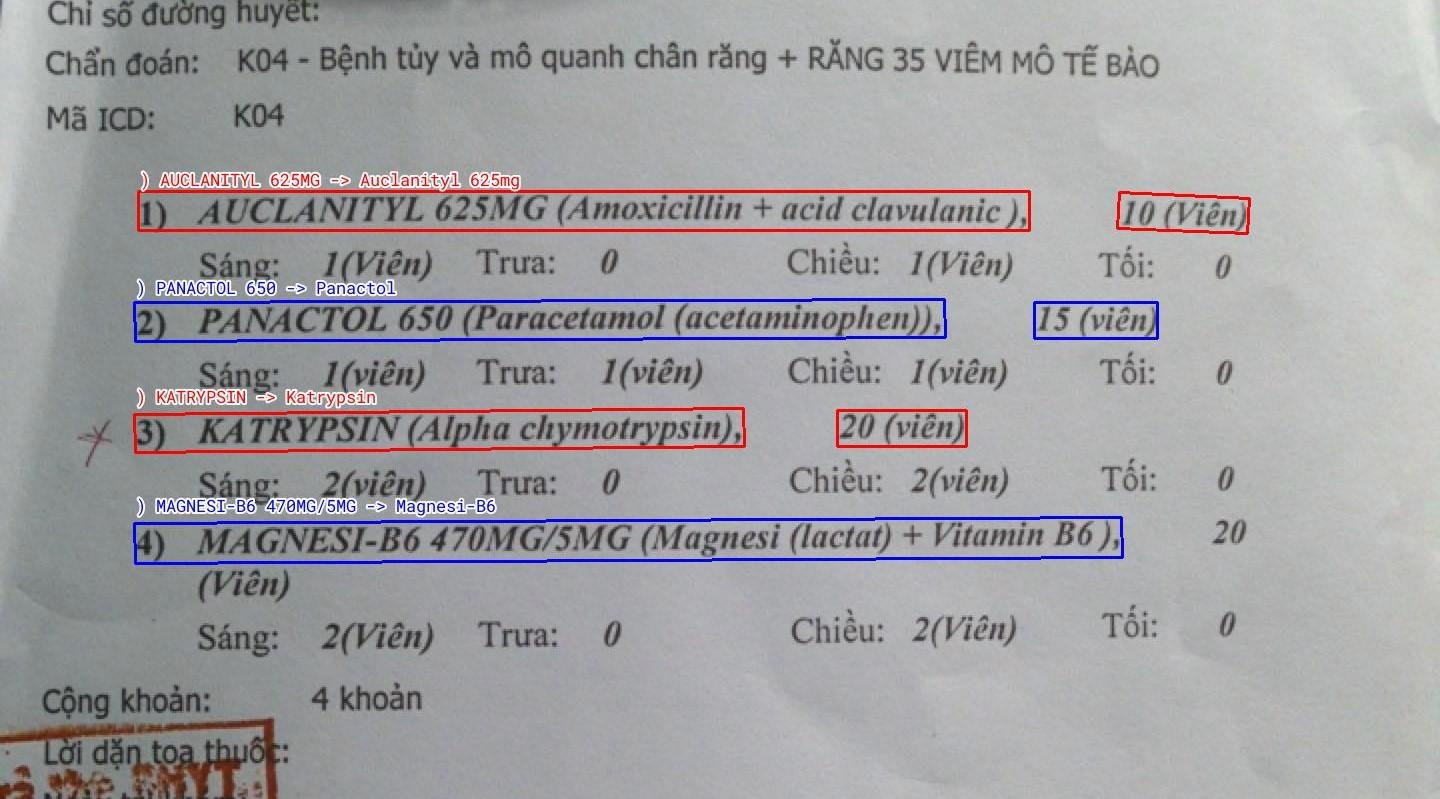
\includegraphics[width=0.7\textwidth]{mep_img/med_recorrected.png}
\caption{Đơn thuốc sau khi trích xuất thông tin tên thuốc và sửa lỗi.}\label{med_recorrected}
\end{figure}

\chapter{Cài đặt thực nghiệm}
\label{Chapter4}

\section{Tập dữ liệu}

Như đã giới thiệu ở trên, đối với bài toán OCR trên hình ảnh đơn thuốc thì những tập dữ liệu văn bản cảnh là chưa đủ để đánh giá khả năng của mô hình. Do vậy, chúng tôi đã thu thập và đề xuất một tập dữ liệu mới bổ sung, có tên là Prescription Dataset nhằm mục đích đánh giá cho các mô hình nhận dạng ảnh đơn thuốc. Trong đó, dữ liệu bao gồm 1543 hình ảnh với hơn 10000 loại thuốc khác nhau. Mỗi tên thuốc được bao quanh bởi một bounding box và được gán nhãn bằng tên thuốc đúng. Tập dữ liệu này được chúng tôi thu thập từ các nguồn như bệnh viện và các trang web chuyên về phân phối thuốc.

Mặc dù ngôn ngữ chính của tập dữ liệu này là tiếng Việt, tuy nhiên tên thuốc thường là tên khoa học nên chúng ít chịu ảnh hưởng bởi dấu câu hoặc ngữ pháp tiếng Việt, tất nhiên chúng tôi cũng thống kê và sử dụng những tên thuốc thuần Việt như "Cao bạch hổ", "Tinh dầu",… Tập dữ liệu này chứa hình ảnh đơn thuốc được chụp lại bằng camera của điện thoại, với độ sáng hoặc góc nghiêng là không cố định.

Những điều kiện trên tuy sẽ giống thực tế, có lợi cho sự tổng quát của mô hình \codeword{MEP}, nhưng cũng vô tình tạo ra những thách thức không hề nhỏ cho mô hình nhận diện, làm thế nào để có thể nhận diện được chính xác văn bản ở những điều kiện khó khăn về độ sáng, góc nghiêng. Do đó, tập dữ liệu này sẽ đóng vai trò là một thang đo thực tế cho hệ thống nhận dạng và trích xuất thông tin thuốc như của chúng tôi. Trong những phần tiếp theo, chúng tôi sẽ mô tả quá trình thu thập cũng như gán nhãn cho bộ dữ liệu.

\subsection{Thu thập dữ liệu}
Phần lớn hình ảnh trong tập dữ liệu của chúng tôi đã được tải xuống từ một group
Facebook có tên là "\textbf{KHO ĐƠN THUỐC}", đây là một group nhỏ được lập ra với mục đích tập
hợp đơn thuốc từ khắp mọi nơi. Bên cạnh đó, một số lượng không hề nhỏ đơn thuốc được
chúng tôi đến những bệnh viện lớn và nhỏ trong khu vực để thu thập. Để đảm bảo không xảy ra hiện tượng trùng lặp, chúng tôi đã thực hiện việc kiểm tra một cách thủ công. Tập dữ
liệu cuối cùng sau khi tinh chỉnh chứa 1051 hình ảnh từ Internet và 492 hình ảnh do các thành viên trong nhóm thu thập từ bệnh viện và chụp lại.
\subsection{Gán nhãn dữ liệu}
Ban đầu, chúng tôi lấy ra một vài hình ảnh để thực hiện quá trình gán nhãn mẫu để ước
lượng ra một quy trình gán nhãn phù hợp với tập dữ liệu. Một bounding box được vẽ bao
quanh những phần văn bản là tên thuốc. Tọa độ và tên thuốc (nhãn) của bounding box sẽ
được lưu lại trong một tập tin văn bản bán cấu trúc (JSON). Sau khi hoàn thành giai đoạn
làm thử trên những hình ảnh ban đầu, các kỹ thuật thống kê được áp dụng để đánh giá kết
quả gán nhãn. Từ đó chúng tôi có được những nhận định sơ bộ về kết quả gán nhãn nhằm
cập nhật qui trình gán nhãn giúp nâng cao chất lượng, sự đồng thuận trong kết quả gán
nhãn.

Sau khi tổng kết giai đoạn làm thử, bước tiếp theo là thực hiện gán nhãn trên tập dữ liệu
1500 hình ảnh. Chúng tôi chia 1500 hình ảnh thành 4 nhóm, mỗi nhóm 375 hình ảnh. Mỗi
hình ảnh được gán nhãn thủ công bởi mỗi thành viên trong nhóm nhằm đảm bảo độ chính
xác của tập dữ liệu trong quá trình thực nghiệm.

\subsection{Bộ dữ liệu từ điển tên thuốc}
Ngoài bộ dữ liệu để thực nghiệm, chúng tôi cũng thu thập thêm nguồn dữ liệu dồi dào tên
thuốc từ Drugbank Việt Nam và thế giới. Với tổng cộng 41.000 nhãn tên thuốc riêng biệt
cùng với hơn 100.000 tên hoạt chất, gấp hơn 100 lần so với bộ dữ liệu cũ trong nghiên cứu của các nhóm khóa luận trước đó, \codeword{MEP} hứa hẹn sẽ cho ra kết quả tốt hơn và ổn định hơn so với mô hình tiền nhiệm.

\section{Cấu hình tham số}

Trong phần này khóa luận sẽ giới thiệu các tham số và thiết bị sử dụng trong quá trình thực nghiệm. Cụ thể, các lần thực nghiệm đều được chúng tôi chạy trên thiết bị có cùng cấu hình gồm chip xử lý là 2 lõi CPU Intel Xenon @2.20GHz, và chip đồ họa là GPU Tesla K80 với CUDA Version 11.2. 

Đối với phần phát hiện văn bản, chúng tôi sử dụng tham số cho CRAFT như sau: \verb|text_threshold = 0.75| và \verb|link_threshold = 0.4|. Đồng thời chúng tôi sử dụng bộ pretrain \verb|craft_mlt_25k| (được train trước với các tập dataset SynthText, IC13, IC17 với ngôn ngữ chủ yếu là tiếng Anh) cho mô hình. Để nhận diện văn bản sử dụng VietOCR, khóa luận chọn phương pháp cài đặt là \verb|Seq2Seq| đồng thời sử dụng bộ pretrained \verb|vgg_seq2seq| cho mô hình. 

Tham số ngưỡng cho MergeOCR được cài đặt là threshold = 0.02, chỉ ra giới hạn khoảng cách tương đối giữa các bounding box để được coi là nằm trên một dòng. Đối với Medicine Classifier, chúng tôi cấu hình tham số \verb|padding_size = 320|, \verb|filter_size k = 2|, độ giãn nở dilation factor \verb|d = [1, 2, 4]|. Ngoài ra ngưỡng để Medicine Classifier đảm bảo rằng một nhãn là tên thuốc được cấu hình là 0.6. Cuối cùng, chúng tôi cấu hình ngưỡng để tìm kiếm tên thuốc trong bộ dữ liệu đơn thuốc và sửa lỗi chúng là 0.85.

\section{Huấn luyện mô hình}

Đối với \codeword{MEP}, chúng tôi lựa chọn huấn luyện một vài công đoạn, và một số công đoạn sẽ dùng lại bộ tham số có sẵn. Về OCR, cả phần phát hiện văn bản dùng CRAFT và nhận dạng văn bản đều dùng cấu hình có sẵn như đã trình bày ở trên. 

Đối với Medicine Extractor, chúng tôi chỉ lựa chọn mẫu để tách tên thuốc ra khỏi dòng thuốc chứ không có nhu cầu huấn luyện. Tương tự với phần sửa lỗi cuối mô hình, chỉ đơn giản là so khớp, tìm kiếm mờ tên thuốc với cơ sở dữ liệu.
Như vậy, trong phần này chúng tôi tập trung giới thiệu phần huấn luyện mô hình cho MergeOCR và Medicine Classifier.

\subsection{Huấn luyện mô hình MergeOCR}

\textbf{AHC} là một mô hình thống kê, vì vậy công đoạn huấn luyện mô hình khá đơn giản. Vì mỗi ảnh có thể có kích thước khác nhau, đồng thời kích thước văn bản bên trong cũng khác biệt. Vì thế, chúng tôi dùng chính dữ liệu của mỗi hình bao gồm các bounding box sau bước phát hiện văn bản làm dữ liệu huấn luyện và trả về kết quả. Bằng cách đó, mô hình có thể áp dụng một ngưỡng threshold duy nhất nhưng vẫn đảm bảo tính linh hoạt cho mọi hình ảnh đầu vào.

Đầu tiên, chúng tôi xây dựng một ma trận khoảng cách giữa các khung văn bản với nhau thông qua khoảng cách giữa các trọng tâm (center of mass), sau đó bộ dữ liệu được tính toán sẵn này sẽ được đưa vào huấn luyện mô hình, trong đó khoảng cách giữa các cụm sẽ được tính bằng công thức Average-Linkage. Sau đó, Các nhóm sẽ được tạo ra tương ứng với một dòng văn bản. Mô hình sẽ thực hiện nối văn bản của các bounding box trên mỗi cột vào lại với nhau và sẵn sàng sử dụng. 

\subsection{Huấn luyện mô hình Medicine Classifier}

Dữ liệu dùng để huấn luyện cho mô hình Medicine Classifier là dữ liệu được chúng tôi thu thập từ Drugbank để lấy tên thuốc và hoạt chất, cũng như từ bộ dữ liệu hỏi đáp Yahoo để lấy nhãn còn lại. Với tổng số hơn 230000 mẫu huấn luyện, chúng tôi tiếp tục thực hiện chuẩn hoá dữ liệu, sau đó chia thành 3 tập $D_{train}$, $D_{validation}$ và $D_{test}$. Sau đó, mỗi mẫu dữ liệu này sẽ được đưa vào Tokenizer theo phương pháp character embedding để tạo ra input cho mô hình. Cuối cùng, kích thước tập $D_{train}$ là (168019, 320) và tập $D_{validation}$ phục vụ cho việc huấn luyện mô hình là (42005, 320) và tập $D_{test}$ để kiểm tra mô hình là (23337, 320).

Chúng tôi huấn luyện mô hình với \verb|batch_size = 50|, mỗi epoch sẽ có 3361 batch nhằm mục đích tăng tốc độ hội tụ mô hình mà vẫn đảm bảo thời gian huấn luyện thấp. Với lượng dữ liệu huấn luyện dồi dào cùng với sự kết hợp của kiến trúc TCN, mô hình Medicine Classifier nhanh chóng hội tụ và chúng tôi lựa chọn bộ tham số tại checkpoint có hàm loss thấp nhất để đưa vào sử dụng cho bài toán phân loại tên thuốc.

\section{Phương pháp đánh giá}

Chúng tôi thực hiện đánh giá mô hình MEP thông qua kết quả khi chạy thực nghiệm trên bộ dữ liệu đơn thuốc kể trên, trong đó ghi lại 3 thông tin: (1) Precision, (2) Recall, (3) H-mean.

\begin{itemize}

\item[(1)] Precision (\verb|P|) là độ đo cho độ tin cậy của mô hình khi thực hiện trích xuất tên thuốc ra khỏi đơn thuốc. Cụ thể, nó chính là tỉ lệ dự đoán đúng tên thuốc trên toàn bộ tên thuốc mà mô hình trả về. Công thức tính precision cho mỗi đơn thuốc được thể hiện ở trong công thức ~\ref{eq:precision}. Để tính precision cho toàn bộ mô hình, ta sẽ lấy trung bình độ đo này cho từng đơn thuốc.

\begin{dmath}
    \label{eq:precision}
    P_{MEP} = \frac{|\{accurate\_drugs\} \cap \{ retrieved\_drugs \}|}{|\{ retrieved\_drugs \}|}
\end{dmath}

\item[(2)] Recall (\verb|R|) được dùng để kiểm định tỉ lệ bỏ sót tên thuốc trong mỗi đơn thuốc mà mô hình cần dự đoán. Công thức ~\ref{eq:recall} chỉ ra công thức tính recall cho mỗi đơn thuốc. Ta dùng trung bình của giá trị recall này trên các đơn thuốc để tính được độ đo trên cho toàn bộ mô hình trên tập dữ liệu.

\begin{dmath}
    \label{eq:recall}
    R_{MEP} = \frac{|\{accurate\_drugs\} \cap \{ retrieved\_drugs \}|}{|\{ accurate\_drugs \}|}
\end{dmath}

\item[(3)] H-mean (\verb|H|), hay còn gọi là \verb|F1-score|, được tính bằng cách lấy trung bình điều hòa của hai giá trị precision và recall. Độ đo này được chúng tôi sử dụng để đánh giá tổng thể chất lượng của mô hình và được tính theo công thức ~\ref{eq:hmean}.

\begin{dmath}
    \label{eq:hmean}
    H_{MEP} = 2 \times \frac{P_{MEP} \times R_{MEP}}{P_{MEP} + R_{MEP}}
\end{dmath}

\end{itemize}

Ngoài 3 độ đo này, khóa luận cũng tiến hành đánh giá mô hình thông qua tiêu chí thời gian. Đối với mỗi bước trong phương pháp đề xuất, chúng tôi sẽ tiến hành đo và đối chiếu với hiệu năng của mô hình cũ được đề xuất tại \cite{nguyen2021developing} tương ứng.


\chapter{Kết quả \& Thảo luận}
\label{Chapter5}

\section{Đánh giá mô hình Medicine Classifier}

Medicine Classifier là một bước quan trọng trong phương pháp đề xuất \codeword{MEP} của chúng tôi. Nếu như nó hoạt động không hiệu quả thì hệ thống nhận diện đơn thuốc cũng sẽ không thể sử dụng được.

Theo như phần huấn luyện mô hình, Medicine Classifier hội tụ nhanh và chỉ trong vòng 20 epoch đã đạt được cực tiểu cho hàm $loss$. Hình ~\ref{tfw_acc}, ~\ref{tfw_loss}, ~\ref{tfw_precision}, ~\ref{tfw_recall} thể hiện kết quả huấn luyện cho mô hình Medicine Classifier, được theo dõi và thống kê bằng TF Watcher \cite{TFWatcher}. 

\begin{figure}
\centering
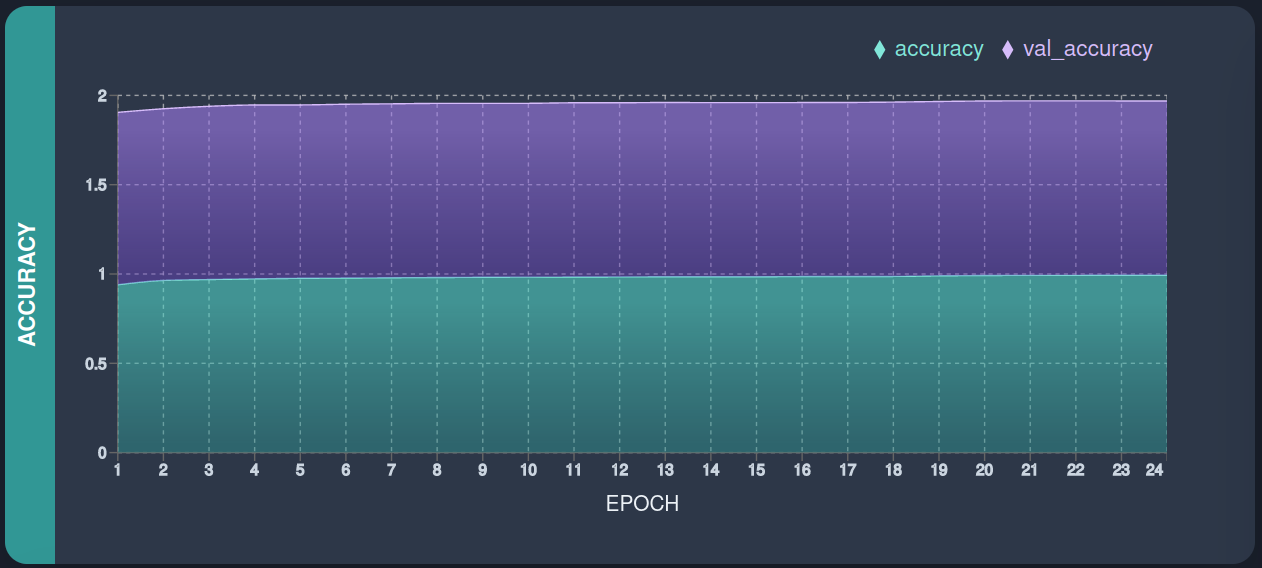
\includegraphics[width=0.8\textwidth]{mep_img/tfw_acc.png}
\caption{Độ chính xác của mô hình Medicine Classifier trong quá trình huấn luyện.}\label{tfw_acc}
\end{figure}

\begin{figure}
\centering
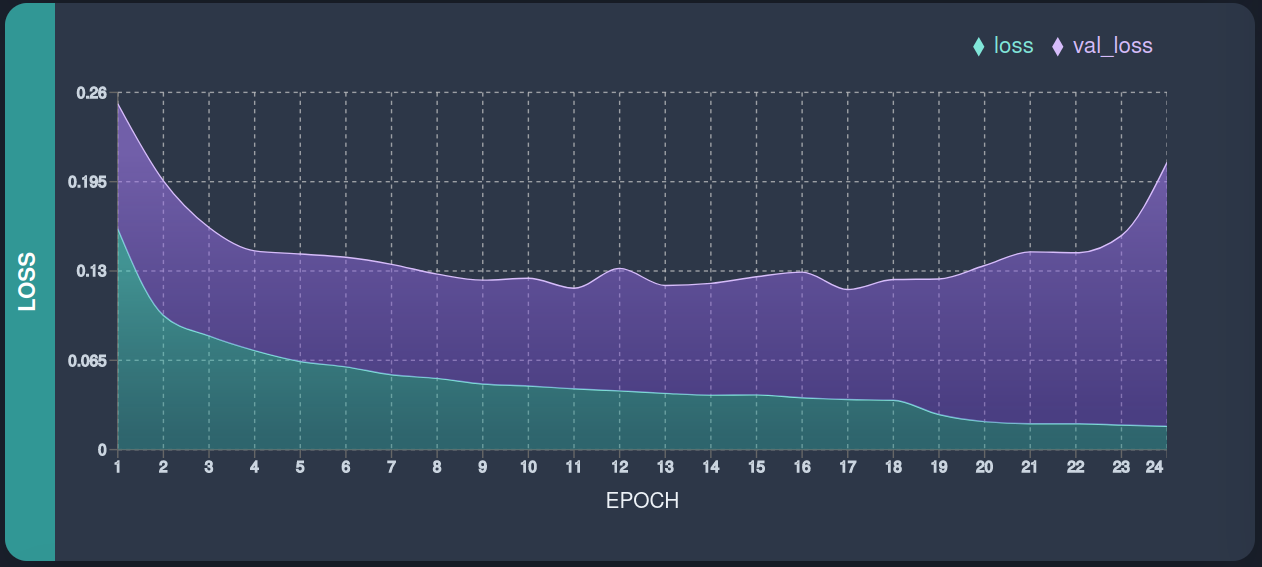
\includegraphics[width=0.8\textwidth]{mep_img/tfw_loss.png}
\caption{Hàm lỗi của mô hình Medicine Classifier trong quá trình huấn luyện.}\label{tfw_loss}
\end{figure}

\begin{figure}
\centering
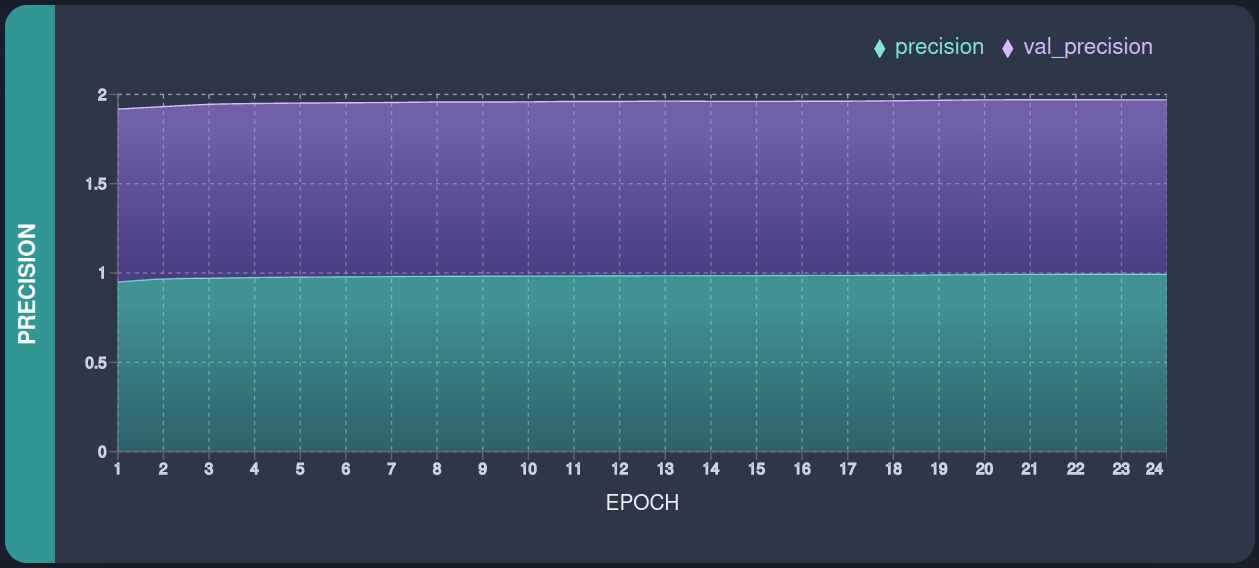
\includegraphics[width=0.8\textwidth]{mep_img/tfw_precision.png}
\caption{Đánh giá mô hình Medicine Classifier bằng độ đo precision trong quá trình huấn luyện.}\label{tfw_precision}
\end{figure}

\begin{figure}
\centering
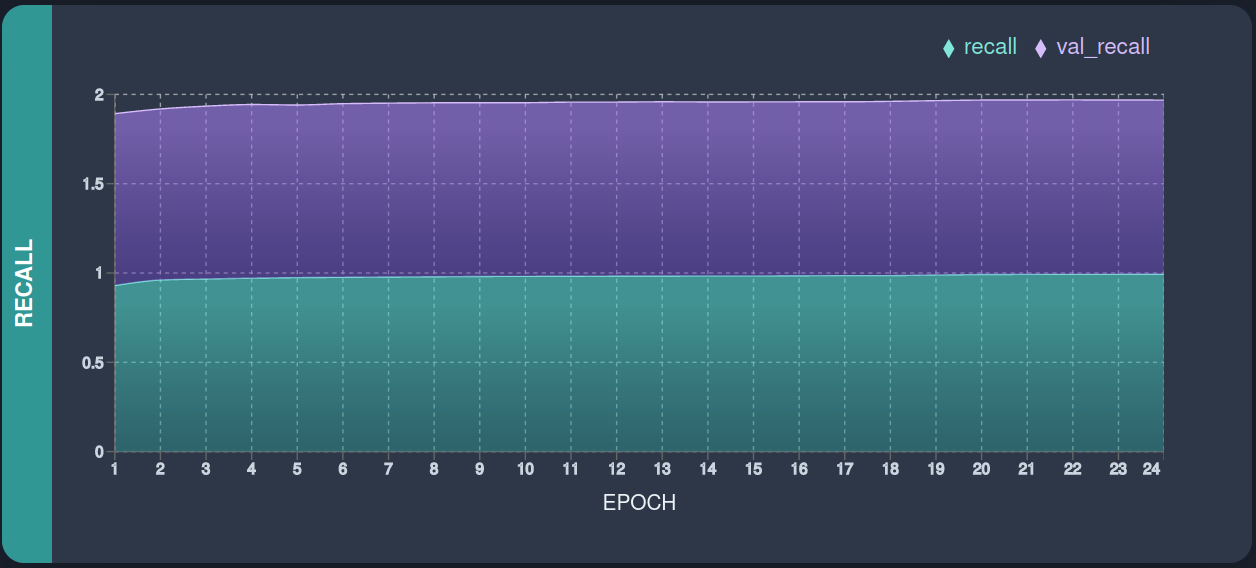
\includegraphics[width=0.8\textwidth]{mep_img/tfw_recall.png}
\caption{Đánh giá mô hình Medicine Classifier bằng độ đo recall trong quá trình huấn luyện.}\label{tfw_recall}
\end{figure}

Từ kết quả trên, ta nhanh chóng nhận ra cả 3 độ đo Accuracy \textit{acc}, Precision \textit{P}, và Recall \textit{R} đều nhanh chóng hội tụ và rất cao, chứng tỏ mô hình này rất phù hợp với bộ dữ liệu cũng như bài toán đặt ra. Các thông số trên đều cao trên $0.95$ khi đánh giá trên cả tập $D_{train}$ lẫn tập $D_{validation}$.

Đối với hàm \textit{loss}, chúng tôi quan sát và thấy rằng ban đầu, cả 2 hàm $L_{train}$ và $L_{validation}$ cho 2 tập đều thấp, với $L_{train} = 0.16$ và $L_{validation} = 0.09$. Những hàm \textit{loss} này giảm dần đều và có sự hoán đổi về mặt giá trị giữa 2 hàm trong trong quá trình huấn luyện mô hình. 

Cực tiểu của hàm $L_{validation}$ là tại \verb|epoch = 11|. Tuy nhiên, khi đến \verb|epoch = 18|, mô hình có dấu hiệu bị overfit, làm $L_{train}$ giảm nhanh nhưng hàm $L_{validation}$ thì lại tăng đáng kể. Vì vậy, chúng tôi chọn checkpoint tốt nhất để sử dụng cho \codeword{MEP} tại epoch bằng 11.

Mô hình Medicine Classifier sau khi được huấn luyện cho kết quả khả quan, đạt $acc_{test} = 0.97$ và $L_{test} = 0.11$ khi đánh giá trên tập ẩn $D_{test}$.

\section{Đánh giá độ chính xác của phương pháp đề xuất MEP}

Chúng tôi thực hiện chạy thử nghiệm trên tập dữ liệu đơn thuốc mà chúng tôi thu thập, được giới thiệu tại mục Chương 4 trên cả hai mô hình, gồm mô hình đề xuất \codeword{MEP} và mô hình tại \cite{nguyen2021developing}.

Bảng ~\ref{exp:tab_1} thể hiện kết quả của \codeword{MEP} so với hệ thống cũ. 

\begin{table}
\centering
\caption{Đánh giá kết quả của hai mô hình nhận dạng đơn thuốc, gồm \textbf{MEP} và \cite{nguyen2021developing}}\label{exp:tab_1}
% \begin{tabular}{|S[table-format=15.0]|S[table-format=10.2]|S[table-format=7.2]|S[table-format=7.2]|}
\begin{tabular}{|c|ccc|}
\hline
Model           & @Precision & @Recall & @H-mean  \\ 
\hline
Method in \cite{nguyen2021developing}      & 0.54       & 0.17    & 0.26     \\ 
\hline
\textbf{MEP} & \textbf{0.94}       & \textbf{0.73}    & \textbf{0.82}     \\
\hline
\end{tabular}
\end{table}

Có thể thấy, các chỉ số độ đo của \codeword{MEP} đều cao hơn hẳn so với mô hình trước đó. Độ đo precision $P_{MEP}$ lên tới \textbf{0.94}, tăng thêm \textbf{0.4} so với phiên bản tiền nhiệm. Điều đó cho thấy, hầu hết trong số các tên thuốc mà mô hình chúng tôi nhận dạng được thì đều đảm bảo độ chính xác. 

Mặc dù thông số recall $R_{MEP}$ tăng rất ấn tượng, cách biệt \textbf{0.54} so với phiên bản tiền nhiệm, tuy nhiên nó mới chỉ đạt \textbf{0.73} cho toàn bộ tập dữ liệu kiểm thử. Điều này có thể là do đầu vào của mô hình bao gồm các đơn thuốc có nhiều nhiễu, dẫn đến OCR chưa lấy được đầy đủ văn bản để mô hình thực hiện trích xuất tên thuốc.

Một nguyên nhân nữa cũng ảnh hưởng đến kết quả của $R_{MEP}$ đó là công đoạn Medicine Extractor vì các tên thuốc tiềm năng được trích xuất ra dựa rất nhiều vào công đoạn này. Mặc dù phần lớn đơn thuốc sẽ thuộc về 2 trường hợp mà chúng tôi đang khai thác, vẫn có một lượng dữ liệu đơn thuốc không theo chuẩn này dẫn đến khó khăn cho mô hình. Điều này hoàn toàn có thể được cải thiện trong những phiên bản tới, khi chúng tôi tăng cường nhiều luật hơn cho Medicine Extractor.

\begin{table}
\centering
\caption{Tầm quan trọng của Medicine Extractor trong hệ thống nhận dạng đơn thuốc}\label{exp:tab_2}
% \begin{tabular}{|S[table-format=15.0]|S[table-format=10.2]|S[table-format=7.2]|S[table-format=7.2]|}
\begin{adjustbox}{angle=-90}
\begin{tabular}{|c|c|c|c|c|}
\hline
Model           & OCRed text & MedicineExtractor & Spell correction & Output \\ 
\hline
Method in \cite{nguyen2021developing}      & Allpovic & - & [Alpovic]@0.9 & Alpovic     \\ 
\textbf{MEP} & Allpovic & \textbf{Allpovic} & [Alpovic]@0.9 & Alpovic     \\
\hline
Method in \cite{nguyen2021developing}      & Eperison 50mg (Macnir) & - & [Macnir]@0.6 & -      \\ 
\textbf{MEP} & Eperison 50mg (Macnir) & \textbf{Macnir} & [Macnir]@1.0 & Macnir     \\
\hline
\textbf{MEP} & Diovan 160mg (Valsartan) & \textbf{Diovan 160mg} & [Diovan 160]@0.94 & Diovan 160     \\
\hline
\end{tabular}
\end{adjustbox}
\end{table}

Ngoài ra, bảng ~\ref{exp:tab_2} cũng chỉ ra tại sao mô hình của chúng tôi hoạt động ổn định hơn phiên bản tiền nhiệm. Chúng tôi giả sử hệ thống OCR làm việc tích cực và cho ra kết quả tương đối chính xác trên cả 2 mô hình, mặc dù điều này là khó đạt được tại mô hình cũ trong bối cảnh sử dụng Tesseract làm bộ nhận dạng văn bản. Đối với văn bản được trích xuất là "Allpovic", cả hai hệ thống trích xuất tên thuốc hoạt động tốt khi độ tin cậy của kết quả trả ra lên tới \textbf{0.9}, mặc dù tên thuốc này đang là sai chính tả.

Tuy nhiên, sự khác biệt bắt đầu xảy ra khi văn bản sau bước OCR là "Eperison 50mg (Macnir)". Việc chỉ so khớp với từ điển thuốc đã khiến cho độ tin cậy của kết quả tại mô hình cũ bị sụt giảm nghiêm trọng, tụt xuống \textbf{0.6}, thấp hơn ngưỡng mà mô hình sử dụng. Điều đó dẫn đến nó không thể phát hiện đây là tên thuốc, và cũng là một trong những nguyên nhân khiến cho \textit{Recall} của mô hình này chỉ đạt 0.17.

\codeword{MEP} có thể giải quyết được vấn đề này một cách triệt để khi Medicine Extractor có thể tách thông tin trong input này ra, một là “Epersion 50mg”, còn lại là "Macnir". "Epersion 50mg" là hoạt chất, nên tất nhiên sẽ được loại bỏ ở những bước phía sau, còn "Macnir" sẽ được đánh dấu là tên thuốc với độ tin cậy tuyệt đối. Tương tự với trường hợp thứ 3, khi thứ tự giữa tên thuốc và hoạt chất trong văn bản sau bước OCR có sự thay đổi, các luật của mô hình chúng tôi vẫn đảm bảo sự ổn định cho kết quả tổng quan của mô hình.

\section{Đánh giá hiệu suất của mô hình}

Ngoài tiêu chí về độ chính xác, thời gian thực thi cũng là một yếu tố quan trọng quyết định đến một mô hình có được ưu tiên sử dụng hay không. Một mô hình với kết quả tuyệt đối nhưng lại mất nhiều thời gian xử lý và tốn nhiều tài nguyên thường không được sử dụng trong thực tế và đem lại giá trị.

Cơ bản, chúng ta cũng biết phần cứng của máy tính mặc dù được mở rộng trong những năm gần đây, tuy nhiên cũng không đủ đáp ứng nếu như không có sự tối ưu đến từ cả hai phía. Mô hình nhận diện tên thuốc do chúng tôi đề xuất được cấu tạo từ nhiều phần, với mỗi phần mang một sứ mệnh khác nhau. Vì vậy, chúng tôi muốn chứng minh rằng các phần này không tỉ lệ thuận với thời gian thực thi và đưa ra kết quả. Cụ thể, kết quả đo lường trên từng công đoạn của mô hình được so sánh và chỉ ra trong hình ~\ref{exp:barchart}.

\begin{figure}
\centering
\scalebox{0.65}{%% Creator: Matplotlib, PGF backend
%%
%% To include the figure in your LaTeX document, write
%%   \input{<filename>.pgf}
%%
%% Make sure the required packages are loaded in your preamble
%%   \usepackage{pgf}
%%
%% Also ensure that all the required font packages are loaded; for instance,
%% the lmodern package is sometimes necessary when using math font.
%%   \usepackage{lmodern}
%%
%% Figures using additional raster images can only be included by \input if
%% they are in the same directory as the main LaTeX file. For loading figures
%% from other directories you can use the `import` package
%%   \usepackage{import}
%%
%% and then include the figures with
%%   \import{<path to file>}{<filename>.pgf}
%%
%% Matplotlib used the following preamble
%%
\begingroup%
\makeatletter%
\begin{pgfpicture}%
\pgfpathrectangle{\pgfpointorigin}{\pgfqpoint{9.000000in}{5.000000in}}%
\pgfusepath{use as bounding box, clip}%
\begin{pgfscope}%
\pgfsetbuttcap%
\pgfsetmiterjoin%
\pgfsetlinewidth{0.000000pt}%
\definecolor{currentstroke}{rgb}{1.000000,1.000000,1.000000}%
\pgfsetstrokecolor{currentstroke}%
\pgfsetstrokeopacity{0.000000}%
\pgfsetdash{}{0pt}%
\pgfpathmoveto{\pgfqpoint{0.000000in}{0.000000in}}%
\pgfpathlineto{\pgfqpoint{9.000000in}{0.000000in}}%
\pgfpathlineto{\pgfqpoint{9.000000in}{5.000000in}}%
\pgfpathlineto{\pgfqpoint{0.000000in}{5.000000in}}%
\pgfpathlineto{\pgfqpoint{0.000000in}{0.000000in}}%
\pgfpathclose%
\pgfusepath{}%
\end{pgfscope}%
\begin{pgfscope}%
\pgfsetbuttcap%
\pgfsetmiterjoin%
\definecolor{currentfill}{rgb}{1.000000,1.000000,1.000000}%
\pgfsetfillcolor{currentfill}%
\pgfsetlinewidth{0.000000pt}%
\definecolor{currentstroke}{rgb}{0.000000,0.000000,0.000000}%
\pgfsetstrokecolor{currentstroke}%
\pgfsetstrokeopacity{0.000000}%
\pgfsetdash{}{0pt}%
\pgfpathmoveto{\pgfqpoint{0.516436in}{0.264771in}}%
\pgfpathlineto{\pgfqpoint{8.887500in}{0.264771in}}%
\pgfpathlineto{\pgfqpoint{8.887500in}{4.750662in}}%
\pgfpathlineto{\pgfqpoint{0.516436in}{4.750662in}}%
\pgfpathlineto{\pgfqpoint{0.516436in}{0.264771in}}%
\pgfpathclose%
\pgfusepath{fill}%
\end{pgfscope}%
\begin{pgfscope}%
\pgfpathrectangle{\pgfqpoint{0.516436in}{0.264771in}}{\pgfqpoint{8.371064in}{4.485891in}}%
\pgfusepath{clip}%
\pgfsetbuttcap%
\pgfsetmiterjoin%
\definecolor{currentfill}{rgb}{0.121569,0.466667,0.705882}%
\pgfsetfillcolor{currentfill}%
\pgfsetlinewidth{0.000000pt}%
\definecolor{currentstroke}{rgb}{0.000000,0.000000,0.000000}%
\pgfsetstrokecolor{currentstroke}%
\pgfsetstrokeopacity{0.000000}%
\pgfsetdash{}{0pt}%
\pgfpathmoveto{\pgfqpoint{0.896939in}{0.264771in}}%
\pgfpathlineto{\pgfqpoint{1.242850in}{0.264771in}}%
\pgfpathlineto{\pgfqpoint{1.242850in}{0.368763in}}%
\pgfpathlineto{\pgfqpoint{0.896939in}{0.368763in}}%
\pgfpathlineto{\pgfqpoint{0.896939in}{0.264771in}}%
\pgfpathclose%
\pgfusepath{fill}%
\end{pgfscope}%
\begin{pgfscope}%
\pgfpathrectangle{\pgfqpoint{0.516436in}{0.264771in}}{\pgfqpoint{8.371064in}{4.485891in}}%
\pgfusepath{clip}%
\pgfsetbuttcap%
\pgfsetmiterjoin%
\definecolor{currentfill}{rgb}{0.121569,0.466667,0.705882}%
\pgfsetfillcolor{currentfill}%
\pgfsetlinewidth{0.000000pt}%
\definecolor{currentstroke}{rgb}{0.000000,0.000000,0.000000}%
\pgfsetstrokecolor{currentstroke}%
\pgfsetstrokeopacity{0.000000}%
\pgfsetdash{}{0pt}%
\pgfpathmoveto{\pgfqpoint{1.885258in}{0.264771in}}%
\pgfpathlineto{\pgfqpoint{2.231170in}{0.264771in}}%
\pgfpathlineto{\pgfqpoint{2.231170in}{4.064071in}}%
\pgfpathlineto{\pgfqpoint{1.885258in}{4.064071in}}%
\pgfpathlineto{\pgfqpoint{1.885258in}{0.264771in}}%
\pgfpathclose%
\pgfusepath{fill}%
\end{pgfscope}%
\begin{pgfscope}%
\pgfpathrectangle{\pgfqpoint{0.516436in}{0.264771in}}{\pgfqpoint{8.371064in}{4.485891in}}%
\pgfusepath{clip}%
\pgfsetbuttcap%
\pgfsetmiterjoin%
\definecolor{currentfill}{rgb}{0.121569,0.466667,0.705882}%
\pgfsetfillcolor{currentfill}%
\pgfsetlinewidth{0.000000pt}%
\definecolor{currentstroke}{rgb}{0.000000,0.000000,0.000000}%
\pgfsetstrokecolor{currentstroke}%
\pgfsetstrokeopacity{0.000000}%
\pgfsetdash{}{0pt}%
\pgfpathmoveto{\pgfqpoint{2.873577in}{0.264771in}}%
\pgfpathlineto{\pgfqpoint{3.219489in}{0.264771in}}%
\pgfpathlineto{\pgfqpoint{3.219489in}{0.633754in}}%
\pgfpathlineto{\pgfqpoint{2.873577in}{0.633754in}}%
\pgfpathlineto{\pgfqpoint{2.873577in}{0.264771in}}%
\pgfpathclose%
\pgfusepath{fill}%
\end{pgfscope}%
\begin{pgfscope}%
\pgfpathrectangle{\pgfqpoint{0.516436in}{0.264771in}}{\pgfqpoint{8.371064in}{4.485891in}}%
\pgfusepath{clip}%
\pgfsetbuttcap%
\pgfsetmiterjoin%
\definecolor{currentfill}{rgb}{0.121569,0.466667,0.705882}%
\pgfsetfillcolor{currentfill}%
\pgfsetlinewidth{0.000000pt}%
\definecolor{currentstroke}{rgb}{0.000000,0.000000,0.000000}%
\pgfsetstrokecolor{currentstroke}%
\pgfsetstrokeopacity{0.000000}%
\pgfsetdash{}{0pt}%
\pgfpathmoveto{\pgfqpoint{3.861896in}{0.264771in}}%
\pgfpathlineto{\pgfqpoint{4.207808in}{0.264771in}}%
\pgfpathlineto{\pgfqpoint{4.207808in}{4.537048in}}%
\pgfpathlineto{\pgfqpoint{3.861896in}{4.537048in}}%
\pgfpathlineto{\pgfqpoint{3.861896in}{0.264771in}}%
\pgfpathclose%
\pgfusepath{fill}%
\end{pgfscope}%
\begin{pgfscope}%
\pgfpathrectangle{\pgfqpoint{0.516436in}{0.264771in}}{\pgfqpoint{8.371064in}{4.485891in}}%
\pgfusepath{clip}%
\pgfsetbuttcap%
\pgfsetmiterjoin%
\definecolor{currentfill}{rgb}{1.000000,0.498039,0.054902}%
\pgfsetfillcolor{currentfill}%
\pgfsetlinewidth{0.000000pt}%
\definecolor{currentstroke}{rgb}{0.000000,0.000000,0.000000}%
\pgfsetstrokecolor{currentstroke}%
\pgfsetstrokeopacity{0.000000}%
\pgfsetdash{}{0pt}%
\pgfpathmoveto{\pgfqpoint{1.242850in}{0.264771in}}%
\pgfpathlineto{\pgfqpoint{1.588762in}{0.264771in}}%
\pgfpathlineto{\pgfqpoint{1.588762in}{0.569467in}}%
\pgfpathlineto{\pgfqpoint{1.242850in}{0.569467in}}%
\pgfpathlineto{\pgfqpoint{1.242850in}{0.264771in}}%
\pgfpathclose%
\pgfusepath{fill}%
\end{pgfscope}%
\begin{pgfscope}%
\pgfpathrectangle{\pgfqpoint{0.516436in}{0.264771in}}{\pgfqpoint{8.371064in}{4.485891in}}%
\pgfusepath{clip}%
\pgfsetbuttcap%
\pgfsetmiterjoin%
\definecolor{currentfill}{rgb}{1.000000,0.498039,0.054902}%
\pgfsetfillcolor{currentfill}%
\pgfsetlinewidth{0.000000pt}%
\definecolor{currentstroke}{rgb}{0.000000,0.000000,0.000000}%
\pgfsetstrokecolor{currentstroke}%
\pgfsetstrokeopacity{0.000000}%
\pgfsetdash{}{0pt}%
\pgfpathmoveto{\pgfqpoint{2.231170in}{0.264771in}}%
\pgfpathlineto{\pgfqpoint{2.577081in}{0.264771in}}%
\pgfpathlineto{\pgfqpoint{2.577081in}{0.658542in}}%
\pgfpathlineto{\pgfqpoint{2.231170in}{0.658542in}}%
\pgfpathlineto{\pgfqpoint{2.231170in}{0.264771in}}%
\pgfpathclose%
\pgfusepath{fill}%
\end{pgfscope}%
\begin{pgfscope}%
\pgfpathrectangle{\pgfqpoint{0.516436in}{0.264771in}}{\pgfqpoint{8.371064in}{4.485891in}}%
\pgfusepath{clip}%
\pgfsetbuttcap%
\pgfsetmiterjoin%
\definecolor{currentfill}{rgb}{1.000000,0.498039,0.054902}%
\pgfsetfillcolor{currentfill}%
\pgfsetlinewidth{0.000000pt}%
\definecolor{currentstroke}{rgb}{0.000000,0.000000,0.000000}%
\pgfsetstrokecolor{currentstroke}%
\pgfsetstrokeopacity{0.000000}%
\pgfsetdash{}{0pt}%
\pgfpathmoveto{\pgfqpoint{3.219489in}{0.264771in}}%
\pgfpathlineto{\pgfqpoint{3.565401in}{0.264771in}}%
\pgfpathlineto{\pgfqpoint{3.565401in}{1.040398in}}%
\pgfpathlineto{\pgfqpoint{3.219489in}{1.040398in}}%
\pgfpathlineto{\pgfqpoint{3.219489in}{0.264771in}}%
\pgfpathclose%
\pgfusepath{fill}%
\end{pgfscope}%
\begin{pgfscope}%
\pgfpathrectangle{\pgfqpoint{0.516436in}{0.264771in}}{\pgfqpoint{8.371064in}{4.485891in}}%
\pgfusepath{clip}%
\pgfsetbuttcap%
\pgfsetmiterjoin%
\definecolor{currentfill}{rgb}{1.000000,0.498039,0.054902}%
\pgfsetfillcolor{currentfill}%
\pgfsetlinewidth{0.000000pt}%
\definecolor{currentstroke}{rgb}{0.000000,0.000000,0.000000}%
\pgfsetstrokecolor{currentstroke}%
\pgfsetstrokeopacity{0.000000}%
\pgfsetdash{}{0pt}%
\pgfpathmoveto{\pgfqpoint{4.207808in}{0.264771in}}%
\pgfpathlineto{\pgfqpoint{4.553720in}{0.264771in}}%
\pgfpathlineto{\pgfqpoint{4.553720in}{1.863732in}}%
\pgfpathlineto{\pgfqpoint{4.207808in}{1.863732in}}%
\pgfpathlineto{\pgfqpoint{4.207808in}{0.264771in}}%
\pgfpathclose%
\pgfusepath{fill}%
\end{pgfscope}%
\begin{pgfscope}%
\pgfpathrectangle{\pgfqpoint{0.516436in}{0.264771in}}{\pgfqpoint{8.371064in}{4.485891in}}%
\pgfusepath{clip}%
\pgfsetbuttcap%
\pgfsetmiterjoin%
\definecolor{currentfill}{rgb}{1.000000,0.498039,0.054902}%
\pgfsetfillcolor{currentfill}%
\pgfsetlinewidth{0.000000pt}%
\definecolor{currentstroke}{rgb}{0.000000,0.000000,0.000000}%
\pgfsetstrokecolor{currentstroke}%
\pgfsetstrokeopacity{0.000000}%
\pgfsetdash{}{0pt}%
\pgfpathmoveto{\pgfqpoint{5.196128in}{0.264771in}}%
\pgfpathlineto{\pgfqpoint{5.542039in}{0.264771in}}%
\pgfpathlineto{\pgfqpoint{5.542039in}{0.388995in}}%
\pgfpathlineto{\pgfqpoint{5.196128in}{0.388995in}}%
\pgfpathlineto{\pgfqpoint{5.196128in}{0.264771in}}%
\pgfpathclose%
\pgfusepath{fill}%
\end{pgfscope}%
\begin{pgfscope}%
\pgfpathrectangle{\pgfqpoint{0.516436in}{0.264771in}}{\pgfqpoint{8.371064in}{4.485891in}}%
\pgfusepath{clip}%
\pgfsetbuttcap%
\pgfsetmiterjoin%
\definecolor{currentfill}{rgb}{1.000000,0.498039,0.054902}%
\pgfsetfillcolor{currentfill}%
\pgfsetlinewidth{0.000000pt}%
\definecolor{currentstroke}{rgb}{0.000000,0.000000,0.000000}%
\pgfsetstrokecolor{currentstroke}%
\pgfsetstrokeopacity{0.000000}%
\pgfsetdash{}{0pt}%
\pgfpathmoveto{\pgfqpoint{6.184447in}{0.264771in}}%
\pgfpathlineto{\pgfqpoint{6.530359in}{0.264771in}}%
\pgfpathlineto{\pgfqpoint{6.530359in}{0.264804in}}%
\pgfpathlineto{\pgfqpoint{6.184447in}{0.264804in}}%
\pgfpathlineto{\pgfqpoint{6.184447in}{0.264771in}}%
\pgfpathclose%
\pgfusepath{fill}%
\end{pgfscope}%
\begin{pgfscope}%
\pgfpathrectangle{\pgfqpoint{0.516436in}{0.264771in}}{\pgfqpoint{8.371064in}{4.485891in}}%
\pgfusepath{clip}%
\pgfsetbuttcap%
\pgfsetmiterjoin%
\definecolor{currentfill}{rgb}{1.000000,0.498039,0.054902}%
\pgfsetfillcolor{currentfill}%
\pgfsetlinewidth{0.000000pt}%
\definecolor{currentstroke}{rgb}{0.000000,0.000000,0.000000}%
\pgfsetstrokecolor{currentstroke}%
\pgfsetstrokeopacity{0.000000}%
\pgfsetdash{}{0pt}%
\pgfpathmoveto{\pgfqpoint{7.172766in}{0.264771in}}%
\pgfpathlineto{\pgfqpoint{7.518678in}{0.264771in}}%
\pgfpathlineto{\pgfqpoint{7.518678in}{0.356353in}}%
\pgfpathlineto{\pgfqpoint{7.172766in}{0.356353in}}%
\pgfpathlineto{\pgfqpoint{7.172766in}{0.264771in}}%
\pgfpathclose%
\pgfusepath{fill}%
\end{pgfscope}%
\begin{pgfscope}%
\pgfpathrectangle{\pgfqpoint{0.516436in}{0.264771in}}{\pgfqpoint{8.371064in}{4.485891in}}%
\pgfusepath{clip}%
\pgfsetbuttcap%
\pgfsetmiterjoin%
\definecolor{currentfill}{rgb}{1.000000,0.498039,0.054902}%
\pgfsetfillcolor{currentfill}%
\pgfsetlinewidth{0.000000pt}%
\definecolor{currentstroke}{rgb}{0.000000,0.000000,0.000000}%
\pgfsetstrokecolor{currentstroke}%
\pgfsetstrokeopacity{0.000000}%
\pgfsetdash{}{0pt}%
\pgfpathmoveto{\pgfqpoint{8.161085in}{0.264771in}}%
\pgfpathlineto{\pgfqpoint{8.506997in}{0.264771in}}%
\pgfpathlineto{\pgfqpoint{8.506997in}{0.959016in}}%
\pgfpathlineto{\pgfqpoint{8.161085in}{0.959016in}}%
\pgfpathlineto{\pgfqpoint{8.161085in}{0.264771in}}%
\pgfpathclose%
\pgfusepath{fill}%
\end{pgfscope}%
\begin{pgfscope}%
\pgfsetbuttcap%
\pgfsetroundjoin%
\definecolor{currentfill}{rgb}{0.000000,0.000000,0.000000}%
\pgfsetfillcolor{currentfill}%
\pgfsetlinewidth{0.803000pt}%
\definecolor{currentstroke}{rgb}{0.000000,0.000000,0.000000}%
\pgfsetstrokecolor{currentstroke}%
\pgfsetdash{}{0pt}%
\pgfsys@defobject{currentmarker}{\pgfqpoint{0.000000in}{-0.048611in}}{\pgfqpoint{0.000000in}{0.000000in}}{%
\pgfpathmoveto{\pgfqpoint{0.000000in}{0.000000in}}%
\pgfpathlineto{\pgfqpoint{0.000000in}{-0.048611in}}%
\pgfusepath{stroke,fill}%
}%
\begin{pgfscope}%
\pgfsys@transformshift{1.242850in}{0.264771in}%
\pgfsys@useobject{currentmarker}{}%
\end{pgfscope}%
\end{pgfscope}%
\begin{pgfscope}%
\definecolor{textcolor}{rgb}{0.000000,0.000000,0.000000}%
\pgfsetstrokecolor{textcolor}%
\pgfsetfillcolor{textcolor}%
\pgftext[x=1.242850in,y=0.167548in,,top]{\color{textcolor}\rmfamily\fontsize{10.000000}{12.000000}\selectfont detection}%
\end{pgfscope}%
\begin{pgfscope}%
\pgfsetbuttcap%
\pgfsetroundjoin%
\definecolor{currentfill}{rgb}{0.000000,0.000000,0.000000}%
\pgfsetfillcolor{currentfill}%
\pgfsetlinewidth{0.803000pt}%
\definecolor{currentstroke}{rgb}{0.000000,0.000000,0.000000}%
\pgfsetstrokecolor{currentstroke}%
\pgfsetdash{}{0pt}%
\pgfsys@defobject{currentmarker}{\pgfqpoint{0.000000in}{-0.048611in}}{\pgfqpoint{0.000000in}{0.000000in}}{%
\pgfpathmoveto{\pgfqpoint{0.000000in}{0.000000in}}%
\pgfpathlineto{\pgfqpoint{0.000000in}{-0.048611in}}%
\pgfusepath{stroke,fill}%
}%
\begin{pgfscope}%
\pgfsys@transformshift{2.231170in}{0.264771in}%
\pgfsys@useobject{currentmarker}{}%
\end{pgfscope}%
\end{pgfscope}%
\begin{pgfscope}%
\definecolor{textcolor}{rgb}{0.000000,0.000000,0.000000}%
\pgfsetstrokecolor{textcolor}%
\pgfsetfillcolor{textcolor}%
\pgftext[x=2.231170in,y=0.167548in,,top]{\color{textcolor}\rmfamily\fontsize{10.000000}{12.000000}\selectfont recognition}%
\end{pgfscope}%
\begin{pgfscope}%
\pgfsetbuttcap%
\pgfsetroundjoin%
\definecolor{currentfill}{rgb}{0.000000,0.000000,0.000000}%
\pgfsetfillcolor{currentfill}%
\pgfsetlinewidth{0.803000pt}%
\definecolor{currentstroke}{rgb}{0.000000,0.000000,0.000000}%
\pgfsetstrokecolor{currentstroke}%
\pgfsetdash{}{0pt}%
\pgfsys@defobject{currentmarker}{\pgfqpoint{0.000000in}{-0.048611in}}{\pgfqpoint{0.000000in}{0.000000in}}{%
\pgfpathmoveto{\pgfqpoint{0.000000in}{0.000000in}}%
\pgfpathlineto{\pgfqpoint{0.000000in}{-0.048611in}}%
\pgfusepath{stroke,fill}%
}%
\begin{pgfscope}%
\pgfsys@transformshift{3.219489in}{0.264771in}%
\pgfsys@useobject{currentmarker}{}%
\end{pgfscope}%
\end{pgfscope}%
\begin{pgfscope}%
\definecolor{textcolor}{rgb}{0.000000,0.000000,0.000000}%
\pgfsetstrokecolor{textcolor}%
\pgfsetfillcolor{textcolor}%
\pgftext[x=3.219489in,y=0.167548in,,top]{\color{textcolor}\rmfamily\fontsize{10.000000}{12.000000}\selectfont recorrect}%
\end{pgfscope}%
\begin{pgfscope}%
\pgfsetbuttcap%
\pgfsetroundjoin%
\definecolor{currentfill}{rgb}{0.000000,0.000000,0.000000}%
\pgfsetfillcolor{currentfill}%
\pgfsetlinewidth{0.803000pt}%
\definecolor{currentstroke}{rgb}{0.000000,0.000000,0.000000}%
\pgfsetstrokecolor{currentstroke}%
\pgfsetdash{}{0pt}%
\pgfsys@defobject{currentmarker}{\pgfqpoint{0.000000in}{-0.048611in}}{\pgfqpoint{0.000000in}{0.000000in}}{%
\pgfpathmoveto{\pgfqpoint{0.000000in}{0.000000in}}%
\pgfpathlineto{\pgfqpoint{0.000000in}{-0.048611in}}%
\pgfusepath{stroke,fill}%
}%
\begin{pgfscope}%
\pgfsys@transformshift{4.207808in}{0.264771in}%
\pgfsys@useobject{currentmarker}{}%
\end{pgfscope}%
\end{pgfscope}%
\begin{pgfscope}%
\definecolor{textcolor}{rgb}{0.000000,0.000000,0.000000}%
\pgfsetstrokecolor{textcolor}%
\pgfsetfillcolor{textcolor}%
\pgftext[x=4.207808in,y=0.167548in,,top]{\color{textcolor}\rmfamily\fontsize{10.000000}{12.000000}\selectfont total}%
\end{pgfscope}%
\begin{pgfscope}%
\pgfsetbuttcap%
\pgfsetroundjoin%
\definecolor{currentfill}{rgb}{0.000000,0.000000,0.000000}%
\pgfsetfillcolor{currentfill}%
\pgfsetlinewidth{0.803000pt}%
\definecolor{currentstroke}{rgb}{0.000000,0.000000,0.000000}%
\pgfsetstrokecolor{currentstroke}%
\pgfsetdash{}{0pt}%
\pgfsys@defobject{currentmarker}{\pgfqpoint{0.000000in}{-0.048611in}}{\pgfqpoint{0.000000in}{0.000000in}}{%
\pgfpathmoveto{\pgfqpoint{0.000000in}{0.000000in}}%
\pgfpathlineto{\pgfqpoint{0.000000in}{-0.048611in}}%
\pgfusepath{stroke,fill}%
}%
\begin{pgfscope}%
\pgfsys@transformshift{5.196128in}{0.264771in}%
\pgfsys@useobject{currentmarker}{}%
\end{pgfscope}%
\end{pgfscope}%
\begin{pgfscope}%
\definecolor{textcolor}{rgb}{0.000000,0.000000,0.000000}%
\pgfsetstrokecolor{textcolor}%
\pgfsetfillcolor{textcolor}%
\pgftext[x=5.196128in,y=0.167548in,,top]{\color{textcolor}\rmfamily\fontsize{10.000000}{12.000000}\selectfont merge\_time}%
\end{pgfscope}%
\begin{pgfscope}%
\pgfsetbuttcap%
\pgfsetroundjoin%
\definecolor{currentfill}{rgb}{0.000000,0.000000,0.000000}%
\pgfsetfillcolor{currentfill}%
\pgfsetlinewidth{0.803000pt}%
\definecolor{currentstroke}{rgb}{0.000000,0.000000,0.000000}%
\pgfsetstrokecolor{currentstroke}%
\pgfsetdash{}{0pt}%
\pgfsys@defobject{currentmarker}{\pgfqpoint{0.000000in}{-0.048611in}}{\pgfqpoint{0.000000in}{0.000000in}}{%
\pgfpathmoveto{\pgfqpoint{0.000000in}{0.000000in}}%
\pgfpathlineto{\pgfqpoint{0.000000in}{-0.048611in}}%
\pgfusepath{stroke,fill}%
}%
\begin{pgfscope}%
\pgfsys@transformshift{6.184447in}{0.264771in}%
\pgfsys@useobject{currentmarker}{}%
\end{pgfscope}%
\end{pgfscope}%
\begin{pgfscope}%
\definecolor{textcolor}{rgb}{0.000000,0.000000,0.000000}%
\pgfsetstrokecolor{textcolor}%
\pgfsetfillcolor{textcolor}%
\pgftext[x=6.184447in,y=0.167548in,,top]{\color{textcolor}\rmfamily\fontsize{10.000000}{12.000000}\selectfont regex}%
\end{pgfscope}%
\begin{pgfscope}%
\pgfsetbuttcap%
\pgfsetroundjoin%
\definecolor{currentfill}{rgb}{0.000000,0.000000,0.000000}%
\pgfsetfillcolor{currentfill}%
\pgfsetlinewidth{0.803000pt}%
\definecolor{currentstroke}{rgb}{0.000000,0.000000,0.000000}%
\pgfsetstrokecolor{currentstroke}%
\pgfsetdash{}{0pt}%
\pgfsys@defobject{currentmarker}{\pgfqpoint{0.000000in}{-0.048611in}}{\pgfqpoint{0.000000in}{0.000000in}}{%
\pgfpathmoveto{\pgfqpoint{0.000000in}{0.000000in}}%
\pgfpathlineto{\pgfqpoint{0.000000in}{-0.048611in}}%
\pgfusepath{stroke,fill}%
}%
\begin{pgfscope}%
\pgfsys@transformshift{7.172766in}{0.264771in}%
\pgfsys@useobject{currentmarker}{}%
\end{pgfscope}%
\end{pgfscope}%
\begin{pgfscope}%
\definecolor{textcolor}{rgb}{0.000000,0.000000,0.000000}%
\pgfsetstrokecolor{textcolor}%
\pgfsetfillcolor{textcolor}%
\pgftext[x=7.172766in,y=0.167548in,,top]{\color{textcolor}\rmfamily\fontsize{10.000000}{12.000000}\selectfont classifer\_time}%
\end{pgfscope}%
\begin{pgfscope}%
\pgfsetbuttcap%
\pgfsetroundjoin%
\definecolor{currentfill}{rgb}{0.000000,0.000000,0.000000}%
\pgfsetfillcolor{currentfill}%
\pgfsetlinewidth{0.803000pt}%
\definecolor{currentstroke}{rgb}{0.000000,0.000000,0.000000}%
\pgfsetstrokecolor{currentstroke}%
\pgfsetdash{}{0pt}%
\pgfsys@defobject{currentmarker}{\pgfqpoint{0.000000in}{-0.048611in}}{\pgfqpoint{0.000000in}{0.000000in}}{%
\pgfpathmoveto{\pgfqpoint{0.000000in}{0.000000in}}%
\pgfpathlineto{\pgfqpoint{0.000000in}{-0.048611in}}%
\pgfusepath{stroke,fill}%
}%
\begin{pgfscope}%
\pgfsys@transformshift{8.161085in}{0.264771in}%
\pgfsys@useobject{currentmarker}{}%
\end{pgfscope}%
\end{pgfscope}%
\begin{pgfscope}%
\definecolor{textcolor}{rgb}{0.000000,0.000000,0.000000}%
\pgfsetstrokecolor{textcolor}%
\pgfsetfillcolor{textcolor}%
\pgftext[x=8.161085in,y=0.167548in,,top]{\color{textcolor}\rmfamily\fontsize{10.000000}{12.000000}\selectfont fuzz\_time}%
\end{pgfscope}%
\begin{pgfscope}%
\pgfsetbuttcap%
\pgfsetroundjoin%
\definecolor{currentfill}{rgb}{0.000000,0.000000,0.000000}%
\pgfsetfillcolor{currentfill}%
\pgfsetlinewidth{0.803000pt}%
\definecolor{currentstroke}{rgb}{0.000000,0.000000,0.000000}%
\pgfsetstrokecolor{currentstroke}%
\pgfsetdash{}{0pt}%
\pgfsys@defobject{currentmarker}{\pgfqpoint{-0.048611in}{0.000000in}}{\pgfqpoint{-0.000000in}{0.000000in}}{%
\pgfpathmoveto{\pgfqpoint{-0.000000in}{0.000000in}}%
\pgfpathlineto{\pgfqpoint{-0.048611in}{0.000000in}}%
\pgfusepath{stroke,fill}%
}%
\begin{pgfscope}%
\pgfsys@transformshift{0.516436in}{0.264771in}%
\pgfsys@useobject{currentmarker}{}%
\end{pgfscope}%
\end{pgfscope}%
\begin{pgfscope}%
\definecolor{textcolor}{rgb}{0.000000,0.000000,0.000000}%
\pgfsetstrokecolor{textcolor}%
\pgfsetfillcolor{textcolor}%
\pgftext[x=0.241744in, y=0.216545in, left, base]{\color{textcolor}\rmfamily\fontsize{10.000000}{12.000000}\selectfont \(\displaystyle {0.0}\)}%
\end{pgfscope}%
\begin{pgfscope}%
\pgfsetbuttcap%
\pgfsetroundjoin%
\definecolor{currentfill}{rgb}{0.000000,0.000000,0.000000}%
\pgfsetfillcolor{currentfill}%
\pgfsetlinewidth{0.803000pt}%
\definecolor{currentstroke}{rgb}{0.000000,0.000000,0.000000}%
\pgfsetstrokecolor{currentstroke}%
\pgfsetdash{}{0pt}%
\pgfsys@defobject{currentmarker}{\pgfqpoint{-0.048611in}{0.000000in}}{\pgfqpoint{-0.000000in}{0.000000in}}{%
\pgfpathmoveto{\pgfqpoint{-0.000000in}{0.000000in}}%
\pgfpathlineto{\pgfqpoint{-0.048611in}{0.000000in}}%
\pgfusepath{stroke,fill}%
}%
\begin{pgfscope}%
\pgfsys@transformshift{0.516436in}{0.864306in}%
\pgfsys@useobject{currentmarker}{}%
\end{pgfscope}%
\end{pgfscope}%
\begin{pgfscope}%
\definecolor{textcolor}{rgb}{0.000000,0.000000,0.000000}%
\pgfsetstrokecolor{textcolor}%
\pgfsetfillcolor{textcolor}%
\pgftext[x=0.241744in, y=0.816081in, left, base]{\color{textcolor}\rmfamily\fontsize{10.000000}{12.000000}\selectfont \(\displaystyle {2.5}\)}%
\end{pgfscope}%
\begin{pgfscope}%
\pgfsetbuttcap%
\pgfsetroundjoin%
\definecolor{currentfill}{rgb}{0.000000,0.000000,0.000000}%
\pgfsetfillcolor{currentfill}%
\pgfsetlinewidth{0.803000pt}%
\definecolor{currentstroke}{rgb}{0.000000,0.000000,0.000000}%
\pgfsetstrokecolor{currentstroke}%
\pgfsetdash{}{0pt}%
\pgfsys@defobject{currentmarker}{\pgfqpoint{-0.048611in}{0.000000in}}{\pgfqpoint{-0.000000in}{0.000000in}}{%
\pgfpathmoveto{\pgfqpoint{-0.000000in}{0.000000in}}%
\pgfpathlineto{\pgfqpoint{-0.048611in}{0.000000in}}%
\pgfusepath{stroke,fill}%
}%
\begin{pgfscope}%
\pgfsys@transformshift{0.516436in}{1.463842in}%
\pgfsys@useobject{currentmarker}{}%
\end{pgfscope}%
\end{pgfscope}%
\begin{pgfscope}%
\definecolor{textcolor}{rgb}{0.000000,0.000000,0.000000}%
\pgfsetstrokecolor{textcolor}%
\pgfsetfillcolor{textcolor}%
\pgftext[x=0.241744in, y=1.415616in, left, base]{\color{textcolor}\rmfamily\fontsize{10.000000}{12.000000}\selectfont \(\displaystyle {5.0}\)}%
\end{pgfscope}%
\begin{pgfscope}%
\pgfsetbuttcap%
\pgfsetroundjoin%
\definecolor{currentfill}{rgb}{0.000000,0.000000,0.000000}%
\pgfsetfillcolor{currentfill}%
\pgfsetlinewidth{0.803000pt}%
\definecolor{currentstroke}{rgb}{0.000000,0.000000,0.000000}%
\pgfsetstrokecolor{currentstroke}%
\pgfsetdash{}{0pt}%
\pgfsys@defobject{currentmarker}{\pgfqpoint{-0.048611in}{0.000000in}}{\pgfqpoint{-0.000000in}{0.000000in}}{%
\pgfpathmoveto{\pgfqpoint{-0.000000in}{0.000000in}}%
\pgfpathlineto{\pgfqpoint{-0.048611in}{0.000000in}}%
\pgfusepath{stroke,fill}%
}%
\begin{pgfscope}%
\pgfsys@transformshift{0.516436in}{2.063377in}%
\pgfsys@useobject{currentmarker}{}%
\end{pgfscope}%
\end{pgfscope}%
\begin{pgfscope}%
\definecolor{textcolor}{rgb}{0.000000,0.000000,0.000000}%
\pgfsetstrokecolor{textcolor}%
\pgfsetfillcolor{textcolor}%
\pgftext[x=0.241744in, y=2.015152in, left, base]{\color{textcolor}\rmfamily\fontsize{10.000000}{12.000000}\selectfont \(\displaystyle {7.5}\)}%
\end{pgfscope}%
\begin{pgfscope}%
\pgfsetbuttcap%
\pgfsetroundjoin%
\definecolor{currentfill}{rgb}{0.000000,0.000000,0.000000}%
\pgfsetfillcolor{currentfill}%
\pgfsetlinewidth{0.803000pt}%
\definecolor{currentstroke}{rgb}{0.000000,0.000000,0.000000}%
\pgfsetstrokecolor{currentstroke}%
\pgfsetdash{}{0pt}%
\pgfsys@defobject{currentmarker}{\pgfqpoint{-0.048611in}{0.000000in}}{\pgfqpoint{-0.000000in}{0.000000in}}{%
\pgfpathmoveto{\pgfqpoint{-0.000000in}{0.000000in}}%
\pgfpathlineto{\pgfqpoint{-0.048611in}{0.000000in}}%
\pgfusepath{stroke,fill}%
}%
\begin{pgfscope}%
\pgfsys@transformshift{0.516436in}{2.662913in}%
\pgfsys@useobject{currentmarker}{}%
\end{pgfscope}%
\end{pgfscope}%
\begin{pgfscope}%
\definecolor{textcolor}{rgb}{0.000000,0.000000,0.000000}%
\pgfsetstrokecolor{textcolor}%
\pgfsetfillcolor{textcolor}%
\pgftext[x=0.172299in, y=2.614688in, left, base]{\color{textcolor}\rmfamily\fontsize{10.000000}{12.000000}\selectfont \(\displaystyle {10.0}\)}%
\end{pgfscope}%
\begin{pgfscope}%
\pgfsetbuttcap%
\pgfsetroundjoin%
\definecolor{currentfill}{rgb}{0.000000,0.000000,0.000000}%
\pgfsetfillcolor{currentfill}%
\pgfsetlinewidth{0.803000pt}%
\definecolor{currentstroke}{rgb}{0.000000,0.000000,0.000000}%
\pgfsetstrokecolor{currentstroke}%
\pgfsetdash{}{0pt}%
\pgfsys@defobject{currentmarker}{\pgfqpoint{-0.048611in}{0.000000in}}{\pgfqpoint{-0.000000in}{0.000000in}}{%
\pgfpathmoveto{\pgfqpoint{-0.000000in}{0.000000in}}%
\pgfpathlineto{\pgfqpoint{-0.048611in}{0.000000in}}%
\pgfusepath{stroke,fill}%
}%
\begin{pgfscope}%
\pgfsys@transformshift{0.516436in}{3.262448in}%
\pgfsys@useobject{currentmarker}{}%
\end{pgfscope}%
\end{pgfscope}%
\begin{pgfscope}%
\definecolor{textcolor}{rgb}{0.000000,0.000000,0.000000}%
\pgfsetstrokecolor{textcolor}%
\pgfsetfillcolor{textcolor}%
\pgftext[x=0.172299in, y=3.214223in, left, base]{\color{textcolor}\rmfamily\fontsize{10.000000}{12.000000}\selectfont \(\displaystyle {12.5}\)}%
\end{pgfscope}%
\begin{pgfscope}%
\pgfsetbuttcap%
\pgfsetroundjoin%
\definecolor{currentfill}{rgb}{0.000000,0.000000,0.000000}%
\pgfsetfillcolor{currentfill}%
\pgfsetlinewidth{0.803000pt}%
\definecolor{currentstroke}{rgb}{0.000000,0.000000,0.000000}%
\pgfsetstrokecolor{currentstroke}%
\pgfsetdash{}{0pt}%
\pgfsys@defobject{currentmarker}{\pgfqpoint{-0.048611in}{0.000000in}}{\pgfqpoint{-0.000000in}{0.000000in}}{%
\pgfpathmoveto{\pgfqpoint{-0.000000in}{0.000000in}}%
\pgfpathlineto{\pgfqpoint{-0.048611in}{0.000000in}}%
\pgfusepath{stroke,fill}%
}%
\begin{pgfscope}%
\pgfsys@transformshift{0.516436in}{3.861984in}%
\pgfsys@useobject{currentmarker}{}%
\end{pgfscope}%
\end{pgfscope}%
\begin{pgfscope}%
\definecolor{textcolor}{rgb}{0.000000,0.000000,0.000000}%
\pgfsetstrokecolor{textcolor}%
\pgfsetfillcolor{textcolor}%
\pgftext[x=0.172299in, y=3.813759in, left, base]{\color{textcolor}\rmfamily\fontsize{10.000000}{12.000000}\selectfont \(\displaystyle {15.0}\)}%
\end{pgfscope}%
\begin{pgfscope}%
\pgfsetbuttcap%
\pgfsetroundjoin%
\definecolor{currentfill}{rgb}{0.000000,0.000000,0.000000}%
\pgfsetfillcolor{currentfill}%
\pgfsetlinewidth{0.803000pt}%
\definecolor{currentstroke}{rgb}{0.000000,0.000000,0.000000}%
\pgfsetstrokecolor{currentstroke}%
\pgfsetdash{}{0pt}%
\pgfsys@defobject{currentmarker}{\pgfqpoint{-0.048611in}{0.000000in}}{\pgfqpoint{-0.000000in}{0.000000in}}{%
\pgfpathmoveto{\pgfqpoint{-0.000000in}{0.000000in}}%
\pgfpathlineto{\pgfqpoint{-0.048611in}{0.000000in}}%
\pgfusepath{stroke,fill}%
}%
\begin{pgfscope}%
\pgfsys@transformshift{0.516436in}{4.461520in}%
\pgfsys@useobject{currentmarker}{}%
\end{pgfscope}%
\end{pgfscope}%
\begin{pgfscope}%
\definecolor{textcolor}{rgb}{0.000000,0.000000,0.000000}%
\pgfsetstrokecolor{textcolor}%
\pgfsetfillcolor{textcolor}%
\pgftext[x=0.172299in, y=4.413294in, left, base]{\color{textcolor}\rmfamily\fontsize{10.000000}{12.000000}\selectfont \(\displaystyle {17.5}\)}%
\end{pgfscope}%
\begin{pgfscope}%
\definecolor{textcolor}{rgb}{0.000000,0.000000,0.000000}%
\pgfsetstrokecolor{textcolor}%
\pgfsetfillcolor{textcolor}%
\pgftext[x=0.116744in,y=2.507716in,,bottom,rotate=90.000000]{\color{textcolor}\rmfamily\fontsize{10.000000}{12.000000}\selectfont Time taken (in seconds)}%
\end{pgfscope}%
\begin{pgfscope}%
\pgfsetrectcap%
\pgfsetmiterjoin%
\pgfsetlinewidth{0.803000pt}%
\definecolor{currentstroke}{rgb}{0.000000,0.000000,0.000000}%
\pgfsetstrokecolor{currentstroke}%
\pgfsetdash{}{0pt}%
\pgfpathmoveto{\pgfqpoint{0.516436in}{0.264771in}}%
\pgfpathlineto{\pgfqpoint{0.516436in}{4.750662in}}%
\pgfusepath{stroke}%
\end{pgfscope}%
\begin{pgfscope}%
\pgfsetrectcap%
\pgfsetmiterjoin%
\pgfsetlinewidth{0.803000pt}%
\definecolor{currentstroke}{rgb}{0.000000,0.000000,0.000000}%
\pgfsetstrokecolor{currentstroke}%
\pgfsetdash{}{0pt}%
\pgfpathmoveto{\pgfqpoint{8.887500in}{0.264771in}}%
\pgfpathlineto{\pgfqpoint{8.887500in}{4.750662in}}%
\pgfusepath{stroke}%
\end{pgfscope}%
\begin{pgfscope}%
\pgfsetrectcap%
\pgfsetmiterjoin%
\pgfsetlinewidth{0.803000pt}%
\definecolor{currentstroke}{rgb}{0.000000,0.000000,0.000000}%
\pgfsetstrokecolor{currentstroke}%
\pgfsetdash{}{0pt}%
\pgfpathmoveto{\pgfqpoint{0.516436in}{0.264771in}}%
\pgfpathlineto{\pgfqpoint{8.887500in}{0.264771in}}%
\pgfusepath{stroke}%
\end{pgfscope}%
\begin{pgfscope}%
\pgfsetrectcap%
\pgfsetmiterjoin%
\pgfsetlinewidth{0.803000pt}%
\definecolor{currentstroke}{rgb}{0.000000,0.000000,0.000000}%
\pgfsetstrokecolor{currentstroke}%
\pgfsetdash{}{0pt}%
\pgfpathmoveto{\pgfqpoint{0.516436in}{4.750662in}}%
\pgfpathlineto{\pgfqpoint{8.887500in}{4.750662in}}%
\pgfusepath{stroke}%
\end{pgfscope}%
\begin{pgfscope}%
\definecolor{textcolor}{rgb}{0.000000,0.000000,0.000000}%
\pgfsetstrokecolor{textcolor}%
\pgfsetfillcolor{textcolor}%
\pgftext[x=1.069895in,y=0.410430in,,bottom]{\color{textcolor}\rmfamily\fontsize{10.000000}{12.000000}\selectfont 0.433639}%
\end{pgfscope}%
\begin{pgfscope}%
\definecolor{textcolor}{rgb}{0.000000,0.000000,0.000000}%
\pgfsetstrokecolor{textcolor}%
\pgfsetfillcolor{textcolor}%
\pgftext[x=2.058214in,y=4.105738in,,bottom]{\color{textcolor}\rmfamily\fontsize{10.000000}{12.000000}\selectfont 15.8427}%
\end{pgfscope}%
\begin{pgfscope}%
\definecolor{textcolor}{rgb}{0.000000,0.000000,0.000000}%
\pgfsetstrokecolor{textcolor}%
\pgfsetfillcolor{textcolor}%
\pgftext[x=3.046533in,y=0.675421in,,bottom]{\color{textcolor}\rmfamily\fontsize{10.000000}{12.000000}\selectfont 1.53862}%
\end{pgfscope}%
\begin{pgfscope}%
\definecolor{textcolor}{rgb}{0.000000,0.000000,0.000000}%
\pgfsetstrokecolor{textcolor}%
\pgfsetfillcolor{textcolor}%
\pgftext[x=4.034852in,y=4.578714in,,bottom]{\color{textcolor}\rmfamily\fontsize{10.000000}{12.000000}\selectfont 17.8149}%
\end{pgfscope}%
\begin{pgfscope}%
\definecolor{textcolor}{rgb}{0.000000,0.000000,0.000000}%
\pgfsetstrokecolor{textcolor}%
\pgfsetfillcolor{textcolor}%
\pgftext[x=1.415806in,y=0.611134in,,bottom]{\color{textcolor}\rmfamily\fontsize{10.000000}{12.000000}\selectfont 1.27055}%
\end{pgfscope}%
\begin{pgfscope}%
\definecolor{textcolor}{rgb}{0.000000,0.000000,0.000000}%
\pgfsetstrokecolor{textcolor}%
\pgfsetfillcolor{textcolor}%
\pgftext[x=2.404126in,y=0.700209in,,bottom]{\color{textcolor}\rmfamily\fontsize{10.000000}{12.000000}\selectfont 1.64199}%
\end{pgfscope}%
\begin{pgfscope}%
\definecolor{textcolor}{rgb}{0.000000,0.000000,0.000000}%
\pgfsetstrokecolor{textcolor}%
\pgfsetfillcolor{textcolor}%
\pgftext[x=3.392445in,y=1.082065in,,bottom]{\color{textcolor}\rmfamily\fontsize{10.000000}{12.000000}\selectfont 3.23429}%
\end{pgfscope}%
\begin{pgfscope}%
\definecolor{textcolor}{rgb}{0.000000,0.000000,0.000000}%
\pgfsetstrokecolor{textcolor}%
\pgfsetfillcolor{textcolor}%
\pgftext[x=4.380764in,y=1.905398in,,bottom]{\color{textcolor}\rmfamily\fontsize{10.000000}{12.000000}\selectfont 6.6675}%
\end{pgfscope}%
\begin{pgfscope}%
\definecolor{textcolor}{rgb}{0.000000,0.000000,0.000000}%
\pgfsetstrokecolor{textcolor}%
\pgfsetfillcolor{textcolor}%
\pgftext[x=5.369083in,y=0.430662in,,bottom]{\color{textcolor}\rmfamily\fontsize{10.000000}{12.000000}\selectfont 0.518005}%
\end{pgfscope}%
\begin{pgfscope}%
\definecolor{textcolor}{rgb}{0.000000,0.000000,0.000000}%
\pgfsetstrokecolor{textcolor}%
\pgfsetfillcolor{textcolor}%
\pgftext[x=6.357403in,y=0.306470in,,bottom]{\color{textcolor}\rmfamily\fontsize{10.000000}{12.000000}\selectfont 0.00013808}%
\end{pgfscope}%
\begin{pgfscope}%
\definecolor{textcolor}{rgb}{0.000000,0.000000,0.000000}%
\pgfsetstrokecolor{textcolor}%
\pgfsetfillcolor{textcolor}%
\pgftext[x=7.345722in,y=0.398019in,,bottom]{\color{textcolor}\rmfamily\fontsize{10.000000}{12.000000}\selectfont 0.381887}%
\end{pgfscope}%
\begin{pgfscope}%
\definecolor{textcolor}{rgb}{0.000000,0.000000,0.000000}%
\pgfsetstrokecolor{textcolor}%
\pgfsetfillcolor{textcolor}%
\pgftext[x=8.334041in,y=1.000682in,,bottom]{\color{textcolor}\rmfamily\fontsize{10.000000}{12.000000}\selectfont 2.89493}%
\end{pgfscope}%
\begin{pgfscope}%
\definecolor{textcolor}{rgb}{0.000000,0.000000,0.000000}%
\pgfsetstrokecolor{textcolor}%
\pgfsetfillcolor{textcolor}%
\pgftext[x=4.701968in,y=4.833995in,,base]{\color{textcolor}\rmfamily\fontsize{12.000000}{14.400000}\selectfont Mean of time taken each step on Prescription Dataset}%
\end{pgfscope}%
\begin{pgfscope}%
\pgfsetbuttcap%
\pgfsetmiterjoin%
\definecolor{currentfill}{rgb}{1.000000,1.000000,1.000000}%
\pgfsetfillcolor{currentfill}%
\pgfsetfillopacity{0.800000}%
\pgfsetlinewidth{1.003750pt}%
\definecolor{currentstroke}{rgb}{0.800000,0.800000,0.800000}%
\pgfsetstrokecolor{currentstroke}%
\pgfsetstrokeopacity{0.800000}%
\pgfsetdash{}{0pt}%
\pgfpathmoveto{\pgfqpoint{7.450769in}{4.237544in}}%
\pgfpathlineto{\pgfqpoint{8.790278in}{4.237544in}}%
\pgfpathquadraticcurveto{\pgfqpoint{8.818056in}{4.237544in}}{\pgfqpoint{8.818056in}{4.265322in}}%
\pgfpathlineto{\pgfqpoint{8.818056in}{4.653439in}}%
\pgfpathquadraticcurveto{\pgfqpoint{8.818056in}{4.681217in}}{\pgfqpoint{8.790278in}{4.681217in}}%
\pgfpathlineto{\pgfqpoint{7.450769in}{4.681217in}}%
\pgfpathquadraticcurveto{\pgfqpoint{7.422992in}{4.681217in}}{\pgfqpoint{7.422992in}{4.653439in}}%
\pgfpathlineto{\pgfqpoint{7.422992in}{4.265322in}}%
\pgfpathquadraticcurveto{\pgfqpoint{7.422992in}{4.237544in}}{\pgfqpoint{7.450769in}{4.237544in}}%
\pgfpathlineto{\pgfqpoint{7.450769in}{4.237544in}}%
\pgfpathclose%
\pgfusepath{stroke,fill}%
\end{pgfscope}%
\begin{pgfscope}%
\pgfsetbuttcap%
\pgfsetmiterjoin%
\definecolor{currentfill}{rgb}{0.121569,0.466667,0.705882}%
\pgfsetfillcolor{currentfill}%
\pgfsetlinewidth{0.000000pt}%
\definecolor{currentstroke}{rgb}{0.000000,0.000000,0.000000}%
\pgfsetstrokecolor{currentstroke}%
\pgfsetstrokeopacity{0.000000}%
\pgfsetdash{}{0pt}%
\pgfpathmoveto{\pgfqpoint{7.478547in}{4.521495in}}%
\pgfpathlineto{\pgfqpoint{7.756325in}{4.521495in}}%
\pgfpathlineto{\pgfqpoint{7.756325in}{4.618717in}}%
\pgfpathlineto{\pgfqpoint{7.478547in}{4.618717in}}%
\pgfpathlineto{\pgfqpoint{7.478547in}{4.521495in}}%
\pgfpathclose%
\pgfusepath{fill}%
\end{pgfscope}%
\begin{pgfscope}%
\definecolor{textcolor}{rgb}{0.000000,0.000000,0.000000}%
\pgfsetstrokecolor{textcolor}%
\pgfsetfillcolor{textcolor}%
\pgftext[x=7.867436in,y=4.521495in,left,base]{\color{textcolor}\rmfamily\fontsize{10.000000}{12.000000}\selectfont Method in \cite{nguyen2021developing}}%
\end{pgfscope}%
\begin{pgfscope}%
\pgfsetbuttcap%
\pgfsetmiterjoin%
\definecolor{currentfill}{rgb}{1.000000,0.498039,0.054902}%
\pgfsetfillcolor{currentfill}%
\pgfsetlinewidth{0.000000pt}%
\definecolor{currentstroke}{rgb}{0.000000,0.000000,0.000000}%
\pgfsetstrokecolor{currentstroke}%
\pgfsetstrokeopacity{0.000000}%
\pgfsetdash{}{0pt}%
\pgfpathmoveto{\pgfqpoint{7.478547in}{4.320106in}}%
\pgfpathlineto{\pgfqpoint{7.756325in}{4.320106in}}%
\pgfpathlineto{\pgfqpoint{7.756325in}{4.417328in}}%
\pgfpathlineto{\pgfqpoint{7.478547in}{4.417328in}}%
\pgfpathlineto{\pgfqpoint{7.478547in}{4.320106in}}%
\pgfpathclose%
\pgfusepath{fill}%
\end{pgfscope}%
\begin{pgfscope}%
\definecolor{textcolor}{rgb}{0.000000,0.000000,0.000000}%
\pgfsetstrokecolor{textcolor}%
\pgfsetfillcolor{textcolor}%
\pgftext[x=7.867436in,y=4.320106in,left,base]{\color{textcolor}\rmfamily\fontsize{10.000000}{12.000000}\selectfont MEP}%
\end{pgfscope}%
\end{pgfpicture}%
\makeatother%
\endgroup%
}
\caption{Thời gian xử lý trung bình của mỗi bước trong 2 mô hình, \textbf{MEP} và mô hình tại \cite{nguyen2021developing}}\label{exp:barchart}
\end{figure}

\codeword{MEP} tỏ ra vượt trội về thời gian xử lý, với thời gian xử lý nhanh nhất và lâu nhất tính từ khi đọc hình ảnh và trả ra các tên thuốc lần lượt là \textbf{1.38} giây và 29.65 giây. Trong khi đó, mô hình tiền nhiệm mất tới tối thiểu là \textbf{3.81} giây và tối đa 51.24 giây cho công việc tương tự. Hình ~\ref{exp:barchart} so sánh chi tiết kết quả của mỗi công đoạn xử lý giữa 2 mô hình. Trong đó mô hình chúng tôi đề xuất có thêm 3 giai đoạn mà không có ở mô hình trước lần lượt là \textit{merge_time} cho mergeOCR, \textit{regex} cho Medicine Extractor, \textit{classifier} và Medicine Classifier. 

Thêm nữa, \textit{fuzz_time} đại diện cho bước tìm kiếm mờ để sửa lỗi tên thuốc trong mô hình \codeword{MEP}, \textit{fuzz_time} cộng với \textit{classifier_time} sẽ bằng thời gian cho công đoạn \textit{recorrect}, tương ứng với công đoạn tra từ điển để đối chiếu tên thuốc tại mô hình chỉ sử dụng so khớp từ điển làm phần trích xuất thuốc.

Đối với nhận dạng văn bản, mô hình chúng tôi sử dụng là VietOCR thay thế cho Tesseract, giúp tăng tốc độ nhận dạng trung bình từ \textbf{15.8} giây xuống chỉ còn\textbf{ 1.6} giây. Đối với phần trích xuất thông tin tên thuốc từ văn bản vừa được nhận dạng, \codeword{MEP} cũng cho thấy tốc độ vượt trội. Mặc dù kết hợp từ 2 phần khác nhau, thời gian cho khâu \textit{recorrect} của \codeword{MEP} cũng chỉ tăng trung bình thêm \textbf{1.6} giây, lên tới \textbf{3.2} giây, trong khi kích thước bộ từ điển chúng tôi xây dựng tăng lên gấp \textbf{100} lần so với kích thước của bộ từ điển được dùng trong mô hình
cũ. Trung bình tổng thời gian xử lý cho mỗi đơn thuốc là \textbf{6.67} giây, giảm xuống \textbf{11.1} giây so với mô hình tại \cite{nguyen2021developing} với thời gian là \textbf{17.81} tương ứng. 

Như vậy, có thể kết luận rằng, MEP cải thiện được đáng kể thời gian nhận dạng và trích xuất thông tin tên thuốc cũng như độ chính xác và số lượng các tên thuốc trả về.

\chapter{Kết luận}
\label{Chapter6}
Qua khóa luận lần này, chúng tôi đã đúc kết được cho bản thân nhiều kinh nghiệm trong việc tiếp cận những bài toán thuộc lĩnh vực OCR cũng như biết được những hướng đi mới của lĩnh vực này trong tương lai. Mô hình CRAFT \cite{baek2019character} vẫn đang dẫn đầu trong việc áp dụng vào những bài toán phát hiện văn bản. Bên cạnh đó, VietOCR \cite{VietOCR} đã trở thành một bước đột phá mới trong việc nhận dạng ký tự tiếng Việt, góp phần giúp cho những hệ thống OCR trên ngôn ngữ tiếng Việt có nhiều hướng phát triển hơn trong tương lai. Và còn nhiều mô hình khác, với nhiều phát kiến mới khác trong lĩnh vực này mà chúng tôi không thể kể hết ở đây. Ngoài ra, chúng tôi đã giới thiệu một hệ thống nhận diện đơn thuốc có khả năng giúp người
dùng hiểu hơn về thuốc, tránh những rủi ro không đáng có trong quá trình điều trị
bệnh. Hệ thống được tích hợp một số mô hình SOTA trong bài toán nhận diện văn bản, kết
hợp với mô hình Medicine Classifer và các phương pháp Post-OCR. Thông qua việc thực nghiệm, chúng tôi nhận thấy rằng mô hình hoạt động với độ chính xác cao đồng thời yêu
cầu ít chi phí thời gian trên tập dữ liệu đơn thuốc được đưa ra. Hệ thống này khi được đưa
vào thực tế sẽ mang lại những lợi ích và hiệu quả nằm ngoài sự mong đợi. Tuy nhiên, bên
cạnh đó vẫn còn nhiều điều mà mô hình này cần phải cải thiện như độ chính xác và thời
gian. Ngoài ra, nếu một đơn thuốc không thuộc mẫu mà chúng tôi đưa ra thì hệ thống sẽ
hoạt động không ổn định (sai sót hoặc thời gian nhận diện sẽ tăng lên).

\textbf{Định hướng phát triển}: Trong tương lai, chúng tôi dự định sẽ cải tiến mô hình theo hướng
tích hợp từ điển đơn thuốc vào quá trình phát hiện và nhận diện, giúp cho thời gian hoạt
động của mô hình sẽ ngắn hơn rất nhiều, độ chính xác cũng sẽ được cải thiện (từ điển đơn
thuốc sẽ có vai trò nhiều hơn trong mô hình này). Ngoài ra, chúng tôi cũng sẽ cái tiến mô
hình để có thể hoàn toàn nhận diện những đơn thuốc không theo mẫu, và thêm một số chức
năng như nhắc nhở người bệnh sử dụng thuốc đúng cách, nhắc nhở thời gian uống thuốc,
... Hi vọng hệ thống của chúng tôi sẽ đem lại một cuộc cách mạng lớn trong lĩnh vực y tế,
giúp cho người dùng tiếp cận được lượng thông tin cần thiết một cách nhanh chóng và dễ
dàng hơn.

% In tài liệu tham khảo
\addcontentsline{toc}{chapter}{Tài liệu tham khảo}
\printbibheading[title={Tài liệu tham khảo}]
% \printbibliography[heading=subbibliography]
% \printbibliography %Prints bibliography
\printbibliography[heading=subbibliography, title={Tài liệu tham khảo}]

% \DeclareNameAlias{sortname}{last-first}
% \DeclareNameAlias{default}{last-first}

% \printbibliography[heading=subbibliography, title={Tiếng Anh}, notkeyword=Viet, resetnumbers=5] 
% ===================================================================== %
% CHÚ Ý: phải gán lại resetnumbers=số tài liệu tham khảo tiếng Việt + 1 %
% ===================================================================== %

% % Phần phụ lục
% \appendix

\chapter{Danh mục công trình của tác giả}
% \label{Appendix1}

Trong quá trình nghiên cứu và thực hiện khóa luận này, các kết quả nghiên cứu đã được chấp nhận công bố như sau:

\begin{enumerate}

\item \textbf{Medical Prescription Recognition Using Heuristic Clustering and Similarity Search} tại hội nghị $14^{th}$ International Conference on Computational Collective Intelligence (ICCCI 2022), 28-30 September, 2022, Tunisia, Rank B (theo CORE2021).

\end{enumerate}
% \include{Appendix/appendix2}

\end{document} 